
%==== Document Setup (usthesis)======================================
\documentclass[report,                       %... Document type
				12pt,oneside,openany,a4paper, %... Layout
				a5block,                      %... A5 type block
				afrikaans,english            %... English default language
				]{usthesis}
				
%
% PLEASE read the USthesis documentation for the class options
% and how to set line and paragraph spacing
%
\usepackage{hyperref}

%==== Language setup ================================================
\usepackage[latin1]{inputenc}%................... Recognizes �, �, etc
\usepackage{babel}%.............................. Language setup

%==== Math setup ====================================================
\usepackage{amsmath}%............................ Advanced math (before fonts)
\usepackage{algorithm}
\usepackage[noend]{algpseudocode}
%\usepackage{amssymb}%............................ AMS Symbol fonts
\usepackage{siunitx}%............................	SI units

%==== Font setup (default is Computer Modern) =======================
\usepackage[T1]{fontenc}%........................ Type 1 fonts
\usepackage{textcomp}%........................... Additional text character
\usepackage{bm}%................................. Bold math symbols (after fonts)

%==== Ref's, Bib's and Nomencl ======================================
\usepackage{usnomencl}%.......................... List of symbols (in usthesis pack)
\usepackage{usbib}%.............................. Bibliography    (in usthesis pack)
\bibliographystyle{usmeg-a} 
\renewcommand\bibfont{\small}

%% For usmeg-a, the bib is a list of references. If you
%% are using usmeg-n comment out the following lines
\addto{\captionsafrikaans}{\renewcommand{\bibname}{Lys van Verwysings}}
\addto{\captionsenglish}{\renewcommand{\bibname}{List of References}}

%==== Graphics and Color ============================================
\usepackage{graphicx}%........................... Graphicx loaded in usthesis
\usepackage{color}%.............................. Color setup
%\usepackage{caption}
\usepackage{subcaption}
\usepackage{listings} % To typeset source code
\usepackage{array, multirow}
\let\mc=\multicolumn
\let\mr=\multirow
\let\cl=\cline


%==== Table editing ============================================
\usepackage{multirow}
\usepackage{tabularx}

%==== Additional USthesis packages ==================================

\usepackage{ussummary}%.......................... Mech Eng summary page (in usthesis pack)
\usepackage{lscape}
%==== Local Defs ====================================================
\makeatletter

%
% Please insert user defined commands here
\def\BState{\State\hskip-\ALG@thistlm}
% and NOT in the document itself!
%

\makeatother
%==== Title Page ====================================================

\title{Navigation and Control of an Unmanned Surface Vessel}


\author{}{L.E.V. \ Kingwill\\20725728}
\subject{Mechatronic Project 488}


\ReportDescript{Final Report}

\address{Department Mechanical and Mechatronic Engineering,\\
	Stellenbosch University,\\
	Private Box X1, Matieland 7602.}

\studyleader{Prof Jaco \ Versfeld}

\setdate{10}{2022}

%====================================================================%
%                 T H E   M A I N   D O C U M E N T                  %
%====================================================================%
\begin{document}

\frontmatter%========================================================

\TitlePage
%\CopyrightPage
\begin{Summary}{Plagiarism Declaration}
	I have read and understand the Stellenbosch University Policy on Plagiarism and the definitions of plagiarism and self-plagiarism contained in the Policy [Plagiarism: The use of the ideas or material of others without acknowledgement, or the re-use of one's own previously evaluated or published material without acknowledgement or indication thereof (self-plagiarism or text-recycling)].\par
	\vspace{0.4cm}
	I also understand that direct translations are plagiarism, unless accompanied by an appropriate acknowledgement of the source. I also know that verbatim copy that has not been explicitly indicated as such, is plagiarism.\par
	\vspace{0.4cm}
	I know that plagiarism is a punishable offence and may be referred to the University's Central Disciplinary Committee (CDC) who has the authority to expel me for such an offence.\par
	\vspace{0.4cm}
	I know that plagiarism is harmful for the academic environment and that it has a negative impact on any profession.\par
	\vspace{0.4cm}
	Accordingly all quotations and contributions from any source whatsoever (including the internet) have been cited fully (acknowledged); further, all verbatim copies have been expressly indicated as such (e.g. through quotation marks) and the sources are cited fully.\par
	\vspace{0.4cm}
	I declare that, except where a source has been cited, the work contained in this assignment is my own work and that I have not previously (in its entirety or in part) submitted it for grading in this module/assignment or another module/assignment.\par
	\vspace{0.4cm}
	I declare that have not allowed, and will not allow, anyone to use my work (in paper, graphics, electronic, verbal or any other format) with the intention of passing it off as his/her own work. \par
	\vspace{0.4cm}
	I know that a mark of zero may be awarded to assignments with plagiarism and also that no opportunity be given to submit an improved assignment.\par
	\vspace{2cm} 
	
	
	\noindent%
	\parbox{.5\textwidth}{%
		Signature:\quad\dotfill\par
		\hfill L.E.V.\ Kingwill \hspace{1.2cm}\null\par
		\hfill 20725728 \hspace{1.2cm}\null}
	
	
	\vspace{1cm}
	\noindent%
	\parbox{.5\textwidth}{%
		Date:\quad\dotfill\par}
\end{Summary}
%*** Summary Heading ************************************************
\begin{Summary}{Executive Summary}
	
	\noindent
	\begin{tabular}{@{}ll@{}}
		\textsf{Student:}    &  L.E.V\ Kingwill \\
	\end{tabular}
	
	%*** The Summary table **********************************************
	\begin{SumTable}
		\hline %=============================================================
		\hline
		\SumHead{Title of Project}\\
		\hline%=============================================================
		Navigation and Control of an Unmanned Surface Vessel.\\
		
		\hline%=============================================================
		\SumHead{Objectives}\\
		\hline%=============================================================
		The development of an independent navigation and control system that can be implemented on an unmanned surface vessel that uses electrical thrusters for propulsion and steering.\\
		
		\hline%=============================================================
		\SumHead{What is new in this project?}\\
		\hline%=============================================================
		A new control system is going to be created to control the power to the thrusters and thereby steer the vessel. Building on this a navigation system will be created so that the vessel can navigate to a designated point autonomously.\\
		
		\hline%=============================================================
		\SumHead{If the project is successful, how will it make a difference?}\\
		\hline%=============================================================
		With a successful navigation and control system, the system could be moved to vessels with better range and seafaring ability and these unmanned vessels can be used for research data collection, patrolling and search and rescue.\\
		
		\hline%=============================================================
		\SumHead{What contributions have/will other students made/make?}\\
		\hline%=============================================================
		N.A.\\
		
		\hline%=============================================================
		\SumHead{Which aspects of the project will carry on after completion and why}\\
		\hline%=============================================================
		For the vessel to be completely autonomous, a further project should investigate an obstacle avoidance system and power regeneration. This will be beneficial to avoid other sea vessels as well as fixed obstacles such as rocks and the shore. The power regeneration will extend the range of the vessel.\\
		
		\hline%=============================================================
		\SumHead{What arrangements have been/will be made to expedite contiuation?}\\
		\hline%=============================================================
		All the research and project documents will be archived with the university and the code-base will be thoroughly commented for ease of understanding.\\
		
		\hline%=============================================================
	\end{SumTable}
	
	%*** Signatures *****************************************************
	
	\vspace{1.5cm}
	\SumSignatures
	
\end{Summary}

\endinput

\begin{Summary}{ECSA Exit Level Outcomes}
\begin{tabular}{|p{0.55\linewidth}|p{0.3\linewidth}|}
	\hline
	\multicolumn{2}{|c|}{\textbf{ECSA Outcomes Assessed in this Module}} \\
	\hline
	\textbf{ECSA Outcome} & \textbf{Addressed in Sections:} \\
	\hline
	\textbf{ELO 1. Problem Solving:} Demonstrate competence to identify, assess, formulate and solve convergent and divergent engineering problems creatively and innovatively. & \\%%fill in
	\hline
	\textbf{ELO 2. Application of scientific and engineering knowledge:} Demonstrate
	competence to apply knowledge of mathematics,
	basic science and engineering sciences from first
	principles to solve engineering problems & \\%%fill in
	\hline
	\textbf{ELO 3. Engineering Design:} Demonstrate
	competence to perform creative, procedural and
	non-procedural design and synthesis of
	components, systems, engineering works,
	products or processes& \\%%fill in
	\hline
	\textbf{ELO 5. Engineering methods, skills and tools,
		including Information Technology:} Demonstrate competence to use appropriate
	engineering methods, skills and tools, including
those based on information technology. & \\%%fill in
	\hline
	\textbf{ELO 6. Professional and technical
		communication: } Demonstrate competence to
	communicate effectively, both orally and in
writing, with engineering audiences and the
community at large. & \\%%fill in
	\hline
	\textbf{ELO 8. Individual, Team and
		Multidisciplinary Working:} Demonstrate
	competence to work effectively as an individual,
in teams and in multi-disciplinary environments & \\%%fill in
	\hline
	\textbf{ELO 9. Independent Learning Ability} Demonstrate competence to engage in
	independent learning through well-developed
	learning skills& \\%%fill in
	\hline
	\end{tabular}
\end{Summary}
\chapter{Abstract}
The aim of this project is to design and build a prototype control system for an unmanned surface vessel (USV). The system would make use of sensory equipment such as GPS and an electronic compass to aid in the navigation of the vessel. The vessel is designed to have an manual control mode to test the PWM signal used to power the thrusters, the power output of the thrusters and steering of the vessel. The autonomous control mode would navigate to given GPS coordinate points using the data from the external sensors. \par
Much of the hardware is outside of the scope of the project and was sourced or made by the Stellenbosch Electrical Engineering workshop. The hardware is explained to add context of how the system as a whole operates.\par
An Arduino microcontroller is used as the microcontroller due to its extensive libraries and user-friendly software environment. The data is retrieved from the sensors using mostly Arduino libraries and the control logic behind the novel control software is explained with the help of pseudo code and logic diagrams.\par
Each individual system is isolated and tested before the overall system is tested. All systems performed well in their individual tests however, the thrusters were slightly underpowered for the weight of the vessel. When testing the final system the weather conditions were not ideal, however the system still performed well and navigated to all the prescribed points.

\chapter{Acknowledgements}
I would like to thank both my parents for their support both financially and emotionally throughout my degree. I would also like to thank them for their inputs and proof reading of the final report. I would like to thank my uncle Barry Kingwill for his expertise in Naval Engineering and always being willing to consult and offer feedback. Thank you also to Oom Nico who was very accommodating with my work hours and fitting it all in with my project. Finally thank you to Prof. Versfeld for his guidance and feedback throughout the project. 
\tableofcontents
\listoffigures
\listoftables
\include{nomenkl}

\mainmatter%=========================================================

\numberwithin{equation}{chapter}%(from amsmath)
\numberwithin{figure}{chapter}  %
\numberwithin{table}{chapter}   %

\chapter{Introduction}
\section{Background}
As technology has improved over the years, processes and systems have become more automated. Initially factories were replacing manual labour with automated machines but recently companies have been investigating self-driving cars and trucks. All over industries tasks are being automated or done remotely with fewer human involvement. \par
\vspace{0.6cm}
The ocean is the perfect area for unmanned surface vessels (USV) to be used as many of the issues faced with autonomous land vehicles such as self-driving cars are mitigated by open water. On the open water one gets a 360° of the surroundings of the vehicle and although there can still be high volumes of traffic in certain areas such as commercial shipping lanes, due to the expanse of the ocean these high traffic areas are avoidable. Finally, and probably the most desirable mitigating factor is that where a surface vehicle would need to look where the road surface is to follow it, an ocean vessel can move directly from point to point on any piece of water. \par
\vspace{0.6cm}
In South Africa there is a growing need to USVs with regards to ocean research and conservation. There has been a growing use of acoustic sensory systems to track dolphins and whales around the world. By combining this with the technology of USVs, a far larger area can be surveyed. \par
\section{Objectives}
This project will focus on the navigation and propulsion control of the USV. This is the building block of the USV upon which a future project can build by adding an obstacle avoidance system or renewable power sources to keep the USV operational for longer. This project will have the following objectives:
\begin{enumerate}
	\item Design and manufacture an electric surface vessel.
	\item Designing and manufacturing the control system that will give a pilot manual control over the electric surface vessel.
	\item Building on the manual control and implementing navigation control so that the electric surface vessel will navigate to prescribed points.
\end{enumerate}
\section{Motivation}
Currently the marine community is using these acoustic systems as stationary systems. By using the USV in conjunction with the acoustic monitoring the area that is studied can be greatly increased with fewer acoustic platforms than have been used in past projects. Furthermore, the technology can be adapted for use in other industries such sonar surveying, defence and search and rescue. The use of USVs is becoming more prominent as a USV can be cheaper to operate and therefore organisations can either save costs in the case of sonar and acoustic research or in the case or marine patrols and search and rescue, USVs can be used to fill up the ranks of vessels and close the area between vessels.\par
\vspace{0.6cm}
The tasks previously mentioned are often time consuming and the crew of the assigned vessel need time to rest whereas a fully autonomous USV can operate constantly, stopping only to replenish its energy source and with further developments such as solar charging, USVs could begin to operate indefinitely, having to only come in for services or if there is a problem with the system.\par
\vspace{0.6cm}
This report will first look at what a USV is and what equipment and knowledge is required for a USV. It will also cover a review of literature around these technologies to offer a background and explain the concepts. Following on, the designed system is described before going into more detail on each component, both hardware and electronics and the software and algorithms used in the system. Finally the report will describe how each system can be tested and the results will be discussed before a conclusion on the system is be made.

\chapter{Literature Review}
\section{USV}
A USV is an unmanned surface vessel, and most often refers to an autonomous unmanned surface vessel, \cite{Patterson2022}. With advancements in technology leading to unmanned drones and development into autonomous cars, unmanned surface vessels is a natural progression. There are a wide range of uses for unmanned surface vessels from research and surveying to rescue and military. The obvious benefit of an unmanned surface vessel over conventional naval vessels is the lack of any personal on-board. This means that the vessel can go into more dangerous situations such as rough weather without the risk loss of life, \cite{Oceanalpha}. Furthermore, the vessel can operate 24hrs a day as long as it has an energy source. Finally, an unmanned surface vessel with the right power regeneration equipment can operate for months or years without having to resupply provided there are no unforeseen issues. Other benefits of an unmanned vessels, is that because they are often electrically powered they are more easily controlled by software and can make use of renewable energy sources in order to remain self sufficient for long periods of time. A USV can have a carbon footprint as low as \SI{10}{\percent} of its manned counter part, \cite{Fugro}.\par
The primary concern when trying to navigate open water is that you need to know where you are and in which direction you need to go. Historically sailors used a combination of the stars as well as tracking their progress based on speed and time. However, this allows for inaccuracies as it does not account for cross winds and it can be difficult to determine your speed in stormy seas. In modern day naval navigation, GPS systems are used that can accurately pinpoint the location of the vessel anywhere in the world. The next step is to know in which direction you need to travel. Both historically and in modern day navigation you can use a mechanical compass that uses the earth's magnetic fields to determine which way is north and from which you can then determine in which direction you need to travel. \par
Using these navigation techniques, a USV needs at minimum, a GPS receiver to know its position and a digital compass to know its direction. However, there are other technologies that can be added to improve the performance and self-sufficiency of the USV. These include cameras and radar for surface obstacle avoidance such as debris, rocky outcroppings or ships, \cite{Oceanalpha}. Sonar can be used to detect and avoid shallow waters or other obstacles below the waters surface. And solar and wind generators can be used to recharge the vessels power supply so that it can remain at sea for longer periods. 
\section{GPS}
\subsection{History of GPS}
\begin{figure}
	\begin{center}
		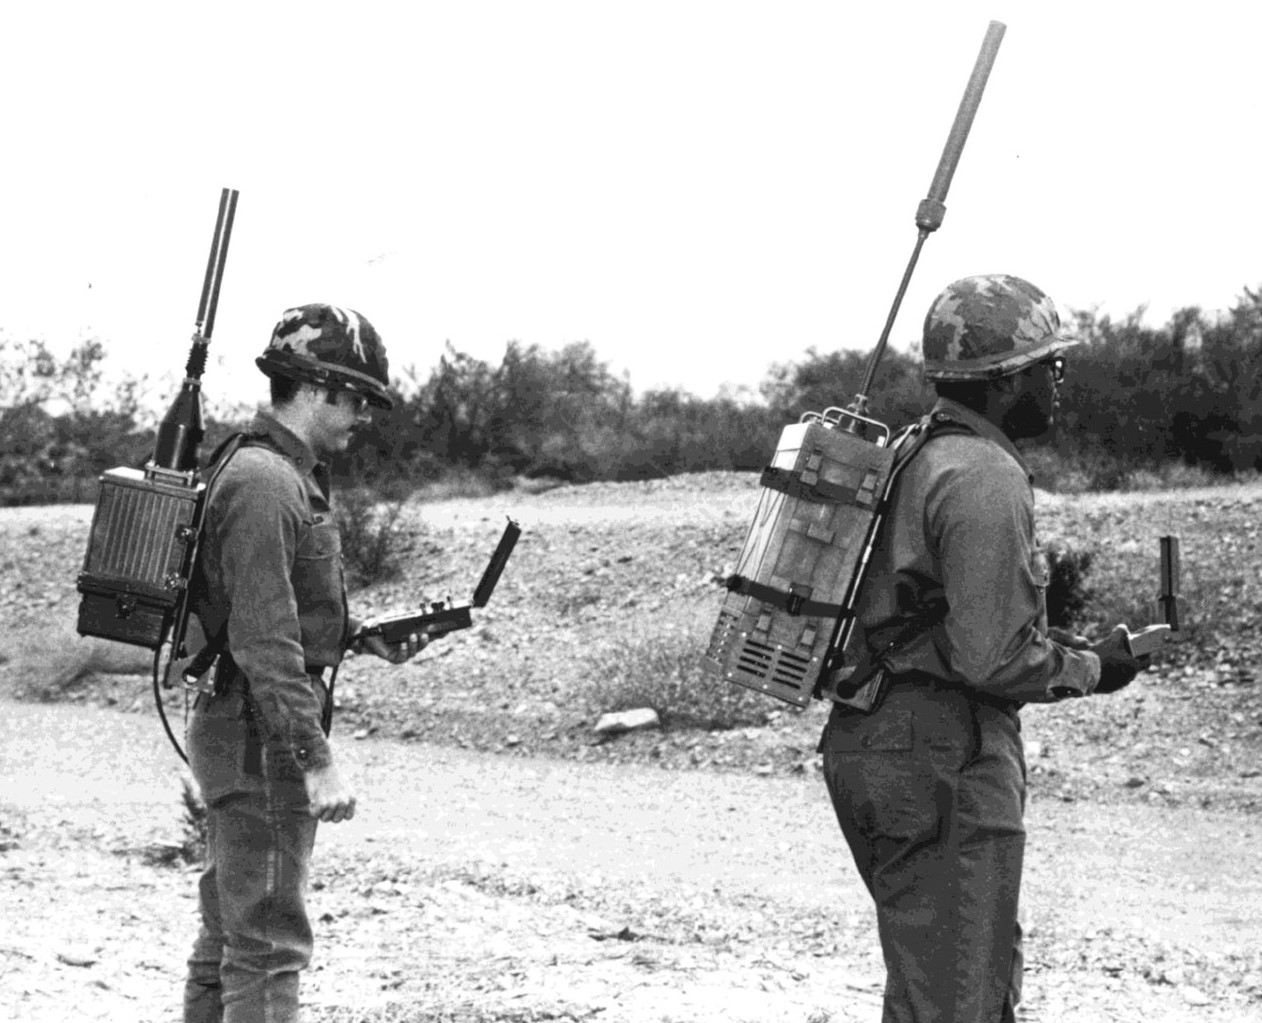
\includegraphics[width = 0.65\textwidth]{figures/historyGPS.jpg}
		\caption{Early GPS receivers were large, heavy devices. \cite{USAF1978}}
		\label{fig:2:histGPS}
	\end{center}
\end{figure}
Global Positioning System (GPS) is an everyday thing in our lives today and has become a luxury that most take for granted. There is GPS in our phones, laptops and even cars. We are using it to find directions on our commutes, hail taxis or ride shares and even for recreational sport, tracking how far we travelled.\par
\vspace{0.6cm}
The origins of GPS or rather any global satellite navigation system begins with the space race. It starts, in 1957, with the first satellite to successfully orbit the earth, the Russian satellite Sputnik. During its orbiting flight of the earth, Sputnik was emitting a radio signal which could be picked up on earth. During this orbit scientists from John Hopkins University in America were monitoring the radio signals emitted by the Sputnik satellite when they saw the Doppler Effect in action with the radio signals, as the satellite drew closer, the radio signal frequency increased and vice versa. These scientists theorized that if they could determine the location of the satellite based on its signal frequency, the opposite would also be true, they could determine the location of a receiver on the ground given the satellites location. \cite{Aerospace2021}\par
\vspace{0.6cm}
The first instance of a global satellite navigation system was the Transit. It was developed in 1958 by the Advanced Research Projects Agency and the first satellite was launched in 1960. The Transit satellites were mostly used by the military, specifically the Navy's missile submarines. The program was transferred to the Navy during the mid-1960s. During this time there were further Transit satellites launched and by 1968 the entire constellation of Transit satellites was operational, a total of 36 satellites. \cite{Aerospace2021}\par
\vspace{0.6cm}
There was plenty of other research that was being conducted around the same time to improve on the current Transit. One such researcher was Phillip Diamond. Diamonds concept, from his study in 1963, lead to the Air Force forming a new satellite navigation program which he called 621-B. Further studies were undertaken by James Woodford and Hideyoshi Nakamura, which completed in 1966, proposed using four satellites. The use of four satellites would mean that the receivers no longer needed to be equipped with high-accuracy clocks. This was the first step in reducing the size and cost of the receivers. \cite{Aerospace2021} \par
\vspace{0.6cm}
There was a range of technological advancements that help progress the satellite navigation systems such as new bandwidth utilization techniques, advancements in computers and the introduction of solid-state microprocessors. These technological advancements helped reduce the size and weight of the GPS receivers to what we now know today. Figure \ref{fig:2:histGPS} shows how large and cumbersome the early GPS receivers were. However, one significant technological advancement was the development of atomic clocks. This development led to another satellite navigation system known as Timation (Time Navigation). The third of three Timation satellites launched in 1974, became the first satellite equipped with an atomic clock, the previous two contained crystal oscillator clocks. The use of the atomic clock led to vast improvements in the accuracy of the navigation system and provided three-dimensional location coverage. \cite{Aerospace2021} \par
\vspace{0.6cm}
There were now three satellite navigation systems, and so when in the 1970s, the Department of Defence wanted a robust and stable system, the project team developed a new concept by cherry-picking the best aspects of all three, Transit, Timation and 621-B. This system was designated, Navigation System with Timing and Ranging (NAVSTAR), this was later changed to GPS I, the precursors to the GPS system we know today. The first NAVSTAR satellite was launched in 1978 and further satellites were launched in the following years, the system reaching its fully operational state with 24 satellites in 1993. \cite{Mai2017}\par
\vspace{0.6cm} 
Although the satellite navigation systems were operational and orbiting the earth, they were still used mostly by the military and the receivers were expensive. However, this began to change in 1983 when President Ronald Reagan authorized commercial airlines use of the NAVSTAR system. This was the start of civilian use of GPS. \cite{HistGPSProgram}
\par
\vspace{0.6cm} 
\subsection{Modern GPS}
The cost of GPS receivers began to decrease in the late-1990s, early-200s, the first cell phone containing GPS technology was released in 1999. The cost reduction can be attributed to the American government approving more non-military signals as well as the technological advances in processors that was leading to cheaper processing chips. And naturally from the cheaper access, GPS use began to grow, putting more tax on the system which although upgraded to GPS II was not equipped to handle the modern requirements. In 2000 a plan was formed to add new signals to satellites that had not yet been launched in order to handle the increased use. Furthermore, a new system was to be developed, GPS III, that could fully meet the modern requirements. The first of the GPS III satellites was launched in 2018 with a couple more in the following years and the remaining 6 to be launched by 2023. \cite{Aerospace2021}
\subsection{How GPS works}
\begin{figure}
	\begin{center}
		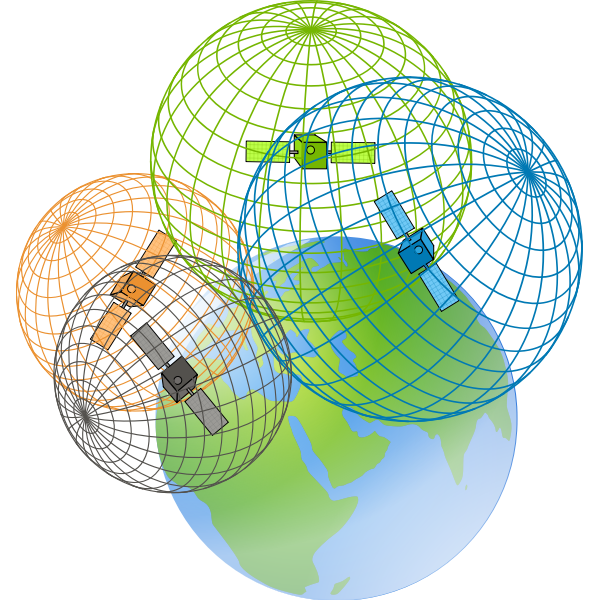
\includegraphics[width = 0.5\textwidth]{figures/GPStriangle.png}
		\caption{Distance spheres around each satellite intersect at one point}
		\label{fig:2:tiangleGPS}
	\end{center}
\end{figure}
There are a total of 31 GPS satellites currently sitting in a medium earth orbit. These are the satellites that are sending the radio signals that a GPS receiver can use to determine its location.\par
\vspace{0.6cm}
The signal that the satellites broadcast has a range of information that is used by receivers. This information contains data needed to determine the location of the satellite as well as the time that the signal broadcast, using the satellites atomic clock. Based on the time taken for the signal to reach the receiver and corrected for propagation delays or delays from the signal passing through the ionosphere and troposphere, the receiver can calculate the distance between itself and the satellite. This creates a sphere around the satellite upon which the receiver must lie. By adding in a second and third satellite and their distance spheres, there will be only two points of intersection between the three spheres. The one will be the receiver's location, while the other will be impossible location in space. However, to accurately calculate the distance, the receiver would have to have a synchronized atomic clock to determine exactly how long the signal takes to reach it. As it was mentioned earlier, highly accurate clocks were taken out of the receivers by adding a measurement from a fourth satellite to ensure that the distance calculation is accurate. Figure \ref{fig:2:tiangleGPS} illustrates the concept of the distance spheres and their intersection being the location of the GPS receiver. \cite{FederalAviationAdministration}
\section{Digital Compass}
Compasses have been used extensively over the past centuries for navigating, surveying, and map-making. The compass is thought to have been in use from around the 12th century in Europe and possibly earlier in east Asia \cite{Jones2019}. Although as many things have over the years been digitalized, so has the compass. The digital compass uses a technology called magneto-induction. This allows the digital compass to electronically detect the earth's magnetic field. Being as sensitive as it is, an embedded microcontroller is needed to filter out any magnetic fields from ferro-magnetic materials or other electrical systems that are creating a magnetic field. \cite{AdvancedSafetyDevices2013}
\subsection{What is magnetic north}
\begin{figure}
	\begin{center}
		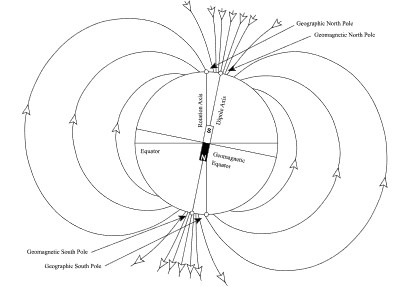
\includegraphics[width = 0.65\textwidth]{figures/tiltedDipole.jpg}
		\caption{The differentiation between magnetic and true north}
		\label{fig:2:magNorth}
	\end{center}
\end{figure}
True north is always fixed and is the direction that is directly in line with the north pole. However, compasses do not point to true north, they point to magnetic north. This is because a compass aligns itself with the magnetic field caused by the earth's magnetic core. The deviation between true north and the magnetic field at magnetic north is shown in figure \ref{fig:2:magNorth}. To further complicate the matter however, the earth's magnetic core experiences changes and these cause small shifts in the magnetic field around the earth which alters the deviation between true north and magnetic north. \cite{Jones2019}
\section{PWM}
\begin{figure}
	\begin{center}
		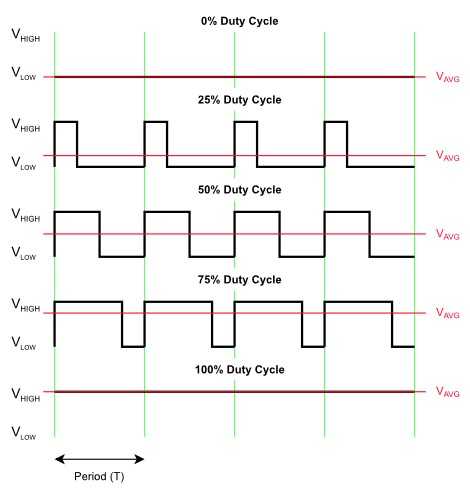
\includegraphics[width = 0.5\textwidth]{figures/PWM.jpg}
		\caption{Duty Cycle of PWM Signal}
		\label{fig:2:PWM}
	\end{center}
\end{figure}
Pulse Width Modulation (PWM) is a technique of using a digital signal to represent an analogue signal which is used to control analogue systems. The cost of switching a digital circuit between on (high) and off (low) is a cheaper alternative to creating an analogue circuit that will incur no drift over time. These PWM signals are mostly used in speed control of DC motors or controlling the brightness of light bulbs. \cite{Christ2014}\par
\vspace{0.6cm}
PWM is a digital signal that is switched between high and low, leading to the generation of a square wave signal. The time that the signal goes high can be modulated to vary the power delivered to the system. Typically, microcontrollers are used to generate and control the PWM to power an external system. There are a few signal parameters that will be highlighted in this explanation of a PWM signal. \par 
\vspace{0.6cm}
The signal amplitude: This is the maximum voltage that can be supplied to the external system. If the microcontrollers output voltage is insufficient for the external system, the signal can be passed through an amplifying circuit to provide the required voltage.\par 
The signal period: And therefore the frequency as they are inversely proportional, is the total time for one signal wave to propagate. The frequency is set depending on the requirements of the system, but this frequency will be needed later to help with the calculation of the duty cycle. \par 
The duty cycle: The ratio between the time the signal is high and the time the signal is low. It is always a value between 0 and 1, however, the duty cycle is often expressed as a percentage.\par
\vspace{0.6cm}
A PWM varies the voltage supplied to the system by varying the duty cycle. A small duty cycle means that the signal is high for a short portion of the signal period while a large duty cycle means that the signal is low for a large portion of the signal period. The system that is being supplied with power then uses the average voltage of this period. Therefore, a low duty cycle, a short high signal followed by a long low signal, would lead to a low average voltage. The variation in duty cycle and the associated average voltage is shown in figure \ref{fig:2:PWM}. \cite{Ibrahim2014}\par
\vspace{0.6cm}
To determine how long the signal must go high, the duty cycle is multiplied by the signal period. The duty cycle is often expressed as a percentage and so the duty cycle is the percentage of time that the signal is high. Therefore, by multiplying the duty cycle with the period gives the time for which the signal is pushed high (t1). Figure \ref{fig:2:PWMPulse} shows the relationship between t1, the time the signal is high, and T, the signal period.\par
\vspace{0.6cm}
\begin{figure}
	\begin{center}
		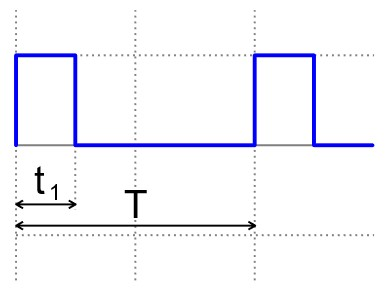
\includegraphics[width = 0.65\textwidth]{figures/PulseWideWave.jpg}
		\caption{The relation between the time the signal is high and the signal period.}
		\label{fig:2:PWMPulse}
	\end{center}
\end{figure}
\section{Analogue vs Digital Signals}
\begin{figure}
	\begin{center}
		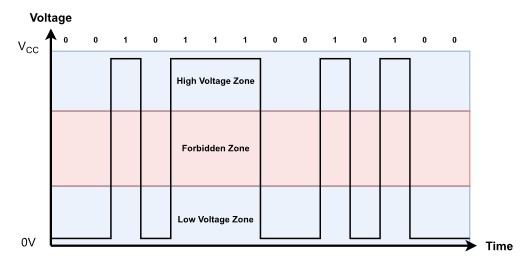
\includegraphics[width = 0.75\textwidth]{figures/DigitalSignal.jpg}
		\caption{A digital signal and its three zones.}
		\label{fig:2:digital}
	\end{center}
\end{figure}
Signals are used to convey data and information from point to point. For this project only electrical signals will be used although there are plenty of other mediums through which signals can be sent. There are two predominant signals that are used when regarding electrical signals, analogue and digital. \par
\vspace{0.6cm}
A digital signal, most simply represents discrete values, more precisely 2 discrete values. This makes digital signals perfect for conveying data in a binary data format but slightly more troublesome when more than two values are required. It will transmit a signal as either a low voltage, a zero, or a high voltage, a one. The low voltage is generally 0V while the high voltage is the voltage supply of the driving device. However, because voltages can have small fluctuations and will therefore not always be exactly 0V or equal to the nominal voltage, a range is pre-set whereby the receiving device can denote the value as low or high. A buffer zone is also incorporated, a voltage range around half the value of the nominal voltage, to prevent a small fluctuation in the voltage possibly altering the value of the signal. This buffer zone along with the area in which the signal can be read as high or low is shown in figure \ref{fig:2:digital}. This buffer is called the forbidden zone and any signal received within the forbidden zone is considered floating and will be randomly assigned as either high or low.\par
\vspace{0.6cm}
An analogue signal on the other hand is continuous and where the digital signal ranged from 0 to an upper voltage, an analogue signal ranges from a low voltage to a high voltage. Typically, $±V_CC$, the voltage of the microcontroller, is used for these upper and lower limits. An example of a continuous analogue signal between $±V_CC$ is shown in figure \ref{fig:2:analogue}. An analogue signal can therefore transmit an infinite number of values between these limits. By assigning an upper and lower limit to the sensor that will transmit the data, a max min transformation can be computed, and the transformed value transmitted along the analogue signal. Because the analogue signal is continuous, it can also be used in tracking the change in a value over time by computing the integral of the signal wave.\par
\begin{figure}
	\begin{center}
		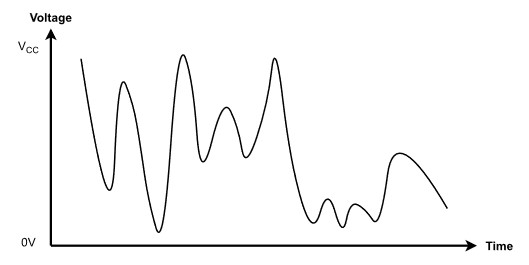
\includegraphics[width=0.75\textwidth]{figures/AnalogSignal.jpg}
		\caption{Analogue signal}
		\label{fig:2:analogue}
	\end{center}
\end{figure}



\chapter{Methodology and Design}
This chapter will describe the methodology used in the project. Firstly, it gives a general description of the system and how the components relate to each other and where they are on the system. This broad overview is to create a point of reference so that in later sections the specific details of the system can be discussed without spending too much time on the broader aspects. A brief discussion on the software enviroment is also included to provided a justification for the use of the chosen enviroment. Finally, the chapter will go into the design of the system. The design will discuss the objectives and requirements and then move onto the specifics of the hardware, electronics, software and the control system. The focus of this project is the control system and so the hardware discussion will focus on how it is relevant and how it is integrated with the system. The electronics form integral parts to the control system and so they are discussed in further detail and finally the software and control system are the focus of the project and will be described in full.\par
\begin{figure}[hb]
	\begin{center}
		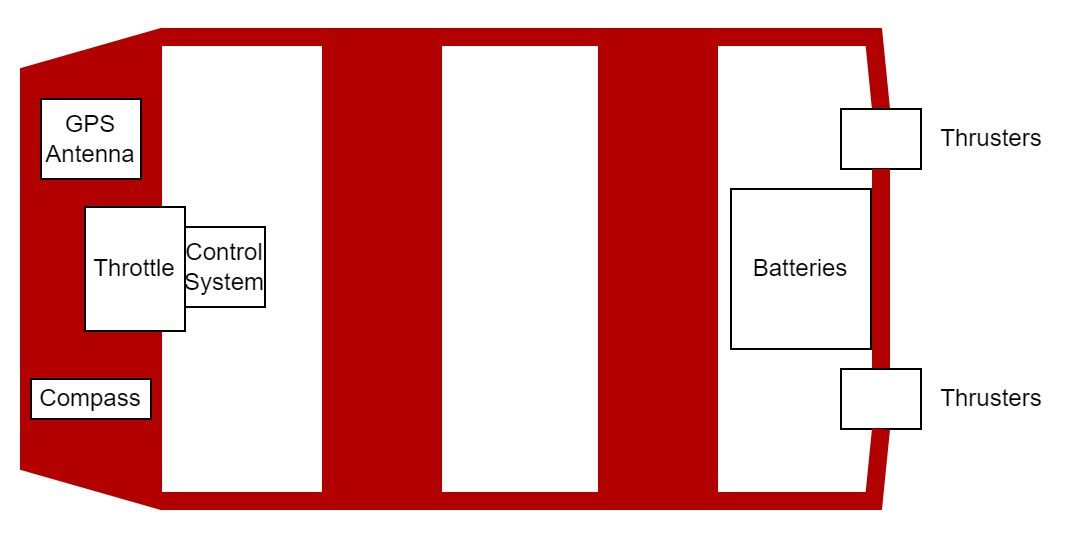
\includegraphics[width = 0.7\linewidth]{figures/BoatLayout.jpg}
		\caption{Broader System Diagram}
		\label{fig:3:boatDiag}
	\end{center}
\end{figure}
\section{System Description}
This section will give a broad overview of the system as a whole and  provide a reference of how the individual elements fit together both in the broader system and the narrower control system. The broader system is shown in Figure \ref{fig:3:boatDiag} and shows the vessel and the positions of the thrusters, batteries, control system throttle and mounting of the GPS antenna and compass. The control system refers to the 'motherboard', a PCB containing the microcontroller and other electronics including the GPS, SD module, logic level converter and the control box of switches and display LEDs. The wiring diagram of Figure \ref{fig:3:wiring} shows the PCB as a grey dotted line. The control box is shown outside of the PCB as it has its own housing but is affixed to the control system housing and is therefore considered part of the control system. Figure \ref{fig:3:wiring} also shows the wiring to the other elements that can be seen on the broader system diagram of Figure \ref{fig:3:boatDiag}. \par
\begin{figure}[ht]
	\begin{center}
		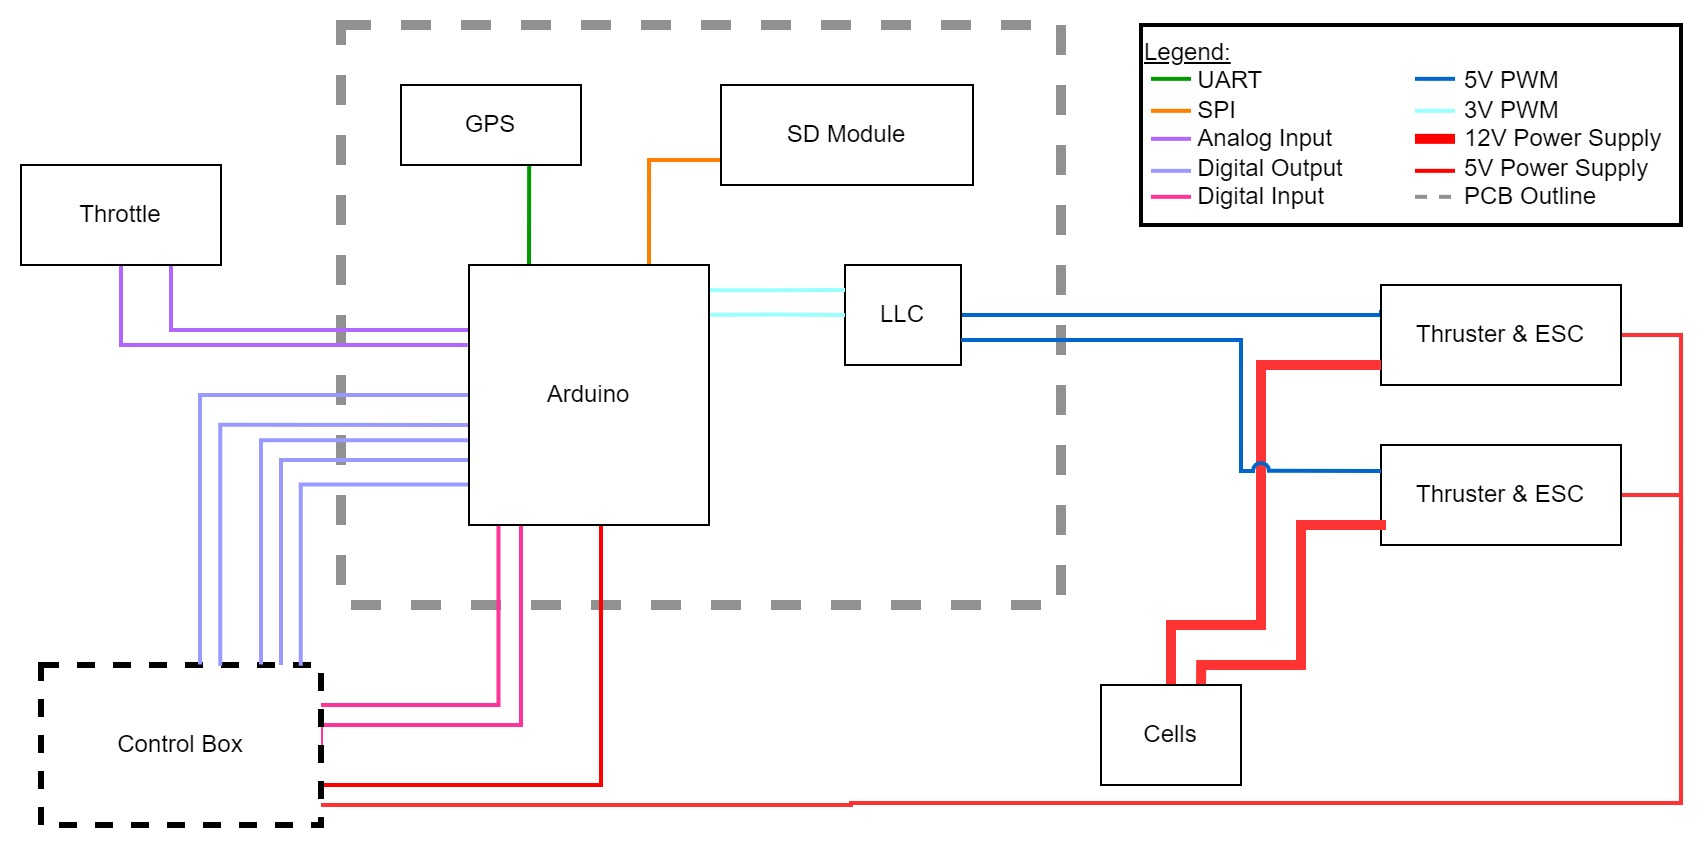
\includegraphics[width =\linewidth]{figures/Wiring diagram.jpg}
		\caption{Wiring Diagram for the System}
		\label{fig:3:wiring}
	\end{center}
\end{figure}

\section{Software Environment}
The microcontroller that was chosen for this project is an Arduino DUE. An Arduino microcontroller was chosen for the wide range of Arduino libraries available online, as well as several forums and code examples. Furthermore, the Arduino environment uses the C language which has been extensively covered through the course of the engineering degree. \par
\section{System Design}
	\subsection{Objective}
	The system needs to be designed to be deployed for long periods of time between services. The future addition of power regeneration such as solar or wind can be used to improve the deployable range and period of the vessel, but the energy storage must be designed to handle an extended period of 'dark time', any time when the power regeneration is negligible. \par
	The vessel must be autonomous and, having received a set of navigation points before deployment, navigate between these points until retrieval. Even under non ideal circumstances the vessel should be able to correct its course and continue to navigate to the set navigation points. \par
	This system is a proof of concept that is designed to be able to be sized up to a larger vessel. Therefore, the prototype vessel should be able to handle any conditions that could be encountered in testing and all electronics should be sufficiently sealed so that no damage is incurred. It is not expected that the prototype vessel would be able to handle rough and storm weather conditions.\par
	\subsection{Engineering Requirements}
	The prototype is a proof of concept that can be scaled up to a larger vessel and so a small vessel that can accommodate at least two people is required. This is preferred to a smaller vessel which cannot accommodate the weight of a person as the weight to power ratio of a small vessel could have an adverse effect on the steering capability of the vessel and therefore the control system.
	Furthermore, a working vessel is going to require a large battery bank and this is easily accommodated in a larger vessel. The energy source can then be scaled up by adding cells in both parallel and series to create the required power supply for the working vessel.\par
	The autonomous nature of the vessel means that an electronic control system is required to control the vessel. There are other elements that are required to make up the system, however these are not integral to the autonomous nature of the system but integral to the entire system. \par
	\subsection{Differential Steering} 
	Most ships and sea going vessels use a rudder or a directional thrusters to manoeuvre and this often simpler as it can be done with one thruster. However, in this project, the system has two thrusters and will make use of differential steering. Differential steering uses the two thrusters working at different thruster levels to steer the vessel. The outside thruster is at full power and the inside thruster is powered down and can even be put into reverse to manoeuvre the vessel. The most popular use of differential steering is in tracked vehicles such as military tanks. This project will use a system of progressive steering. Depending on how much the system needs to steer will determine how much thrust is given by the inside thruster. For example: for full steering the inside thruster will have \SI{100}{\percent} reverse thrust but for only a small steering correction the inside thruster could be powered down to \SI{80}{\percent}.
\begin{figure}
	\begin{center}
		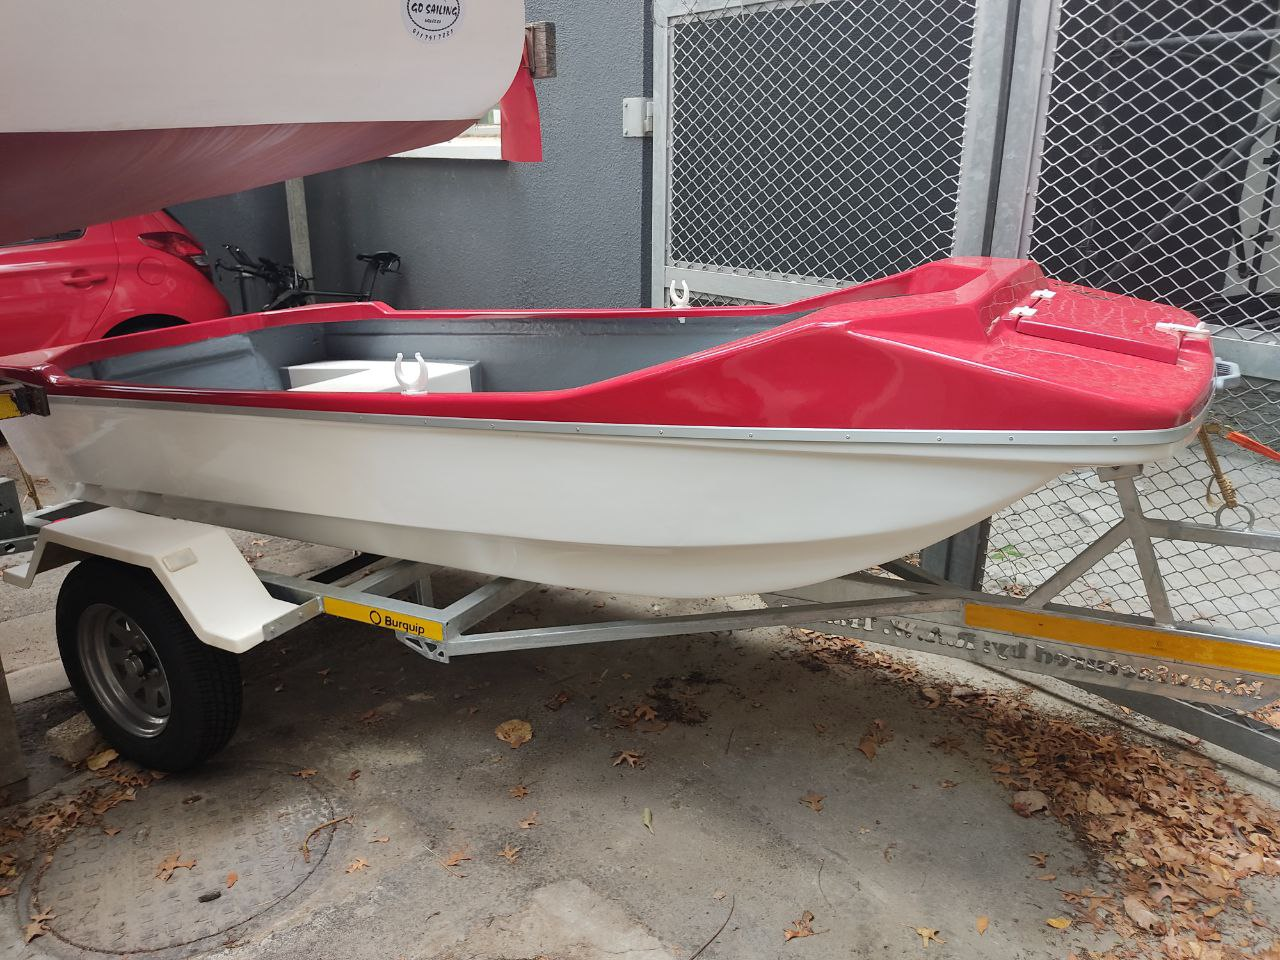
\includegraphics[width = 0.65\textwidth]{figures/spider3.jpg}
		\caption{The vessel, a Spider 3.}
		\label{fig:3:spider}
	\end{center}
\end{figure}
	\subsection{Hardware}\par
		\subsubsection{Vessel}
		The vessel is outside the scope of this project as it was acquired before the start of the project. The project was designed around the use of the vessel for testing only as in actual use a vessel would be used that could handle severe weather conditions and hold an array of sensory equipment. The vessel pictured in Figure \ref{fig:3:spider} is a Spider 3, a small single hulled fibreglass boat. The vessel measures \SI{1.3}{\meter} $\times$ \SI{3.2}{\meter} and is rated to carry four people and a 15 Hp traditional outboard motor.\par
		\subsubsection{Thrusters}
		The thrusters are electrical and a complete unit together with the ESC, and all the electronic interfacing to drive the thrusters is accomplished through it. The ESC is described later in the report. Therefore, the thrusters are considered general hardware and are there only as a means of testing the control system. They are outside the scope of the project as they were acquired prior to the start of the project, but are integral to the performance of the overall system.\par 
		The propulsion system consists of two electric thrusters mounted at the back of the vessel. These thrusters are each capable of producing up to \SI{18}{\kilogram} of thrust. An aluminium mount designed and manufactured by the Stellenbosch University Electrical Engineering workshop allows for the thrusters to be raised during the launching and retrieval of the boat to avoid fouling on the trailer. The mounts are removable and are removed for transport. Each thruster has an integrated ESC that regulates the power supplied to the electric motor and therefore the thrust provided.
		\subsubsection{Power Supply}
		The initial design was to use a bank of four Lithium Iron Phosphate (LiFePO) cells to form a \SI{12}{\volt} battery. This was also procured before the start of the project. However, upon testing, it was seen that \SI{12}{\volt} was not enough voltage to provide the thrusters with enough power to move the boat at a reasonable rate. Each cell has a voltage of \SI{3.3}{\volt} and a capacity of \SI{100}{\ampere\hour}. Therefore, the next course of action was to source more cells and increase the size of the battery. However, due to the high cost of these cells and a lack of suppliers this was not plausible. LiFePO cells are expensive because they are designed to have a deeper life cycle than standard lead acid cells. These cells in particular were also expensive due to their large capacity.\par 
		Therefore, the decision was made to change the power source to a battery consisting of two lead acid cells in order to test the control system. The lead acid cells were each \SI{12}{\volt} and had a capacity of \SI{50}{\ampere\hour}. A lead acid battery can generally be drained to about \SI{80}{\percent} capacity without doing much damage to the cell, a LiFePO cell has a deep cycle of about \SI{40}{\percent}-\SI{50}{\percent}. Therefore these cells would be used for short tests and recharged between tests. However, for a working system it would be recommended that a large LiFePO battery bank were used. 
		\begin{figure}[!ht]
			\begin{center}
				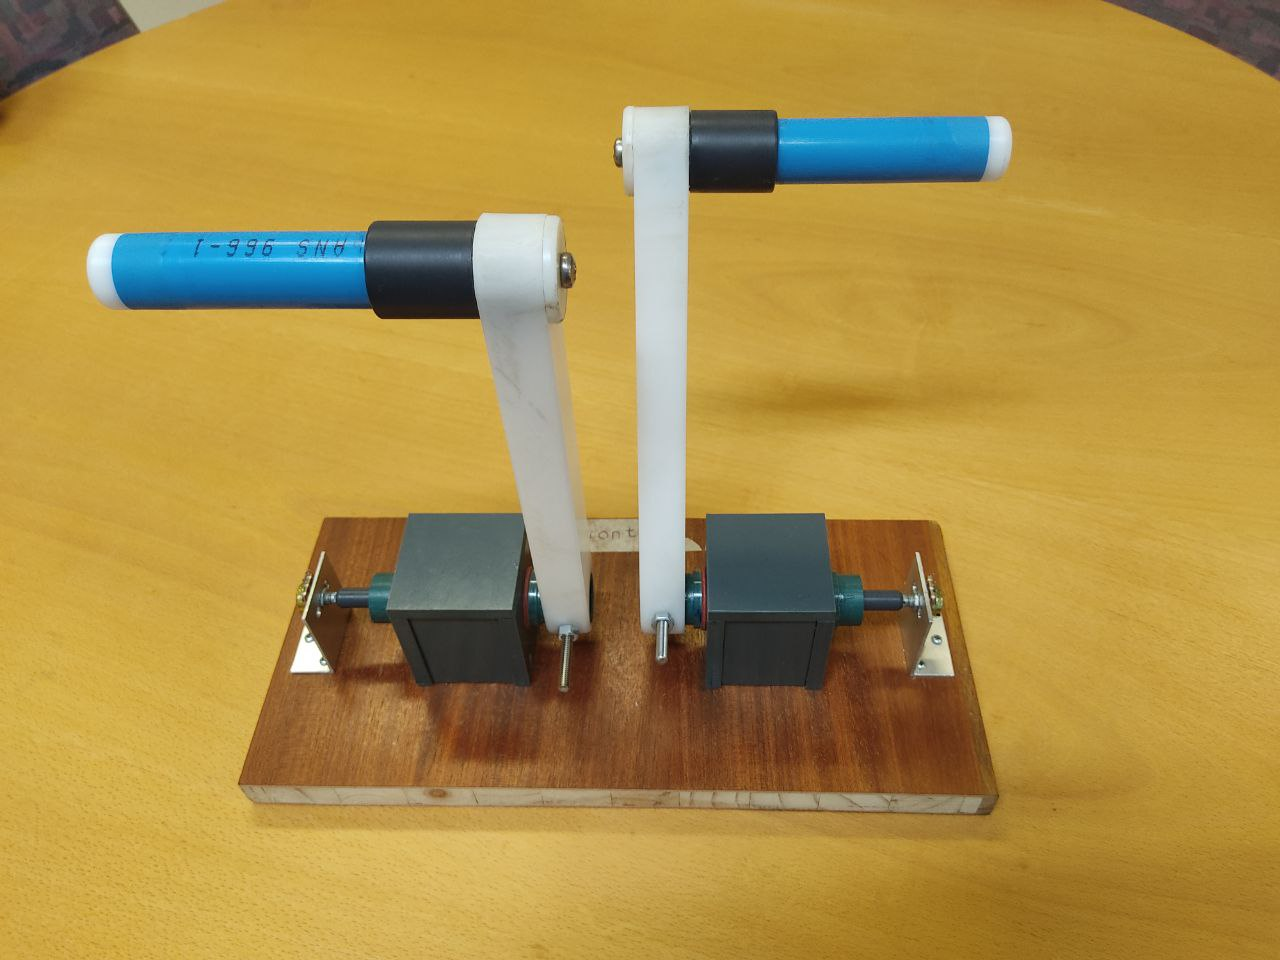
\includegraphics[width = 0.55\textwidth]{figures/throttle.jpg}
				\caption{Final throttle system with two potentiometers (POT) on either end.}
				\label{fig:3:throttle}
			\end{center}
		\end{figure}
		\subsubsection{Throttle}
		The initial concept was to purchase two throttles capable of moving independently from each other and two electronic throttle levers were purchased to be used. However, when these components arrived, they were much smaller than they had appeared and had a very small range of movement. An alternate solution was designed consisting of two throttle arms that could each turn a shaft. These shafts were then connected to a linear potentiometer which would provide the required analogue input from the throttle. The throttle is shown in Figure \ref{fig:3:throttle}. An initial concept design was given to the electrical engineering department who then refined and manufactured the design. 
		\par
	\subsection{Electronics}\par
		
		\subsubsection{Arduino Due}\par
		\begin{figure}[!ht]
			\begin{center}
				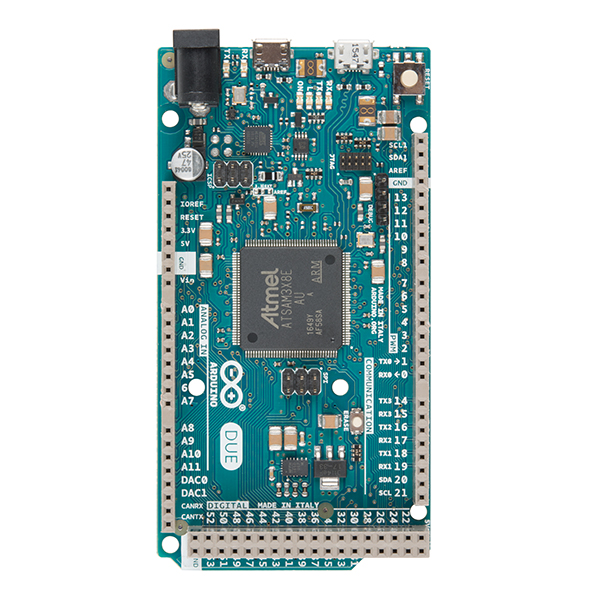
\includegraphics[width = 0.48\textwidth]{figures/DUE.jpg}
				\caption{The microcontroller used: an Arduino DUE}
				\label{fig:3:due}
			\end{center}
		\end{figure}
		The microcontroller was selected by considering the initial design and possible peripherals that would be used in the system. The minimum requirements for the microcontroller to be used are as follows, with regard to the peripherals of the GPS, SD card modules, the ESC and POTs as well as several inputs and outputs:
		\begin{enumerate}
			\item 2 PWM pins.
			\item Voltage regulators of \SI{3}{\volt} and \SI{5}{\volt}.
			\item 5 digital IO pins.
			\item 4 analogue input pins.
			\item 1 SPI connection.
			\item 1 UART connection.
			\item 1 I\textsuperscript{2}C connection.
			\item \SI{256}{\kilo\byte} programmable flash memory.		
		\end{enumerate}
		Based on these requirements, the Arduino Uno was considered. It is the standard Arduino board used in projects and meets most of the minimum requirements for the project.  However, the Arduino Uno has only one UART connection and does not allow for any possible design alterations that might need a second UART connection. Finally, the Arduino only has \SI{32}{\kilo\byte} of programmable flash memory which does not meet the requirements.\par 
		The next consideration was the Arduino DUE, shown in Figure \ref{fig:3:due} This has 4 UART connections, plenty of digital IO pins and several analogue inputs. This offers a range of versatility to any design progression or alterations that might occur. Furthermore, the DUE has \SI{512}{\kilo\byte} of programmable flash memory which is double that of the minimum requirement. The one flaw with the Arduino DUE is that its IO pins operate at \SI{3.3}{\volt} as opposed to the generally standard \SI{5}{\volt}. However, this was easily overcome by implementing a logic level converter to shift the required signals to \SI{5}{\volt} while keeping the signals' shape. Keeping the signals' shape is particularly important for the PWM signal controlling the ESCs. The final microcontroller selected was the Arduino DUE. \cite{Corporation2015}
		\subsubsection{SD Card Module}
		The SD card is used as an external storage device. Data can then be written to the SD card during operation and the data can be downloaded for analysis. The SD card module is a standard SD card module that is attached to the microcontroller as shown in the wiring diagram Figure \ref{fig:3:wiring}. The SD card uses SPI communication and there are built-in libraries that are available for use. \cite{Association2017}
		\subsubsection{GPS Module}
		Initially a PmodGPS was used as the GPS module. However the PmodGPS has a built-in antenna and there were signal strength issues. The GPS was slow at acquiring a GPS fix when the control box was closed. Therefore, an alternate GPS module with an external antenna was sourced. The antenna can be fed out of the control box and positioned where a strong signal can be received. Both GPS modules use UART to communicate the data to the microcontroller. The GPS modules send a string of characters along the UART connection, and the microcontroller must then decode the characters. The GPS module transmits the current longitude, latitude, date and time and speed of the vessel to the microcontroller. The UART is set-up to use a baud rate of 9600, 8 data bits, no parity and 1 stop bit. It has two connectors J1, which has 6 pins and J2 which has 2 pins. J1 is used to power the GPS module as well as connect to the MCU using UART communication. \cite{Robot}
		\subsubsection{Compass}
		The digital compass used can be more accurately referred to as a magnetometer. The module used in this project, a  Pololu LSM303 shown in Figure \ref{fig:3:compass}, is a combination magnetometer and accelerometer, however only the magnetometer is used. Pololu has a range of Arduino libraries including a compass library for the LSM303 which is used to calibrate the module and to get an accurate compass bearing. \cite{STMicroelectronics2015}
		\begin{figure}[!hb]
			\begin{center}
				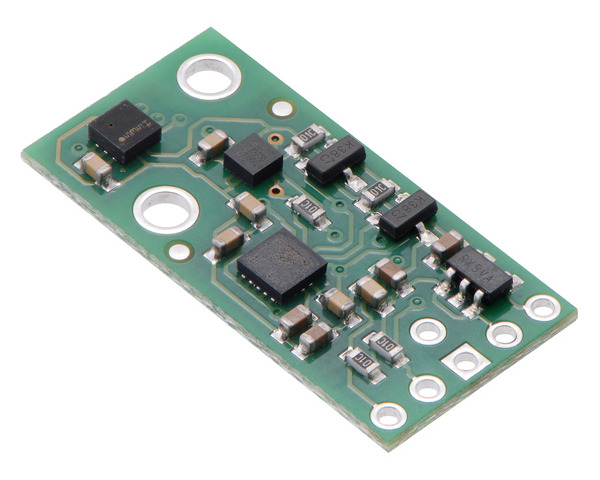
\includegraphics[width = 0.16\textwidth]{figures/compass.jpg}
				\caption{Pololu LSM303 AltIMU module.}
				\label{fig:3:compass}
			\end{center}
		\end{figure}
		\subsubsection{ESC}
		There are two ESCs, one for each thruster and are submersible. The ESC has two inputs, the control input, and the power input. Th power input can range between DC \SI{12}{\volt} and DC \SI{50}{\volt} and a maximum constant current of \SI{100}{\ampere} and in this project the input is \SI{24}{\volt} supplied by the battery cells. The control input is a \SI{5}{\volt} signal that is used to control the speed of the thrusters. This is a PWM signal whose duty cycle determines the thrusters RPM and therefore the speed and direction of the vessel. 
		\subsubsection{POT}
			\begin{table}[ht]
			\begin{center}
				\caption{The digital values of the ADC used to calibrate the physical limits and neutral range of the throttle potentiometers.}
				\label{tab:3:POT}
				\begin{tabular}{|l|c|c|}
					\hline		
					\textbf{Throttle Position} & \textbf{Left POT} & \textbf{Right POT} \\
					\hline
					Full Forward & 655 & 720\\
					\hline
					\multirow{2}{*}{Neutral} &440 &505 \\
					&485 &572  \\
					\hline
					Full Reverse & 285 & 352 \\
					\hline
				\end{tabular}
			\end{center}
		\end{table}
		The POT is a standard \SI{10}{\kilo\ohm} potentiometer that has three pins as shown in Figure \ref{fig:3:POTdraw}: high voltage, ground, and output. The high voltage and ground are connected to the outer pins on the POT and the output is connected to the centre pin. As the shaft of the potentiometer is rotated, the resistance varies from almost no resistance to the full \SI{10}{\kilo\ohm} which causes the voltage to vary from input, \SI{3.3}{\volt} to an almost ground voltage, ~\SI{0.1}{\volt}.  \par
		\vspace{0.4cm}
		\begin{figure}[hb]
			\begin{center}
				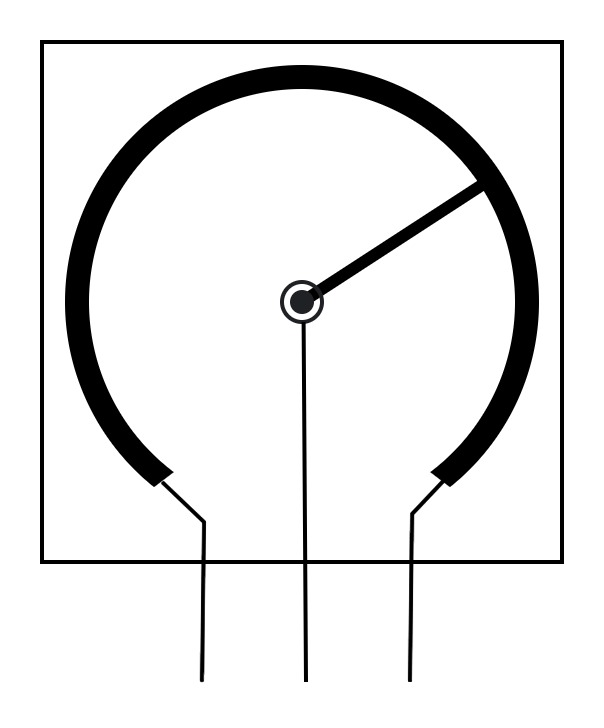
\includegraphics[width = 0.25\textwidth]{figures/POT.jpg}
				\caption{Simple illustration of a linear potentiometer}
				\label{fig:3:POTdraw}
			\end{center}
		\end{figure}
		The output is connected to analogue input pins on the microcontroller which uses an ADC, with a 10 bit resolution, to convert the signal to a value between 0 and 1024. However, the potentiometer has a \SI{300}{\degree} range of motion but the throttle has approximately \SI{150}{\degree} range of motion. The software can  correct for the difference by determining the total maximum and minimum range of motion of both throttle levers while in operation. The forward range is set between an offset middle point and maximum range for each device. Similarly, the reverse range is set between the offset middle point and the minimum range for each device.  This offers a neutral range buffer to make the throttle easier to use i.e. the controller can be placed in the neutral position by returning the lever to the general neutral position. The extents of the measured forward and reverse ranges are listed in Table \ref{tab:3:POT}.
	\subsubsection{Switches and LEDs}
	\begin{figure}
		\begin{center}
			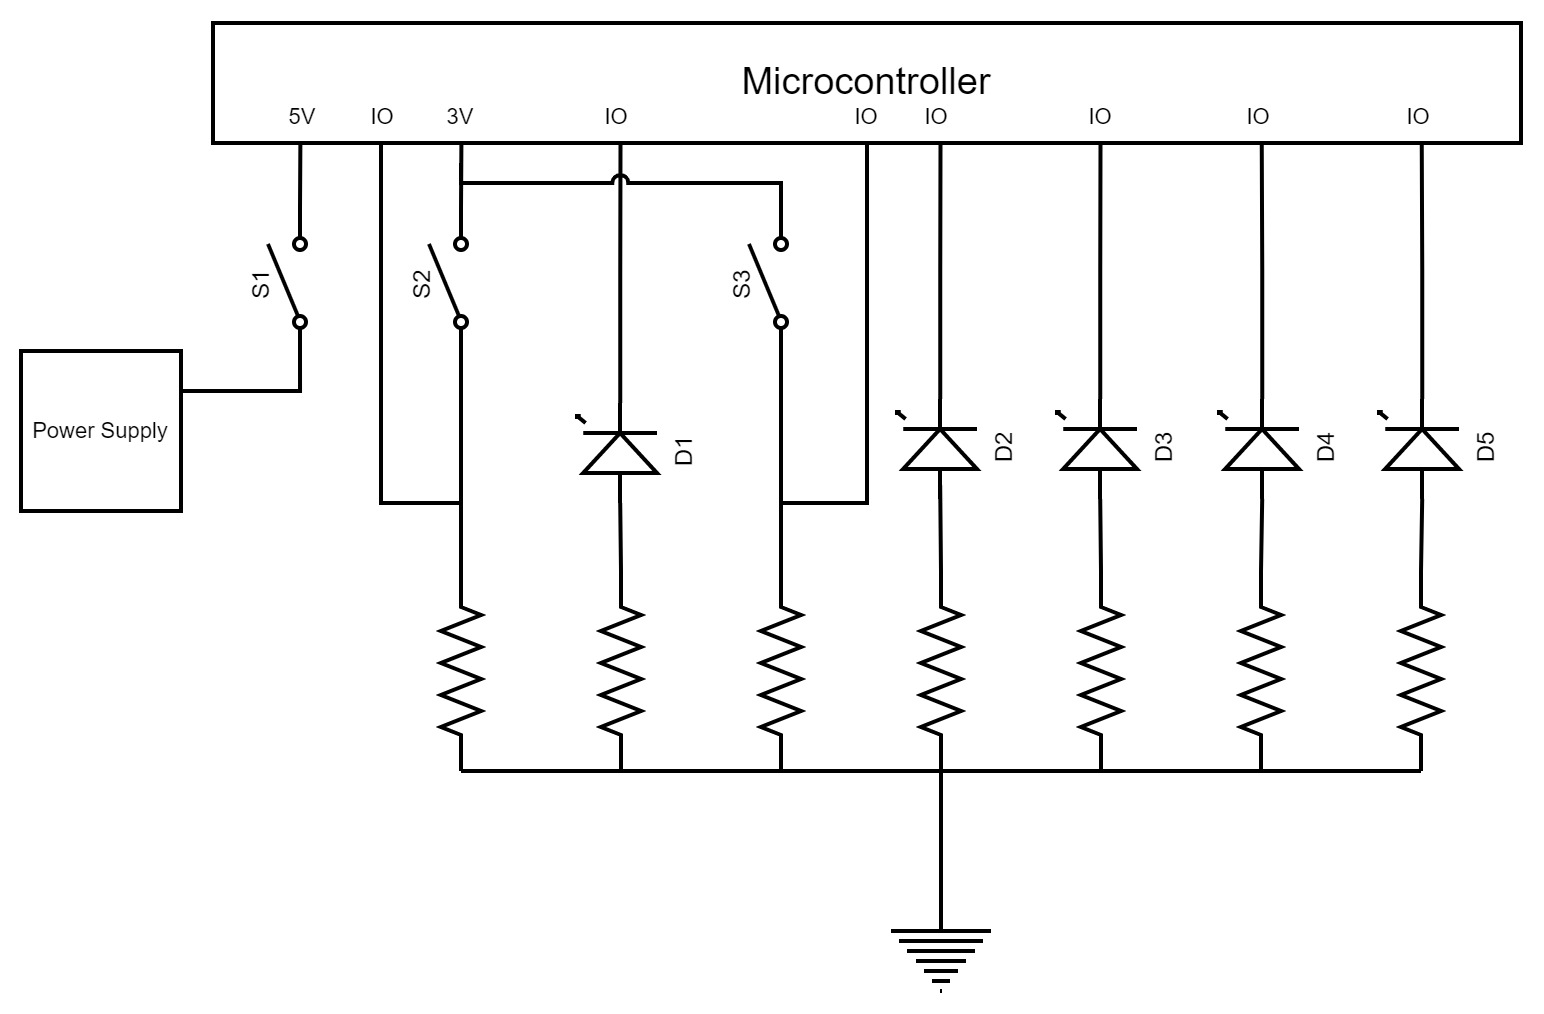
\includegraphics[width=0.65\linewidth]{figures/BoxCircuit}
			\caption{The wiring circuit inside of the control box.}
			\label{fig:3:controlCircuit}
		\end{center}
	\end{figure}
	The control box shown in Figure \ref{fig:3:controlBox} consists of 3 switches and 5 state display LEDs. Two of the switches are configured using pull down resistor configuration with the output of the pull down circuit connected to a digital input on the microcontroller. The LEDs all use simple LED circuits driven by the digital outputs of the microcontroller. The final switch, the power switch, is wired to cut-off the \SI{5}{\volt} power supply to the microcontroller. The control box circuit is shown in Figure \ref{fig:3:controlCircuit} and can also been seen in the overall wiring diagram of the system in Figure \ref{fig:3:wiring}. A description of each switch and LED is given in Table \ref{tab:3:controlBx}.
	\begin{figure}[hb]
		\begin{center}
			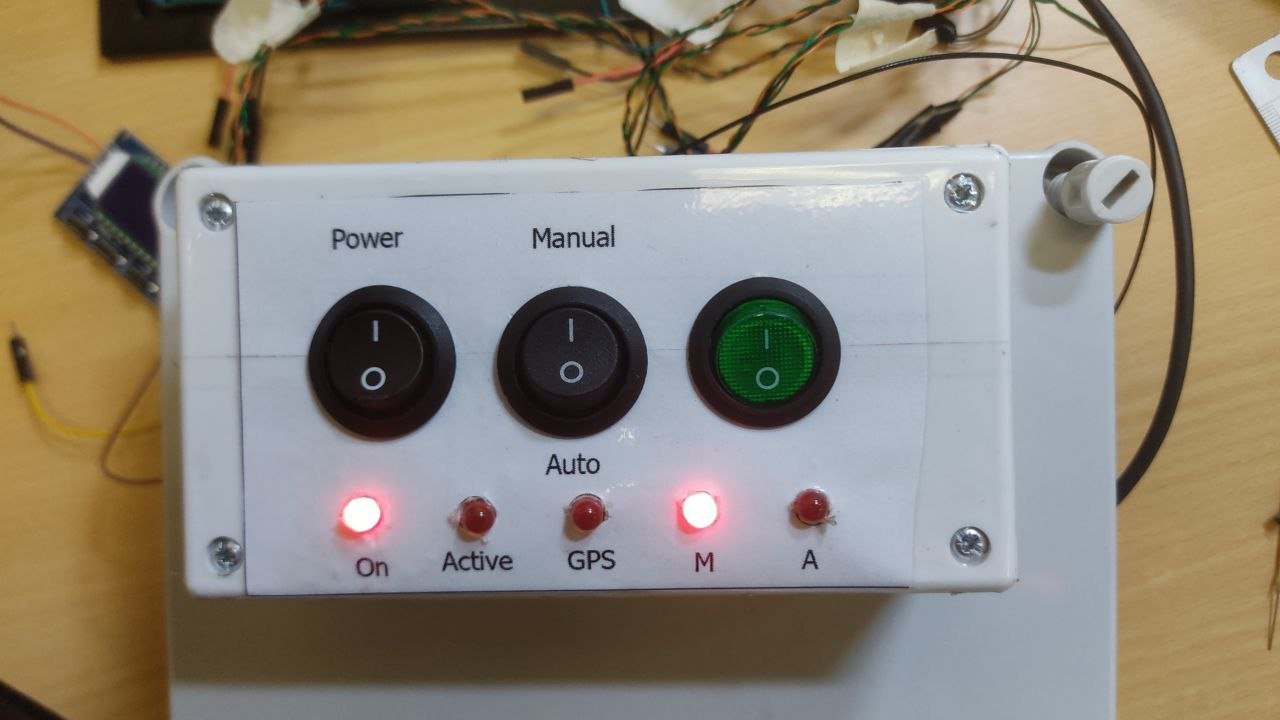
\includegraphics[width = 0.85\textwidth]{figures/controlBox.jpg}
			\caption{The control box with its 3 switches and 4 LEDs.}
			\label{fig:3:controlBox}
		\end{center}
	\end{figure}
	\begin{table}[ht]
	\begin{center}
		\caption{Description of the switches and LEDs on the control box.}
		\label{tab:3:controlBx}
		\begin{tabular}{|p{0.2\linewidth} | p{0.15\linewidth}|p{0.65\linewidth}|}
			\hline
			Component & Designation & Description \\
			\hline
			Power Switch & S1 & This switch is used to cutoff the power being supplied to the microcontroller. \\
			\hline
			Navigation Mode Switch & S2 & This switch allows the user to quickly switch between the manual navigation mode and the autonomous navigation mode. \\
			\hline
			Calibration Switch & S3 & This switch is used to put the system into compass calibration mode. \\
			\hline
			On LED & D1 & This LED indicates that the microcontroller is powered on. \\
			\hline
			Active LED & D2 & This LED blinks on and off during the operation of the program and indicates that the program is alive and active and there has not been a crash in the program. \\
			\hline
			GPS LED & D3 & This LED is turned on when GPS has a valid connection. \\
			\hline 
			M LED & D4 & This LED indicates that the system is in manual control mode. \\
			\hline
			A LED & D5 &  This LED indicates that the system is in autonomous navigation mode. \\
			\hline
		\end{tabular}
	\end{center}
\end{table}
	\subsection{Software}
	\subsubsection{PWM Signal}
	\begin{figure}[!hb]
		\begin{center}
			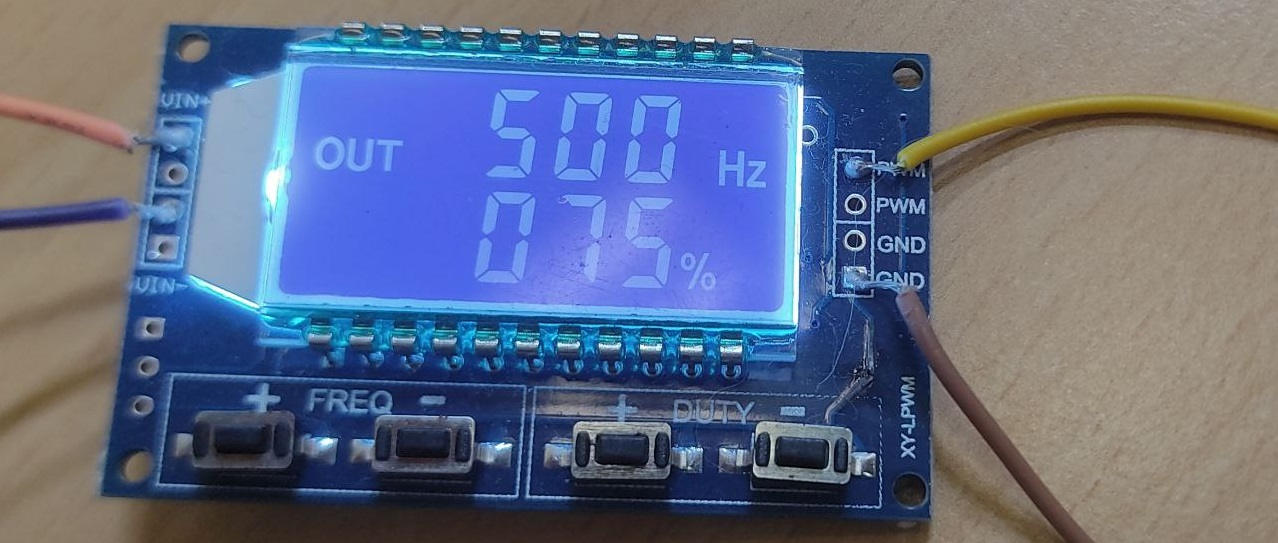
\includegraphics[width=0.31\linewidth]{figures/pwmGen.jpg}
			\caption{The PWM signal generator used to ensure the ESC was working.}
			\label{fig:3:PWMgen}
		\end{center}
	\end{figure}
	\begin{table}[!ht]
		\begin{center}
			\caption{ESC boundaries and PWM duty cycle at various frequencies.}
			\label{tab:3:PWM}
			\begin{tabular}{|l|c|c|c|c|}
				\hline
				\multirow{2}{*}{Position} & \multirow{2}{*}{Time (\SI{}{\micro\second})} & \multicolumn{3}{c|}{Duty Cycle @}\\
				%\hline 
				& & \multicolumn{1}{c}{\SI{50}{\hertz}} & \multicolumn{1}{c}{\SI{60}{\hertz}} & \multicolumn{1}{c|}{\SI{500}{\hertz}}\\
				\hline
				Full Forward & 2000 & \SI{10}{\percent} & \SI{12}{\percent} & \SI{100}{\percent}  \\
				\hline
				Neutral & 1500 & \SI{7.5}{\percent} & \SI{9}{\percent} & \SI{75}{\percent}  \\
				\hline
				Full Reverse & 1000 & \SI{5}{\percent} & \SI{6}{\percent} & \SI{50}{\percent}  \\
				\hline
			\end{tabular}
		\end{center}
	\end{table}
	The thrusters are each controlled by a \SI{5}{\volt} PWM signal. There is limited information on the datasheet for the ESC. The signal boundaries, full forward, full reverse and neutral positions are described in the unconventional terms of the time that the signal is high. The values are shown in Table \ref{tab:3:PWM}. Initially it was thought that the ESC operated at \SI{50}{\hertz}, however there was no response from the thruster at any duty cycle when using this frequency.A PWM signal generator IC, shown in Figure \ref{fig:3:PWMgen}, was connected to ESC to ensure  the correct PWM signal was being sent through and to quickly vary both the frequency and the duty cycle.  Trial and error later determined that the ESC began responding to a signal above \SI{60}{\hertz}. It was then decided to push the frequency up to the maximum of \SI{500}{\hertz} as this offers the finest control because it has the maximum allowable duty cycle difference between the signal boundaries.\par
	\vspace{0.4cm}
	The Arduino libraries contain a function, \textit{analogueWrite(value, pin)}, which takes the duty cycle and the output pin as parameters. This will output a PWM wave of the given duty cycle on the given pin. However, the default frequency of the Arduino DUE PWM pins is \SI{1000}{\hertz}. Therefore, the frequency had to be manually changed by changing the timer settings driving the PWM signal.\par
	\vspace{0.4cm}
	The information needed to change the timer settings is available in the Arduino Datasheet. The process to configure the PWM outputs is as follows. First, the peripheral clocks for timer channels 6 and 7 were enabled. Secondly, the pins' input-output controller on peripheral A needed to be disabled and the pins switched to peripheral B. Then came the configuration of the timer itself. The channel mode was set to waveform mode using clock 1 with the timer counter being incremented on the rising edge. Furthermore, the waveform was set to UP mode (signal is set high) being triggered when the counter reached the register C (RC) value and the signal being cleared when the counter reached the register A (RA) value. Once the timer is configured, values can be assigned to the RA and RC values, and the interrupt set to trigger when the counter reaches RC. Finally, an interrupt handler needs to be added to read the status register, since the flags in the status register are automatically reset when it is read at the end of every period.\par
	\vspace{0.4cm}
	The signal is cleared when the counter reaches RA and set high when the counter reaches RC. Therefore, RC can be equated to the period of the signal and RA to the time when the signal is high. Since the clock is set to clock 1 which is the MCU clock (MCK) divided by 2, and by using the above comparison, the RA and RC can then be expressed in terms of MCK, frequency and duty cycle, as shown in Equations \ref{eq:3:RC} and \ref{eq:3:RC}. RC is kept constant throughout while RA is changed to adjust the duty cycle of the PWM signal sent to the ESC, thereby controlling the ESC and thrusters.
	\begin{equation}
		RC = \frac{\frac{MCK}{2}}{Frequency}
		\label{eq:3:RC}
	\end{equation}
	\begin{equation}
		RA = RC \times Duty Cycle
		\label{eq:3:RA}
	\end{equation}
	\subsubsection{Analogue to Digital Converter}
	As mentioned previously, the ADC is used to convert the analogue signal from the potentiometers connected to throttle to a digital signal between 0 and 1024. Furthermore, using Table \ref{tab:3:PWM} and Table \ref{tab:3:POT} a relationship can be created to determine the RA value for a given throttle position. Because the forward operation is in the duty cycle range \SI{75}{\percent} to \SI{100}{\percent}, the analogue input from the POT needs to be linearly mapped to represent an equivalent duty cycle in this range. Equation \ref{eq:3:dutyF} shows how this is done for the forwards operation. The same logic can be used to determine the duty cycle for reverse as Equation \ref{eq:3:dutyR} shows. For neutral however, the RA value needs to be exact, but this is difficult to achieve using the throttle, therefore, a neutral range is used on the potentiometer whereby any value in the range will be seen as neutral and the neutral value will be written to the RA register. \cite{Corporation2015}
	\begin{equation}
		Duty Cycle_{Forward} = 100 - (100-75)(\frac{POT_{MAX} - POT_{Input}}{POT_{MAX} - POT_{Neutral}})
		\label{eq:3:dutyF}
	\end{equation}
	\begin{equation}
		Duty Cycle_{Reverse} = 75 - (75-50)(\frac{POT_{Neutral} - POT_{Input}}{POT_{Neutral} - POT_{MIN}})
		\label{eq:3:dutyR}
	\end{equation}
	\subsubsection{GPS}
	 The GPS module transmits a series of five sentences containing various information. Each sentence begins with a '\$GP' and then the specific message ID. The data is then sent through comma separated and finally ends with a checksum at the end of line characters <CR><LF>. For this project the Recommended Minimum Specific (RMC) sentence is the only sentence of interest as it contains all the necessary information: longitude, latitude and speed over ground in knots. An example of the RMC sentence is shown below.\par
	\vspace{0.2cm}
	\par
	\begin{center}
		\begin{tabular}{c}
			\small{\$GPRMC,064951.000,A,2307.1256,N,12016.4438,E,0.03,165.48,260406,3.05,W,A*55<CR><LF>}\\
		\end{tabular}
	\end{center}
	\vspace{0.4cm}
	The entire sentence is read by the MCU before it starts to pick the specific data out of the string using the commas and full stops as the guide to which array position is which data. The latitude and longitude are given in the format 'DDmm.mmmm' and must first be converted to decimal degrees as this is easiest to use in calculations. The Equation \ref{equ:3:degreeConv} shows this conversion. Each piece of data is then added to an instance of a GPS structure that can then be easily parsed to the navigation algorithm and analyzed. The variables within the GPS structure are shown in Table \ref{tab:3:GPSstruct}. \cite{Robot}
	\begin{equation}
		Decimal Degrees = Decimal + \frac{Minutes}{60}
		\label{equ:3:degreeConv}
	\end{equation}
	\begin{table}[!ht]
		\begin{center}
			\caption{Variables and their types within the GPS structure.}
			\label{tab:3:GPSstruct}
			\begin{tabular}{|l|l|l|}
				\hline
				\textbf{Name} & \textbf{Type} & \textbf{Description} \\
				\hline
				UTC & int & Coordinated Universal Time in the format (hhmmss). \\
				\hline
				latDecimal & int & The decimal portion of the latitude. \\
				\hline
				n\_s & char & A character indicating North or South. \\
				\hline 
				longiDecimal & int & The decimal portion of the longitude. \\
				\hline 
				e\_w & char & A character indication East or West. \\
				\hline
				knots & float & The speed over ground in knots. \\
				\hline
				course & float & The course over ground in degrees. \\
				\hline
				date & int & The date in the format (ddmmyy). \\
				\hline
			\end{tabular}
		\end{center}
	\end{table}
	\subsubsection{Compass}
	There was very little software to develop for the compass as there are extensive Arduino libraries which were used. The code used to calibrate the compass and to get the compass heading was all derived from the relevant calibrate and heading example projects provided by the libraries. \cite{Pololu2016}
	\subsection{Control System}
	The control system is the scope of this project and the part of the project that should not require much alteration to scale the system up to a larger system. The control logic  is all implemented through the software on the microcontroller. This section will detail the control logic with the aid of flow diagrams and pseudo code. 
		\subsubsection{State Machine}
		\begin{algorithm}[!hb]
			\caption{State Algorithm}
			\label{alg:3:mainWhile}
			\begin{algorithmic}[1]
				\Require{Declare variables and initialize PWM, SPI, I\textsuperscript{2}C and UART.}{}
				\BState \emph{loop}:
				\If{$\textit{manual control} = \textit{true}$}
				\State $\textit{call updatePWM()}$
				\State $\textit{call powerThruster()}$
				\Else 
				\State $\textit{call receivedGPSdata()}$
				\If{$\textit{GPS data is valid}$}
				\State $\textit{call navigate()}$
				\Else
				\State $\textit{Delay 1 second}$
				\EndIf
				\If{$\textit{Last point has been reached}$}
				\State $\textit{Halt receiving GPS data}$
				\EndIf
				\EndIf
				\State \textbf{goto} \emph{loop}.
			\end{algorithmic}
		\end{algorithm}
	\begin{figure}[!hb]
		\begin{center}
			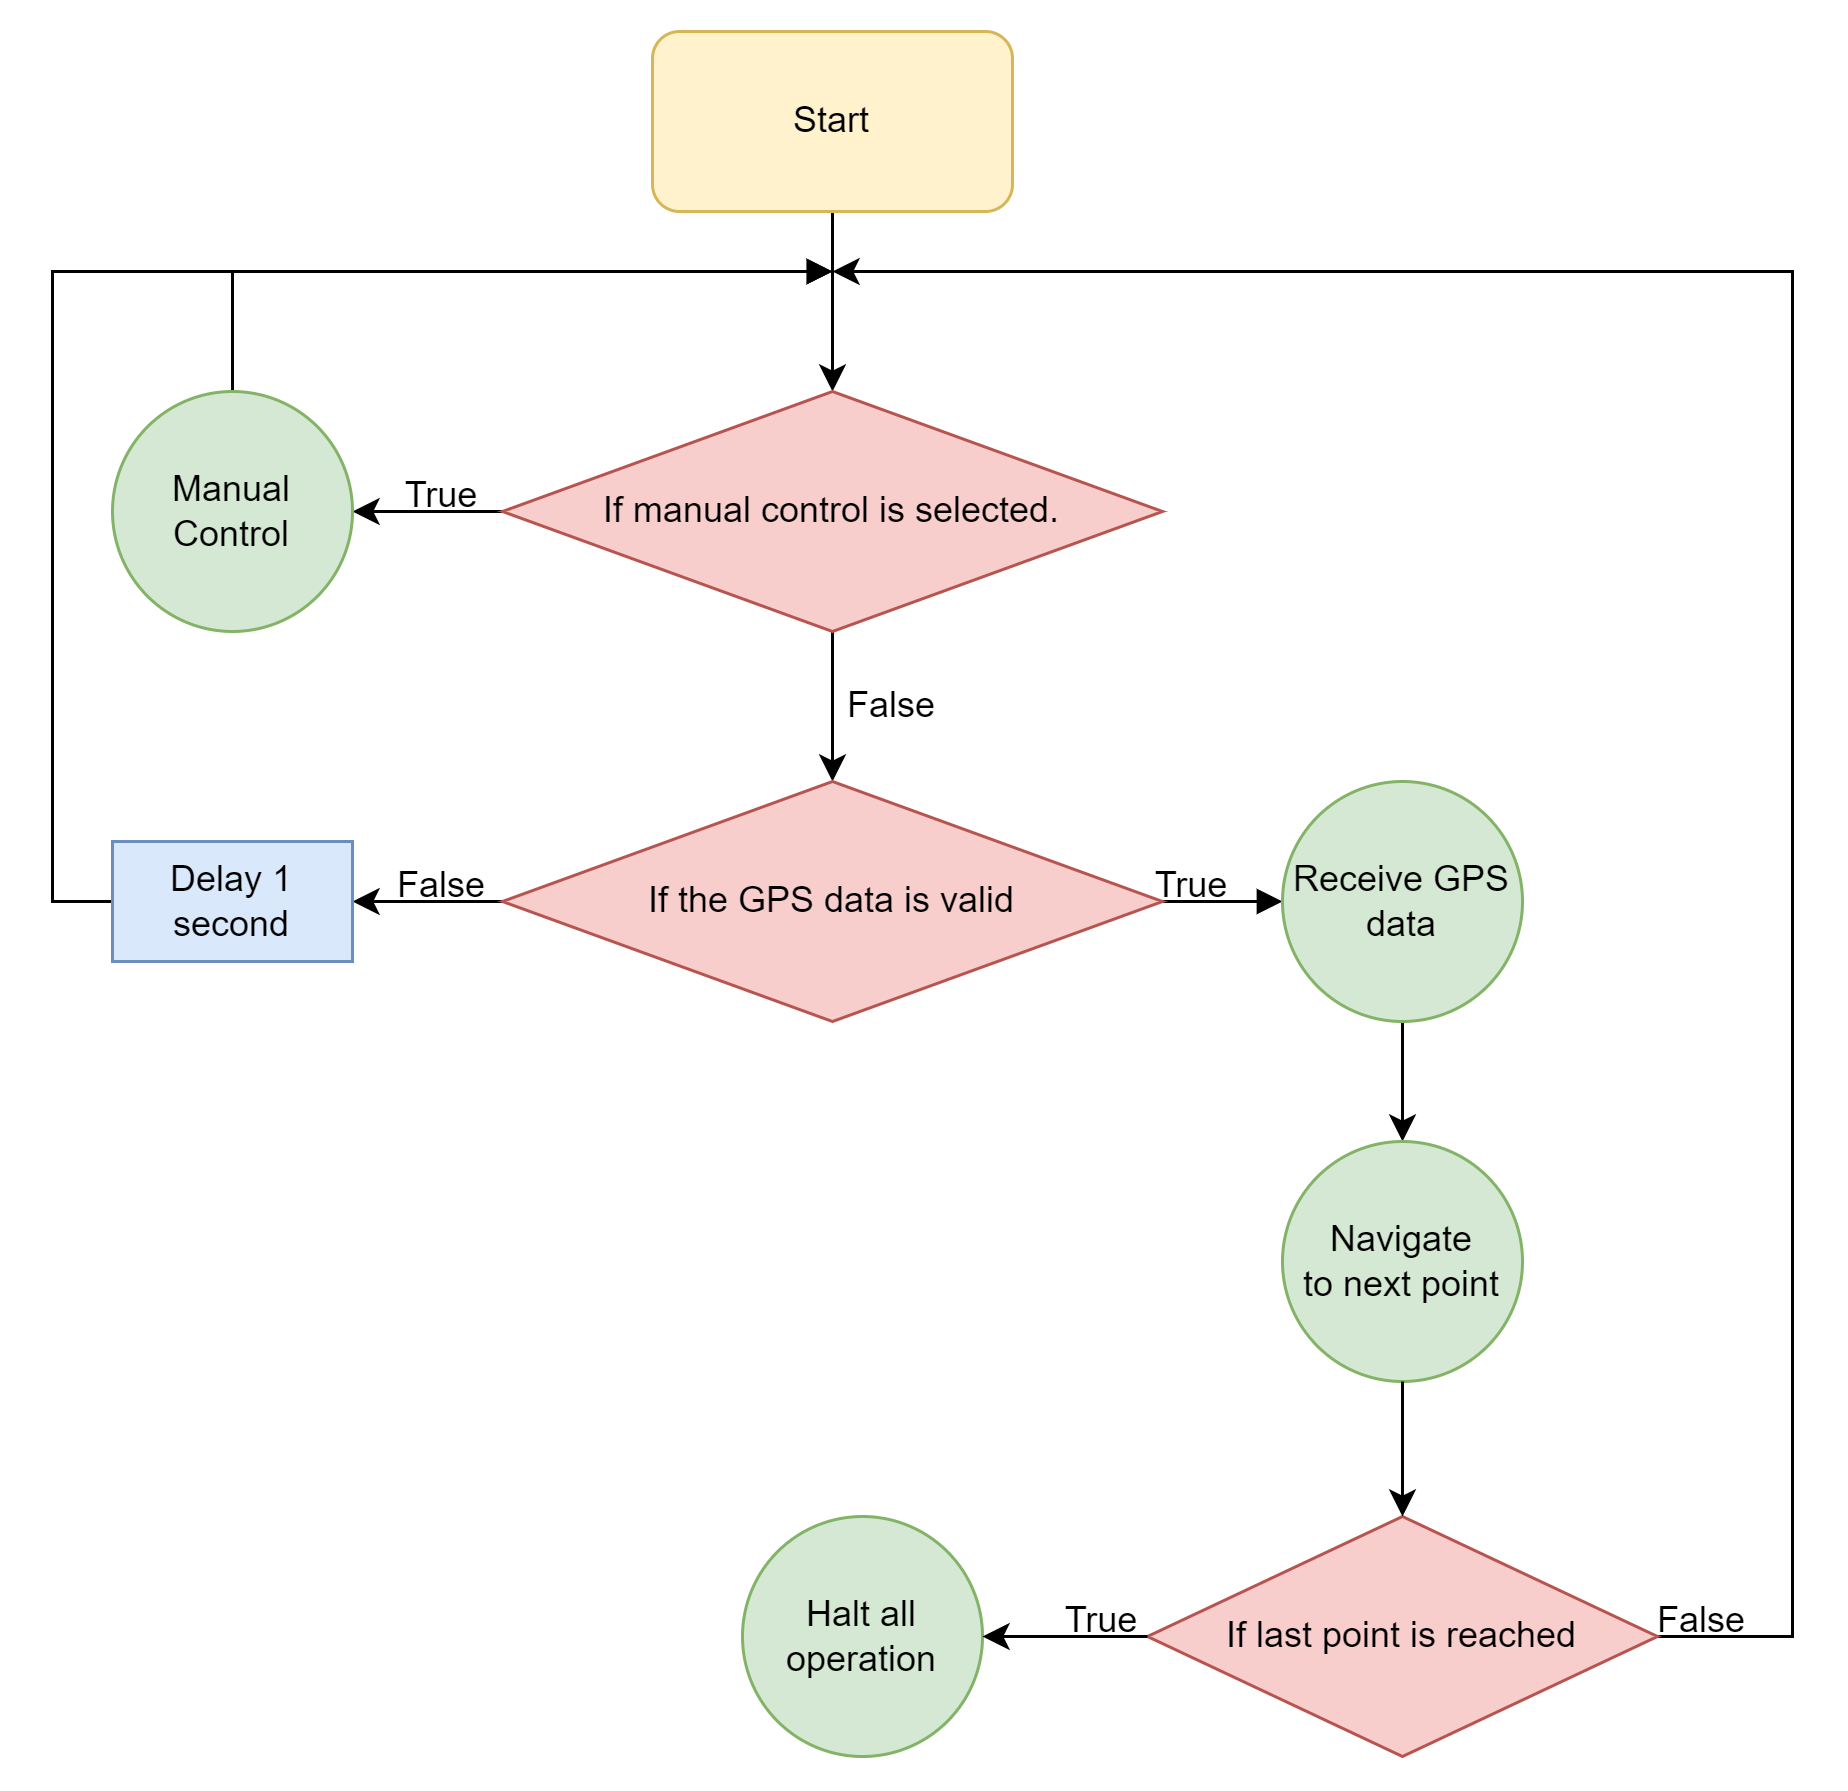
\includegraphics[width = 0.66\linewidth]{figures/statemachine.png}
			\caption{Flow diagram of the main states in the system.}
			\label{fig:3:stateMachine}
		\end{center}
	\end{figure}
		The system makes use of a state machine to switch between tasks. There are four different states in which the system can be, waiting for valid GPS, manual navigation, autonomous navigation and halt. Figure \ref{fig:3:stateMachine} shows the relationship between these states. The algorithm shown is executed in the main while loop of the microcontroller and shows one cycle. The loop starts by checking the user input. The user can select to switch between the manual and autonomous operation at any point. However, if autonomous navigation is selected and the GPS data is valid, the system will only enter manual control once the cycle has been completed. The psuedo code for this loop is shown in Algorithm \ref{alg:3:mainWhile}.
		
	
%The source code that will be discussed can be seen in Appendix \ref{Code}


\subsubsection{Manual Control}
The manual control involves receiving an input from the user and translating this to correctly power the thrusters. As seen in Algorithm \ref{alg:3:mainWhile}, the manual control involves the call of two functions: the first where most of the processing is done and the second is updating the RA register to produce the correct PWM signal. Firstly, the flow diagram of the first one, \emph{updatePWM()} is shown in Figure \ref{fig:3:updatePWM}. This shows the process to read one side's input and calculate the required duty cycle for that side's thruster. This is carried out for both sides in each cycle. As mentioned, the second function \emph{powerThruster()} simply writes the required value to RA register for the appropriate duty cycle. The psuedo for both functions are shown in the Algorthim \ref{alg:3:manualControl}.
\begin{figure}
	\begin{center}
		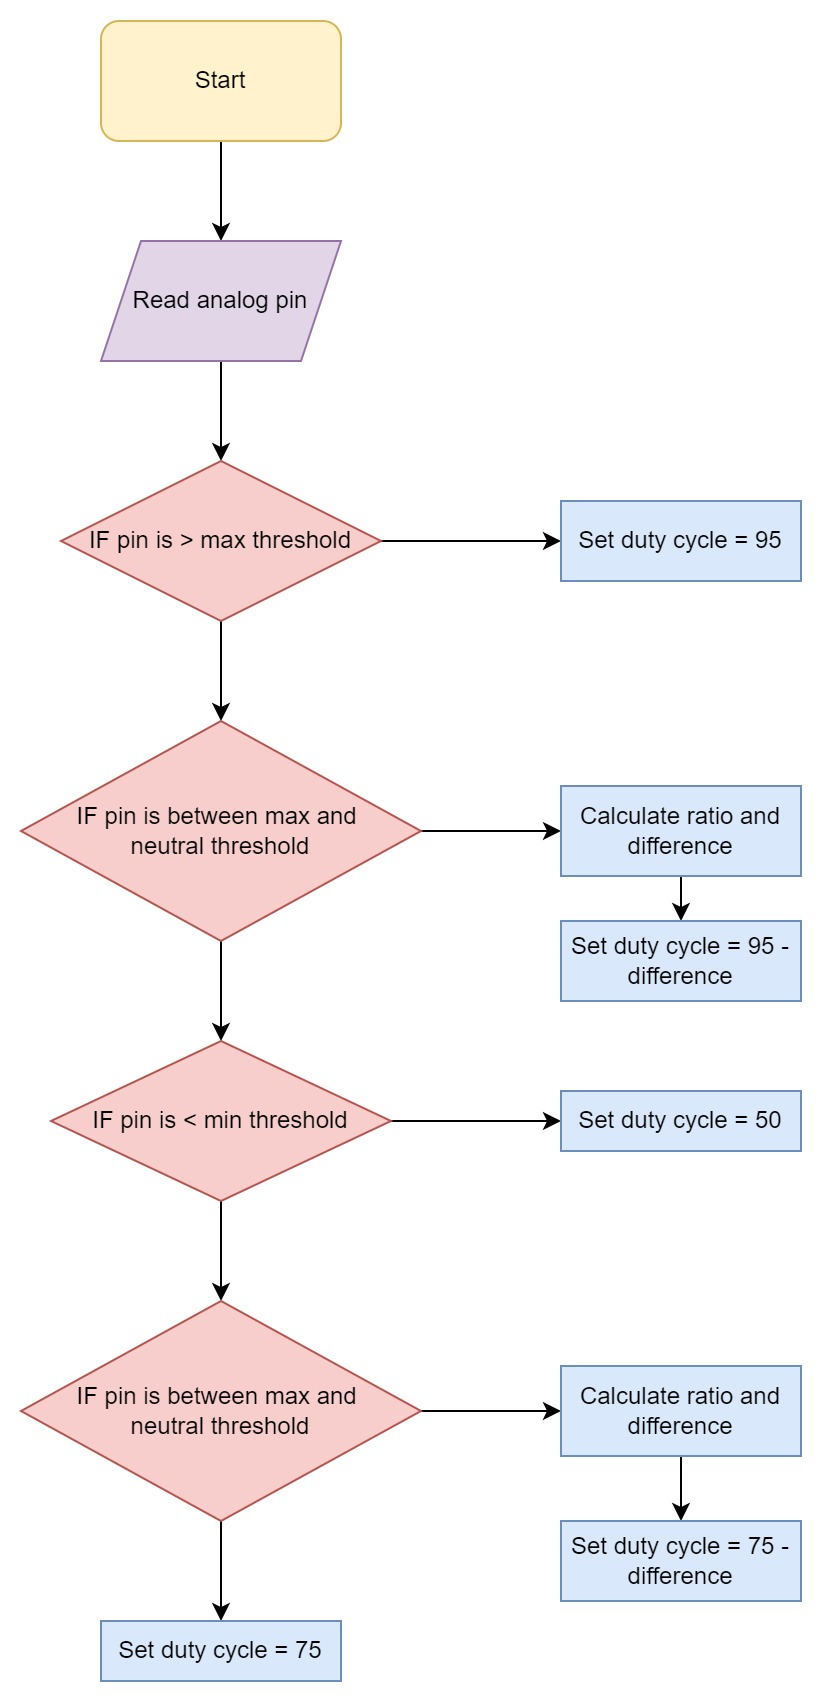
\includegraphics[width = 0.55\linewidth]{figures/UpdatePWM.jpg}
		\caption{Flow diagram of \emph{updatePWM().}}
		\label{fig:3:updatePWM}
	\end{center}
\end{figure}
\begin{algorithm}
	\caption{Pseudo code for manual control}
	\label{alg:3:manualControl}
	\begin{algorithmic}[1]
		\Procedure{updatePWM}{}
		\State $\textit{analog} \gets \textit{analogRead(analogPin)}$
		\If{$\textit{analog} > \textit{maximum threshold}$}
		\State $\textit{duty cycle} \gets 95$;
		\ElsIf{$\textit{analog}>\textit{neutral threshold}$}
		\State $\textit{analog ratio} \gets \textit{ratio forward (equ. \ref{eq:3:dutyF}) as } \textbf{float} $
		\State $\textit{difference} \gets (95 - 75) \times \textit{analog ratio as } \textbf{float}$
		\State $\textit{duty cycle} \gets 95 - \textit{difference} $
		\ElsIf{$\textit{analog} < \textit{minimum threshold} $}
		\State $\textit{duty cycle} \gets 50$;
		\ElsIf{$\textit{analog}<\textit{neutral threshold} $}
		\State $\textit{analog ratio} \gets \textit{ratio reverse (equ. \ref{eq:3:dutyR}) as }\textbf{float} $
		\State $\textit{difference} \gets (75 - 50) \times \textit{analog ratio as } \textbf{float}$
		\State $\textit{duty cycle} \gets 75 - \textit{difference}$
		\Else 
		\State $\textit{duty cycle} \gets 75$;
		\EndIf
		\EndProcedure
		\Procedure{powerThrusters}{}
		\State $\textit{RA} \gets \textit{RC} \times \textit{duty cycle\SI{}{\percent}}$;
		\EndProcedure
	\end{algorithmic}
\end{algorithm}
\subsubsection{Receiving GPS Data}
The GPS data is received with serial UART communication and is a string of characters as shown previously. To receive the correct data line, the microcontroller receives each line and then checks that it is the required line. Given the required line, the line is processed and the struct is updated with the newest data. A few small tools were written to assist in this. They are all relatively simple and so their pseudo is unnecessary but a brief description follows for context.\par
\textbf{findAllInstacesOf()}\par
This function takes an integer array, a character array to search, a character to search for and the size of the character array to search as parameters. It returns the integer array with the index positions of the character searched for.\par
\textbf{charToInteger()}\par
This function takes a character array and a start and end index as integers. It returns an integer as it would be seen as the character string. For example, the character string '4862' would be returned as 4862 as an integer.\par
\textbf{charToDecimals()}\par
This function is similar to the integer version but it returns a float with the numbers as the decimals. For example a character string of '4862' would be returned as 0.4862.\par
The overall process to receive the GPS data and populate the struct is shown in the flow diagram of Figure \ref{fig:3:recGPS}. The struct is populated by using the two arrays, containing indexes full stops and commas indexes withing the character array, to split up the character array into the necessary information. This is easily done as the string from the GPS has a standard form.
\begin{algorithm}
	\caption{Pseudo code for receiving GPS data}
	\label{alg:3:receiveGPS}
	\begin{algorithmic}[1]
		\State $\textit{msgReceived} \gets \textit{false}$
		\State $\textit{rxCnt} \gets 0$
		\While{$!\textit{msgRecieved}$}
		\While{$ \textit{rxByte} != 10$}
		\State $\textit{rxByte} \gets \textit{SerialRead()}$
		\If{$\textit{rxByte} != -1$}
		\State $\textit{rxData(rxCnt)} \gets \textit{rxByte}$
		\State $\textit{rxCnt} \gets \textit{rxCnt} + 1$ 
		\EndIf
		\EndWhile
		\If{$\textit{rxData(3) = \textit{'R' AND rxData(4)} = \textit{'M' AND rxData(5)} = \textit{'C'}}$}
		\State $\textit{call updateStructRMC(rxData, rxCnt)}$
		\State $\textit{msgReceived} \gets \textit{true}$
		\EndIf
		\State $\textit{rxCnt} \gets 0$
		\State $\textit{rxByte} \gets 0$
		\EndWhile
	\end{algorithmic}
\end{algorithm}
\begin{figure}[!hb]
	\begin{center}
		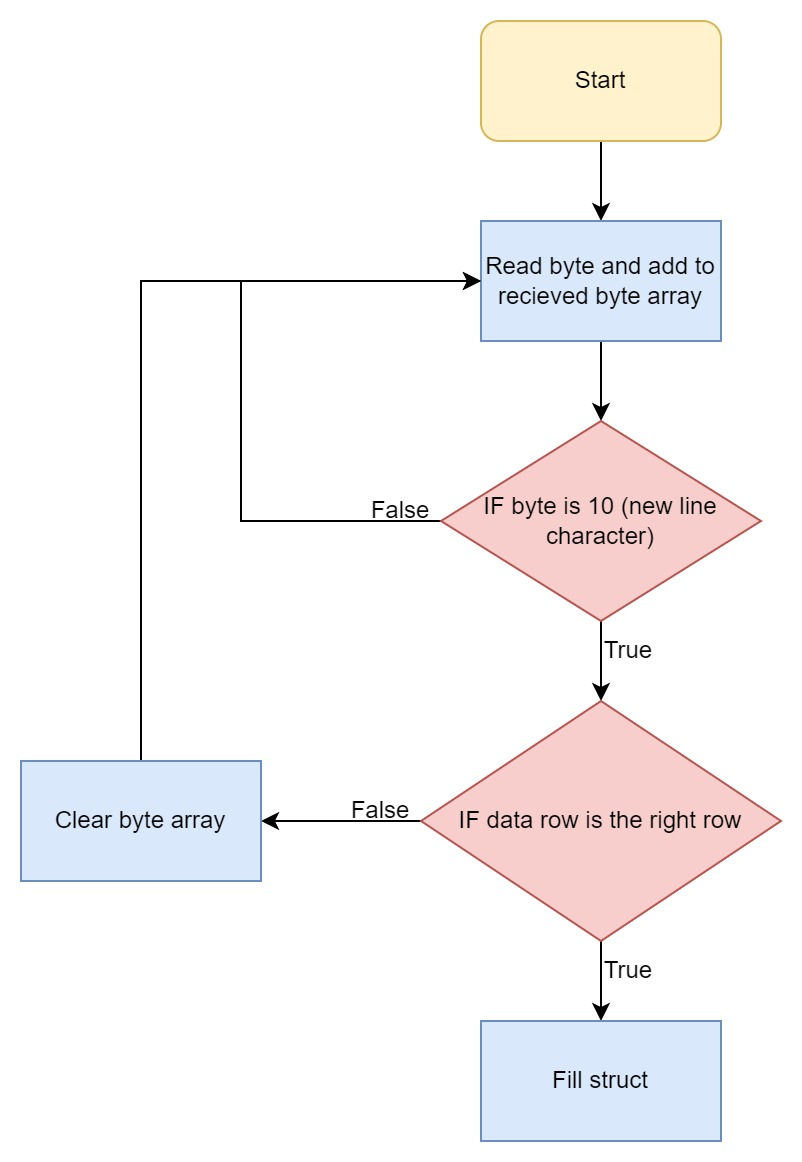
\includegraphics[width = 0.35\linewidth]{figures/receiveGPS}
		\caption{The flow diagram of receiving the GPS data.}
		\label{fig:3:recGPS}
	\end{center}
\end{figure}
\subsubsection{Autonomous Navigation}
The autonomous navigation will only begin executing when valid GPS data has been received. Therefore, there is no need to check the data when the navigation algorithm begins. The target points for the navigation are written into a text file prior to launching. The program reads these points into a struct at the start of operation to be ready for the autonomous navigation. The autonomous control calculates the distance and bearing to its destination and the error between its current bearing and its target bearing. To calculate the distance between two points that are very close together, one can use Pythagoras theorem without much error because across a small instantaneous distance the world is flat. However, due to the curvature of the earth, across much larger distances the Pythagoras theorem looses accuracy. Therefore in this project the haver-sine formula, equations \ref{equ:3:a} - \ref{equ:3:d}, is used where $\phi$ is latitude and $\lambda$ is longitude, both in radians. Furthermore, the curvature of the earth effects the bearing along the line between two points. Therefore, the bearing to target calculated in this project is the forward azimuth as this is the bearing that if followed on a straight line along the arc of the earth would lead to the final point. \cite{VanBrummelen2013}, \cite{Veness2002}, \cite{Alger1910}\par
\begin{equation}
	a = \sin{(\frac{\triangle\phi}{2})}^2 + \cos{\phi_{1}}\times\cos{\phi_{2}}\times\sin{(\frac{\triangle\lambda}{2})}^2
	\label{equ:3:a}
\end{equation}
\begin{equation}
	c = 2\times\arctan2(\sqrt{a}, \sqrt{1-a})
\end{equation}
\begin{equation}
	d = 6371000 \times c
	\label{equ:3:d}
\end{equation}
If the distance and bearing error are above a set threshold, the system will move at full power using full steering. However, once it is within the distance threshold, it will begin to slow down proportional to how close it is. The amount of throttle as a percentage is determined by a ratio of the remaining distance and the distance threshold. Furthermore, once the distance is reduced below the arrival threshold, the point is marked as 'passed' and the system will begin navigating to the next point or halt operation if there are no more points. Similarly for the steering, the amount of steering as a percentage is a ratio of the bearing error and the steering threshold. Finally, the direction to steer in is determined using an equation that accounts for the \SI{360}{\degree}/\SI{0}{\degree} turnover point. If the target bearing is anywhere within \SI{180}{\degree} to the right of the current bearing, it will turn right and visa versa. This logic and pseudo code can be seen in the flow diagram of Figure \ref{fig:3:autoNav} and Algorithm \ref{alg:3:autoNav}. In the pseudo code only the procedure for \emph{steerLeft()} is shown as the procedure for \emph{steerRight()} follows the exact same logic but with the thruster sides inverted. 

\begin{figure}
	\begin{center}
		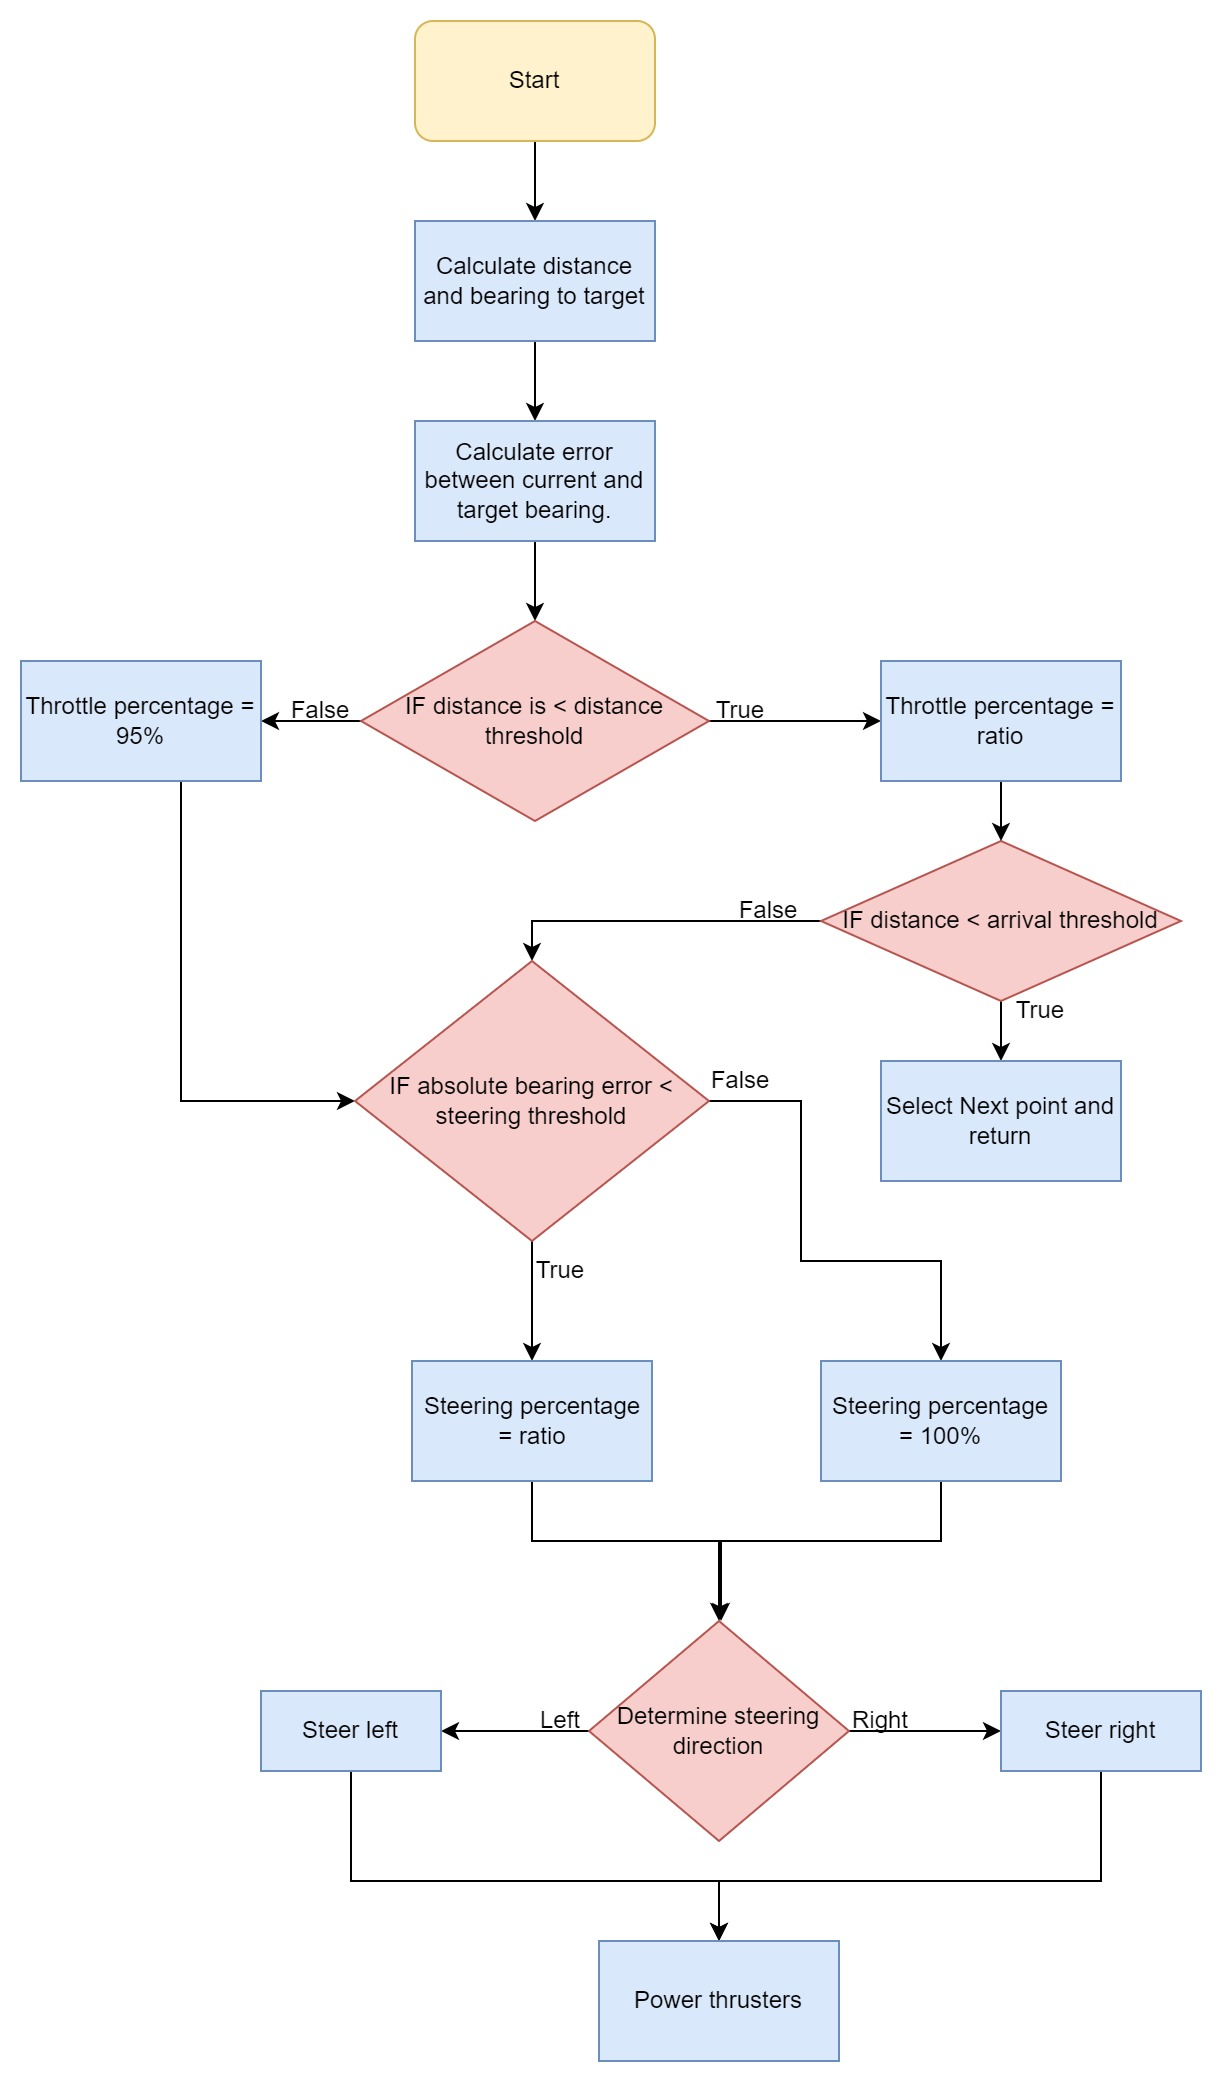
\includegraphics[width=0.7\linewidth]{figures/autoNav.jpg}
		\caption{Flow diagram of the autonomous navigation}
		\label{fig:3:autoNav}
	\end{center}
\end{figure}
\begin{algorithm}
	\caption{Pseudo code for the autonomous navigation}
	\label{alg:3:autoNav}
	\begin{algorithmic}[1]
		\Require{Read the target GPS points from SD card.}
		\Procedure{navigate()}{}
		\State $\textit{Calculate distance to target}$
		\State $\textit{Calculate bearing to target}$
		\State $\textit{Calculate the error between current and target bearing}$
		\If{$\textit{distance} < \textit{distance threshold}$}
		\State $\textit{throttle percentage} \gets \frac{\textit{distance}}{2 \times \textit{distance threshold}} $
		\If{$\textit{distance} < \textit{arrival threshold}$}
		\State $\textit{call NextPoint()}$
		\State $\textbf{return}$
		\EndIf
		\Else 
		\State $\textit{throttle percentage} \gets 95$
		\EndIf
		\If{$\textit{abs(bearing error)} < \textit{steering threshold}$}
		\State $\textit{steering percentage} \gets \frac{\textit{abs(bearing error)}}{\textit{steering threshold}}$
		\Else
		\State $\textit{steering percentage} \gets 100$
		\EndIf
		\State $\textit{maxBearing} \gets \textit{max(bearing error, target bearing)}$
		\State $\textit{minBearing} \gets \textit{min(bearing error, target bearing)}$
		\If{$(\textit{maxBearing = target bearing}) \textit{XOR} (\textit{maxBearing} - \textit{minBearing}) >180 )$}
		\State $\textit{call steerLeft()}$
		\Else
		\State $\textit{call steerRight()}$
		\EndIf
		\State $\textit{call powerThrusters()}$
		\EndProcedure
		\Procedure{NextPoint()}{}
		\State $\textit{points(targetIndex).passed} \gets \textit{true}$
		\State $\textit{targetIndex} \gets \textit{targetIndex} + 1$
		\If{$\textit{points.targetIndex does not exists}$}
		\State $\textit{state} \gets \textit{Halt navigation}$
		\EndIf
		\EndProcedure
		\Procedure{steerLeft()}{}
		\State $\textit{throttle difference} = 2 \times \textit{throttle percentage}$
		\State $\textit{rightSide.duty Cycle} \gets 75 + (25 \times (\textit{throttle percentage}\SI{}{\percent}))$
		\State $\textit{leftSide.duty Cycle} \gets \textit{rightSide.duty Cycle} - (25 \times ((\textit{throttle difference} \times (\textit{steering percentage}\SI{}{\percent}))/100))$
		\EndProcedure
	\end{algorithmic}
\end{algorithm}
\chapter{Testing and Results}
In order to test the system a series of tests were conducted to test each system individually before the overall system was tested. The individual systems tested are the GPS and compass, the PWM output, throttle, and the individual thrusters. Finally the full system was tested on the Stellenbosch canoe dam. 
\section{GPS and Compass}
The GPS and compass were tested on land. A baseline was established using a tracking application on a cellphone. The GPS and compass together with the cellphone were placed in a bag and a route was walked. The tracking data from both sources can then be downloaded and formatted as a Keyhole Markup Language (.kml) file and displayed on a map or plotted as has been done in figure \ref{fig:4:GPSMap}.\par
\begin{figure}
	\begin{center}
		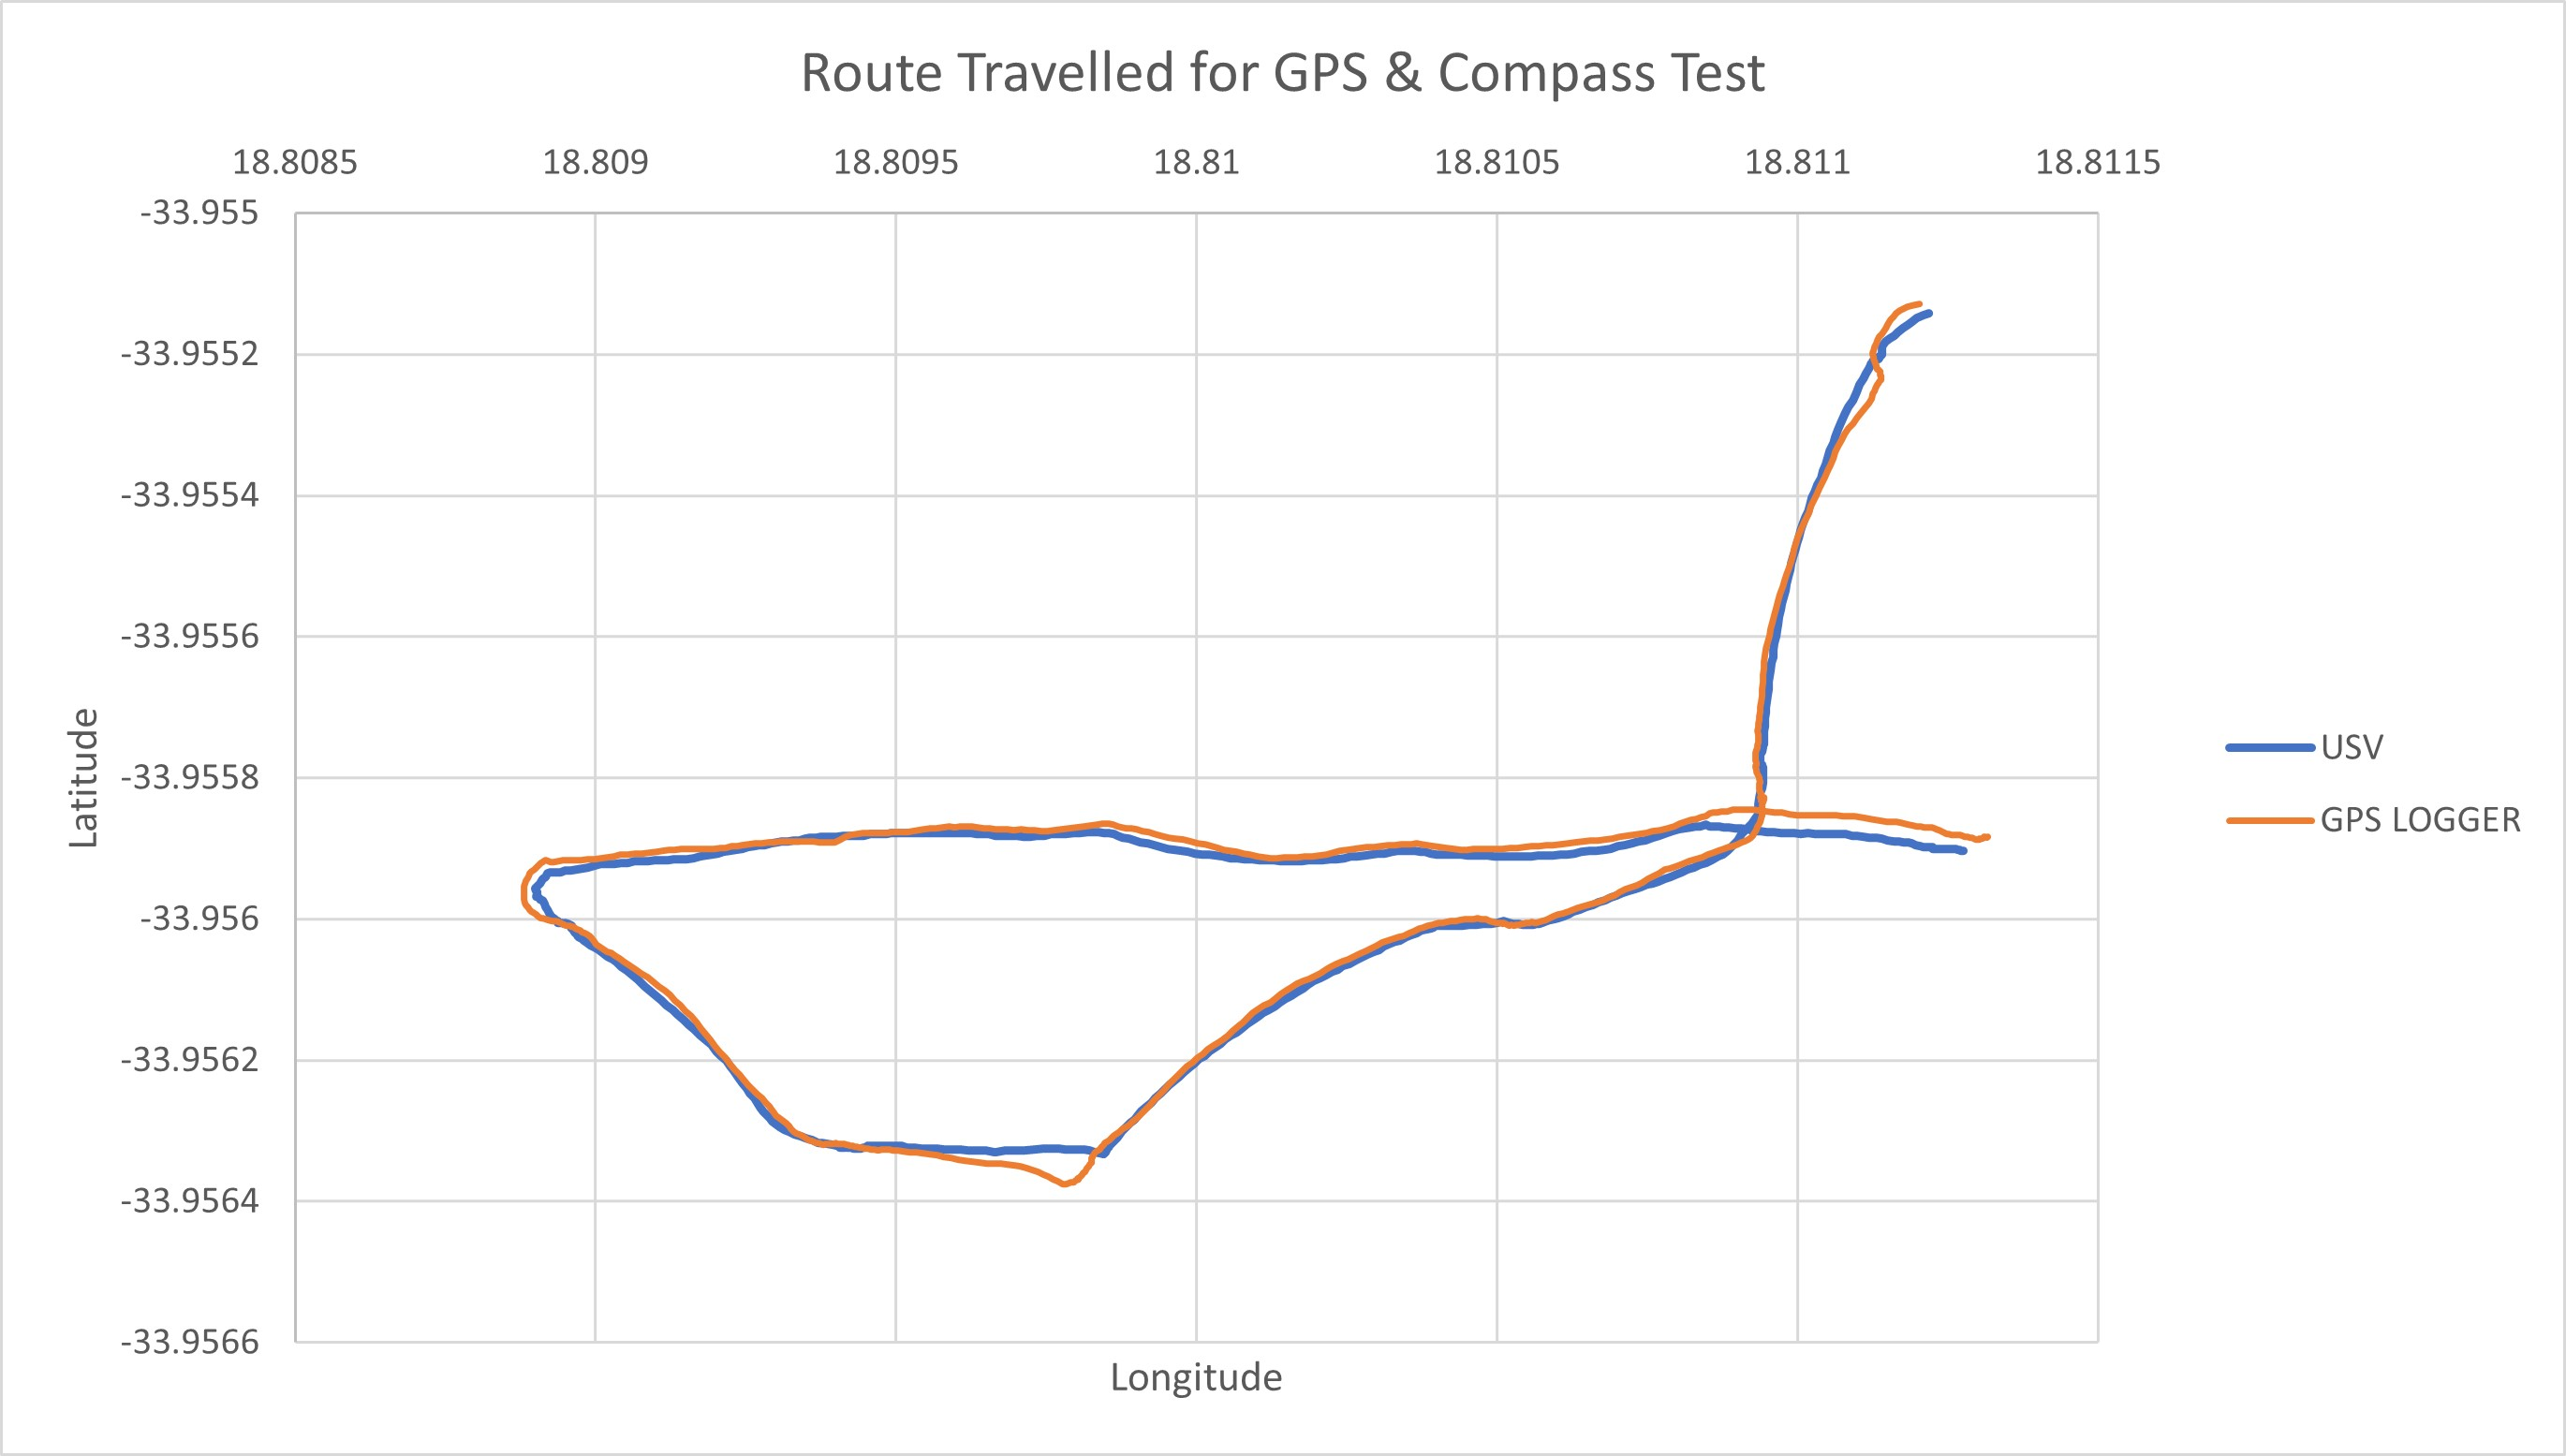
\includegraphics[width=0.8\linewidth]{figures/graphGPSMap.jpg}
		\caption{The path used to compare the system GPS and the baseline GPS logger.}
		\label{fig:4:GPSMap}
	\end{center}
\end{figure}
In order to have a bearing to compare the compass reading with, the last two GPS points were used to calculate the bearin on which the vessel is pointing. Figure \ref{fig:4:bearingTest} shows the calculated bearing and the GPS bearing plotted together.\par
\begin{figure}
	\begin{center}
		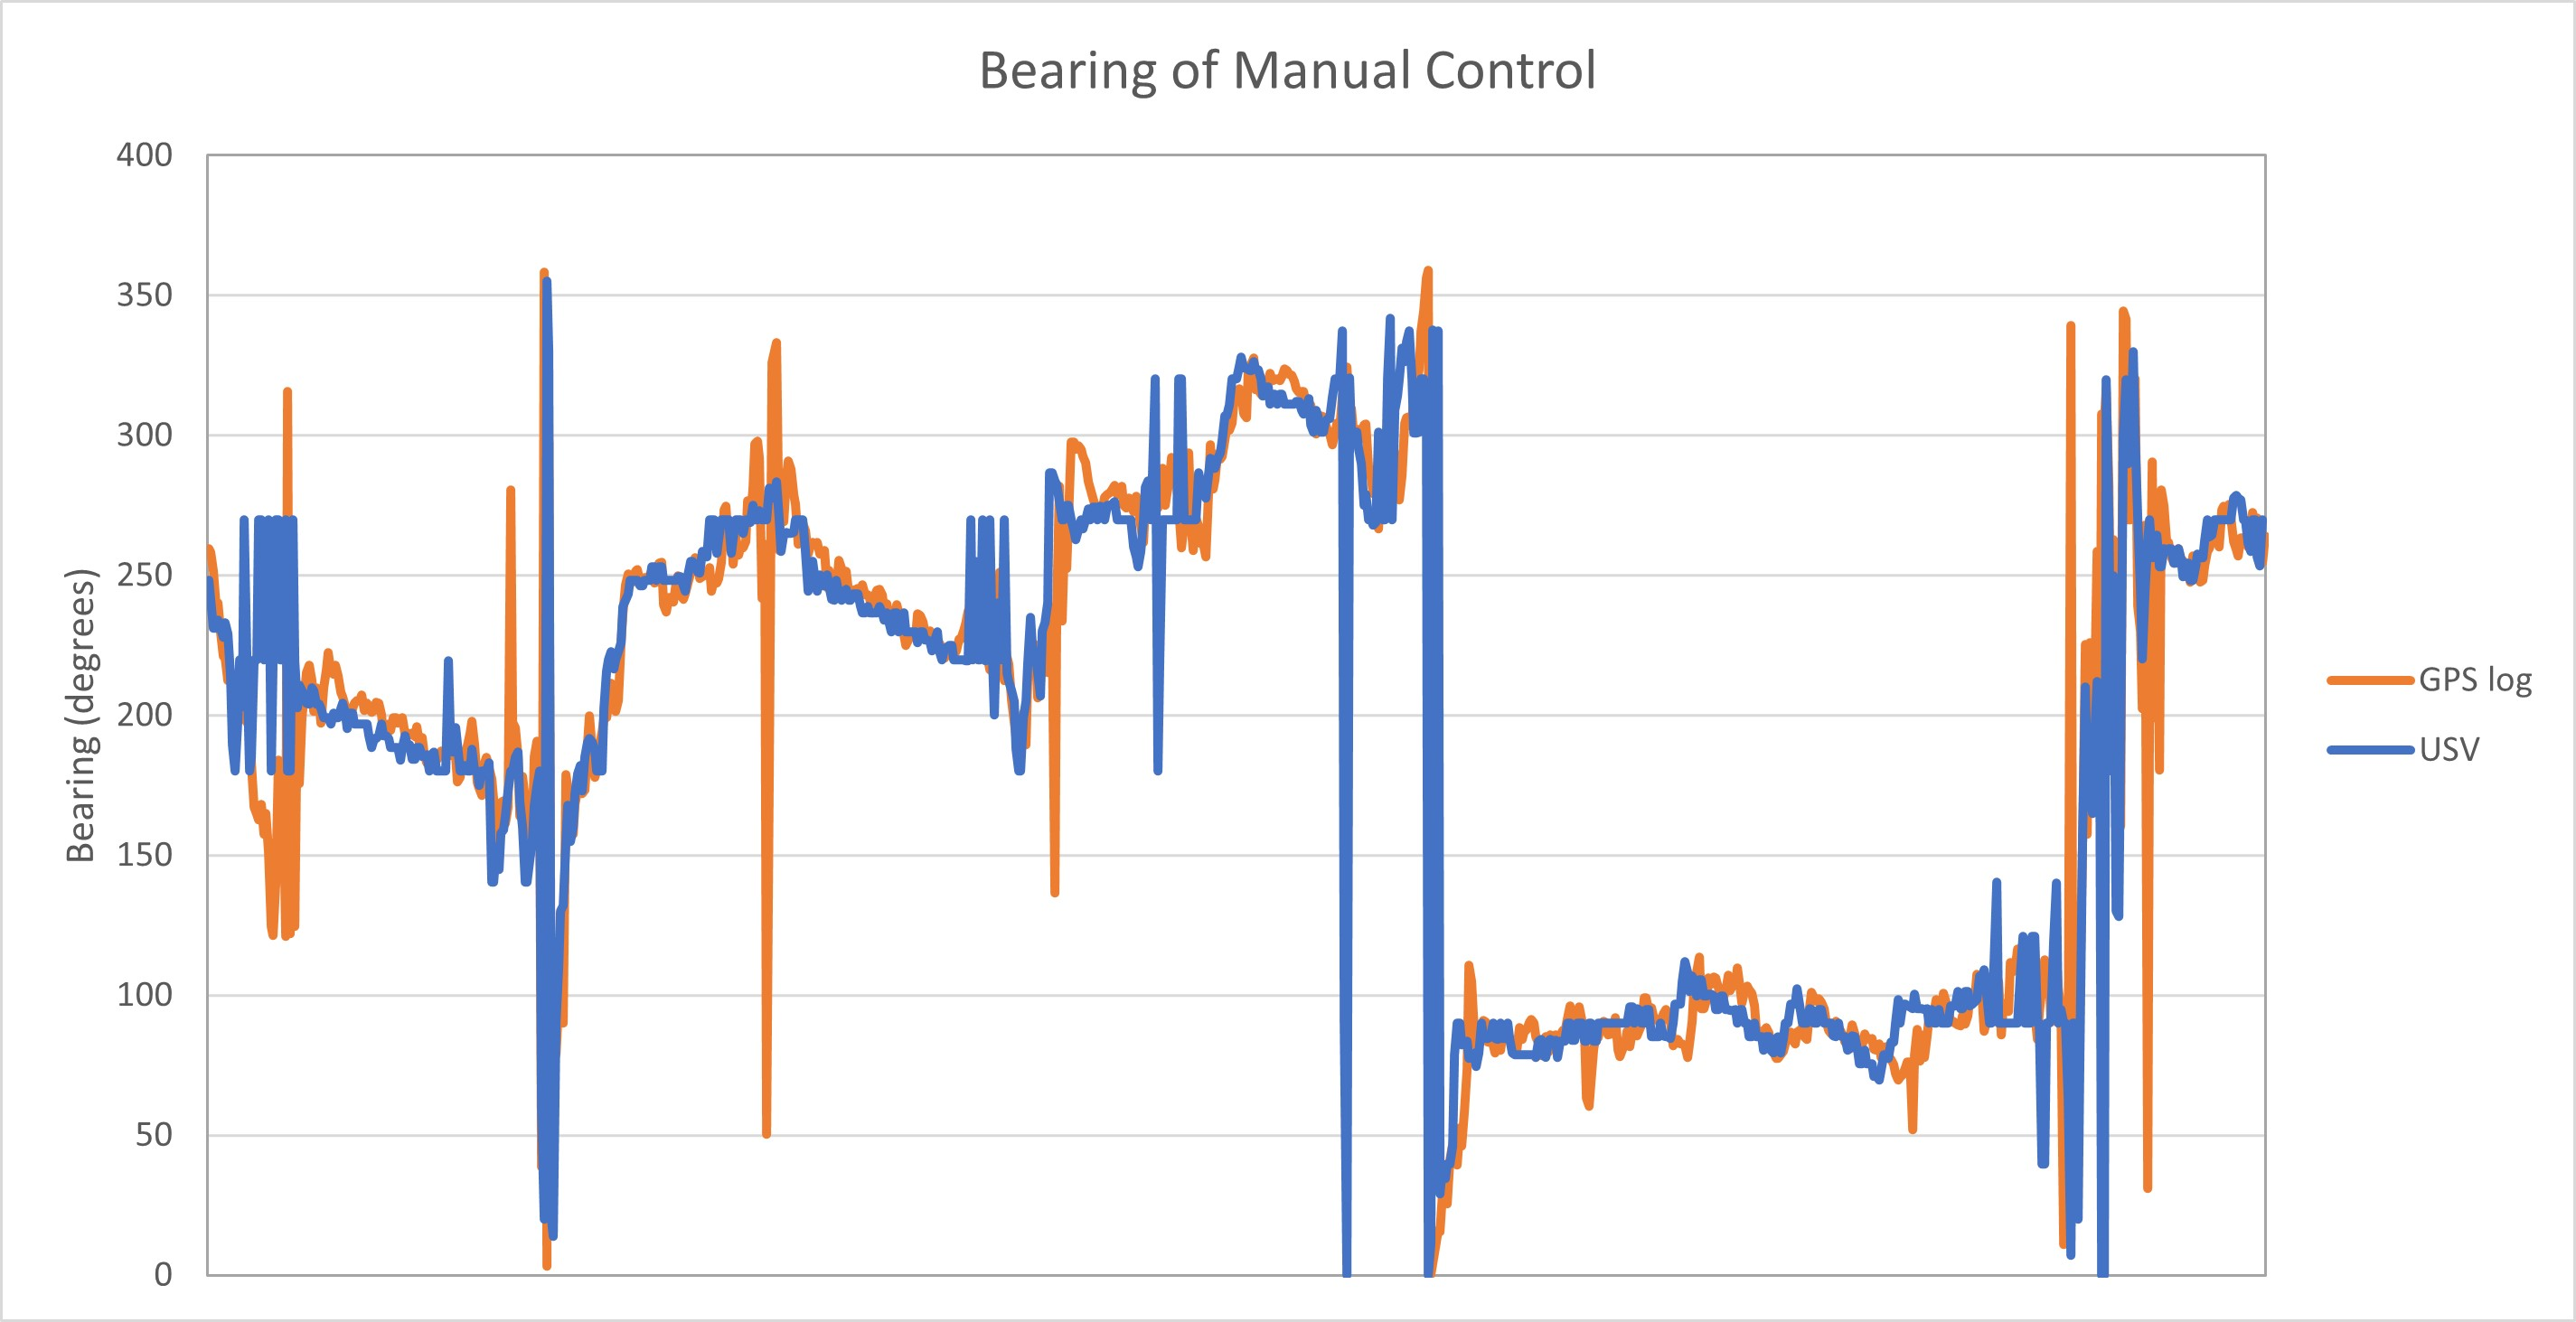
\includegraphics[width=0.8\linewidth]{figures/graphBearingManual.jpg}
		\caption{The calculated bearing and compass bearing overlay.}
		\label{fig:4:bearingTest}
	\end{center}
\end{figure}
As can be seen in figure \ref{fig:4:GPSMap}, the two sets of GPS data match each other very closely with only a few areas where the systems GPS moves away from the baseline GPS points. In order to quantify the accuracy of the GPS, the distance between the coinciding points of the baseline GPS and the system GPS was calculated and plotted on box and whisker chart of figure \ref{fig:4:GpsBxWh}. As you can see the GPS is accurate to within \SI{5}{\meter} with only a few outliers, making up less than \SI{4}{\percent} of the data, falling slightly outside the \SI{5}{\meter} mark.\par
Similarly it can be seen on figure \ref{fig:4:bearingTest} that the systems compass bearing is closely following the calculated baseline bearing. Figure \ref{fig:4:bearingBxWh} shows a box and whisker plot of the error between the two bearings, with most of the data falling within a \SI{20}{\degree} range. There are more outliers than in the GPS test, however this is due to calculated bearing having several spikes. These spikes occur when the because the bearing is being calculated between GPS points that are often within 1m of each other and some accuracy can be lost. The noticeable spike of the system compass in figure \ref{fig:4:bearingTest} is not an error but caused by the bearing going around passed \SI{360}{\degree} to \SI{0}{\degree}.
 \begin{figure}[!hb]
 	\begin{center}
 		\begin{subfigure}{0.45\linewidth}
 			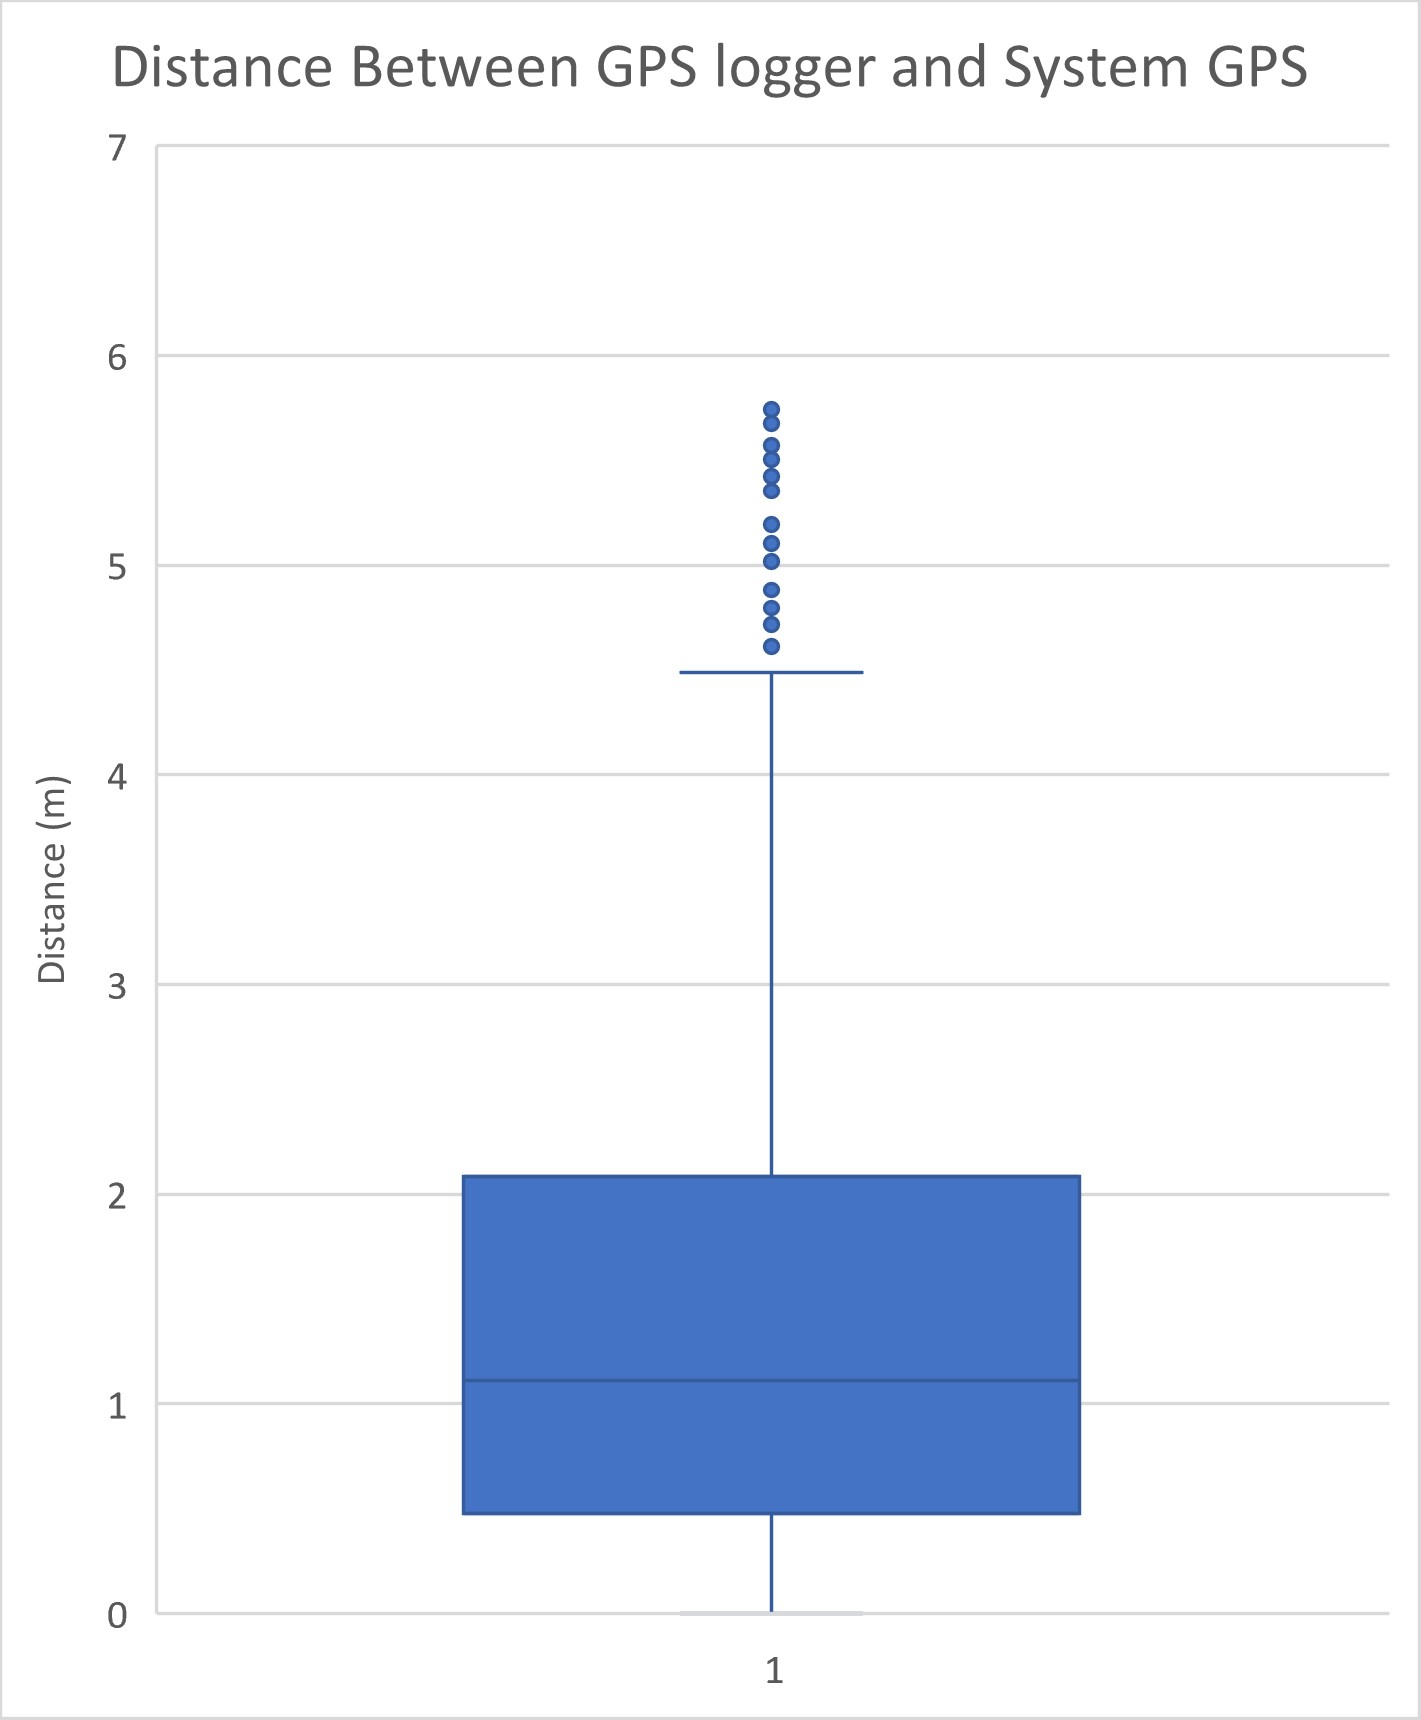
\includegraphics[width = \linewidth]{figures/distBxWh.jpg}
 			\caption{Distance.}
 			\label{fig:4:GpsBxWh}	
 		\end{subfigure}
 		\begin{subfigure}{0.475\linewidth}
 			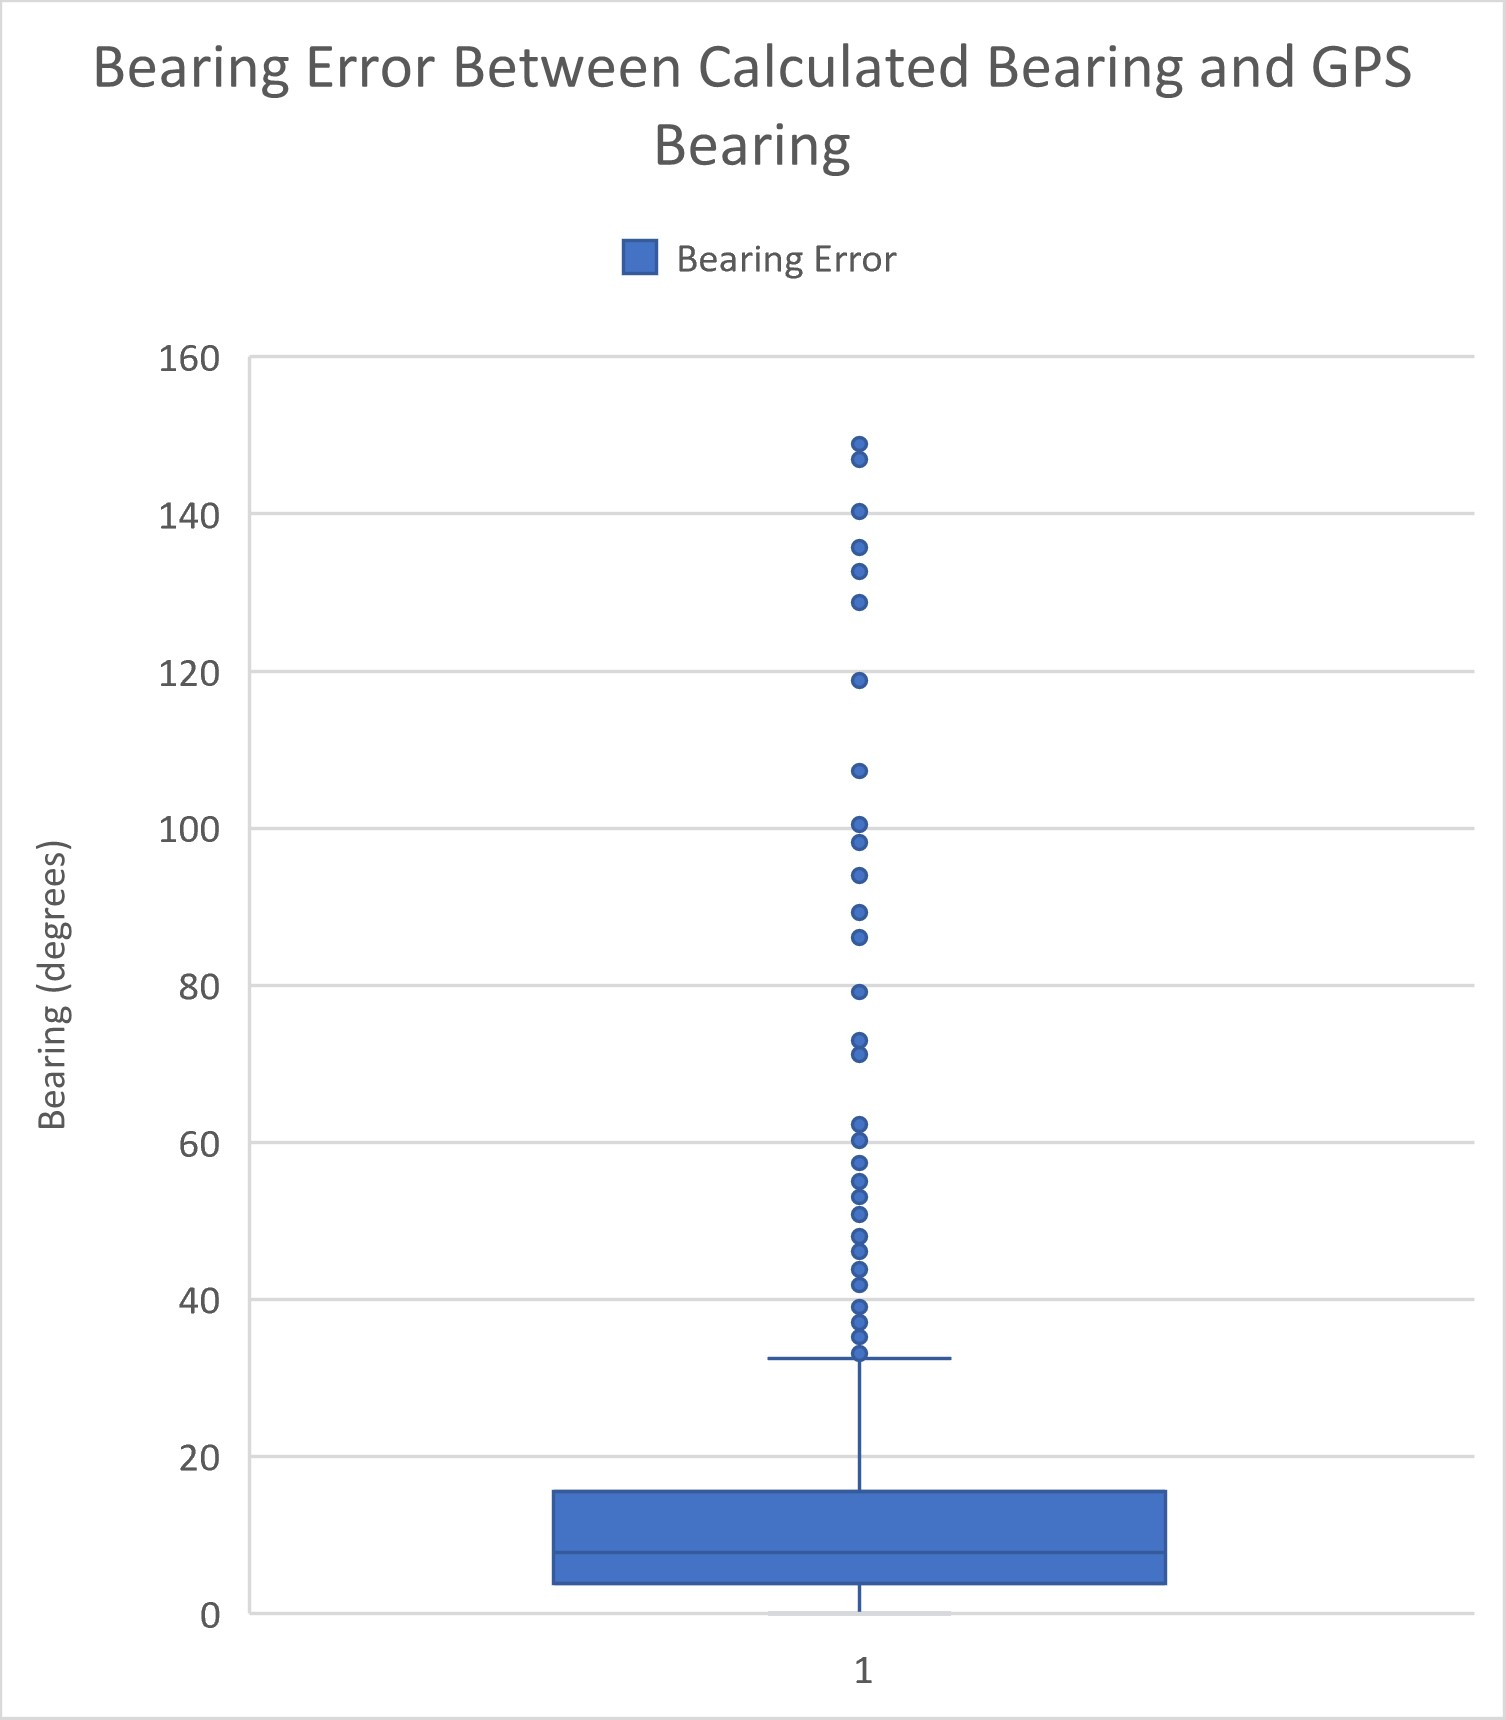
\includegraphics[width = \linewidth]{figures/bearingBxWh.jpg}
 			\caption{Bearing}
 			\label{fig:4:bearingBxWh}	
 		\end{subfigure}
 	\caption{Box and Whisker Graphs Of Distance and Bearing Between the System and the Baseline.}
 	\end{center}
 \end{figure} 
\section{PWM Output}
In order to adjust the speed of the thrusters, the PWM output must vary based on the throttle input. The PWM signal can easily be measured using an oscilloscope, therefore the system was set-up as shown in figure \ref{fig:4:PWMTest}. The throttle was connected to microcontrollers analogue inputs as it would be for the full system. The PWM outputs where then attached to the oscilloscope probes and the Arduino native programming port was used to power the system from a laptop. Each PWM signal was first tested individually before finally, both signals were tested simultaneously, each one on its own channel. \par
\begin{figure}
	\begin{center}
		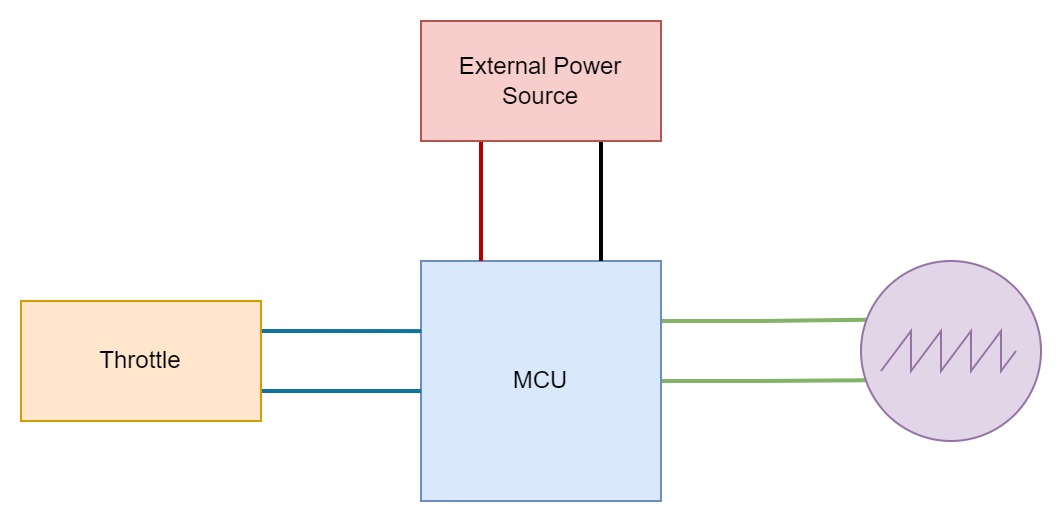
\includegraphics[width=0.6\linewidth]{figures/PWMtest.jpg}
		\caption{Wiring diagram for the PWM oscilloscope test.}
		\label{fig:4:PWMTest}
	\end{center}
\end{figure}
As the throttle is adjusted the PWM signal should vary. There are three distinct positions, full forward, neutral and full reverse. that can be noted in table \ref{tab:3:PWM}. Theses three positions were tested to ensure that the range of the throttle was correctly calibrated. Finally the PWM signal was observed while slowly adjusting the throttle to ensure that the PWM signal varied linearly and in with a timely response. The results of the oscilloscope test are shown in figure \ref{fig:4:OscTest}. \par
It can be seen that the PWM responded well to the throttle inputs and met all three of the notable positions perfectly. Figure \ref{fig:4:OscTest:both} also shows that the two PWM outputs can have independent values to control each thruster as required. It should be noted that the images in figure \ref{fig:4:OscTest} all show a amplitude of \SI{3.3}{\volt} as the output was measured directly off of the Arduino microcontroller and before the signal was amplified using the logic level converter. It was confirmed that the converter accurately amplified the signal while maintaining the frequency and duty cycle of the signal.
\begin{figure}
	\begin{center}
		\begin{subfigure}{0.47\linewidth}
			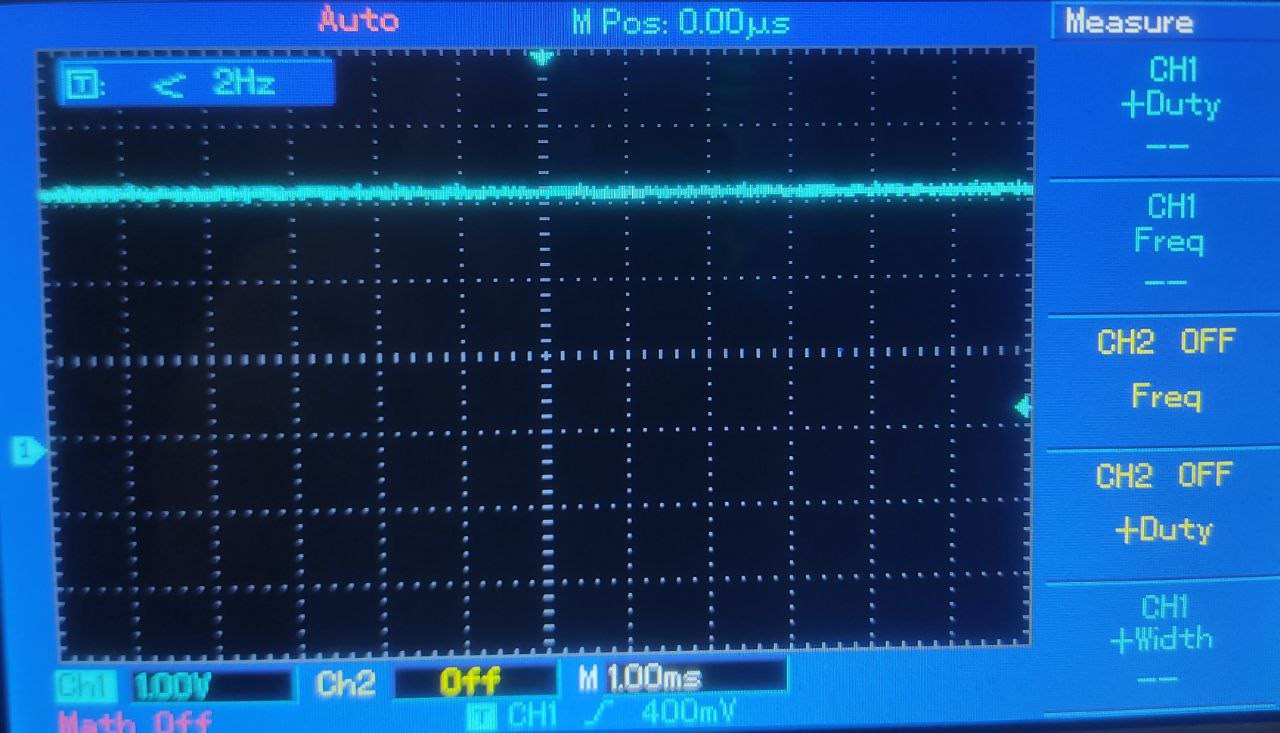
\includegraphics[width = \linewidth]{figures/PWMfoward.jpg}
			\caption{Full Forward}
			\label{fig:4:OscTest:forward}	
		\end{subfigure}
		\begin{subfigure}{0.47\linewidth}
			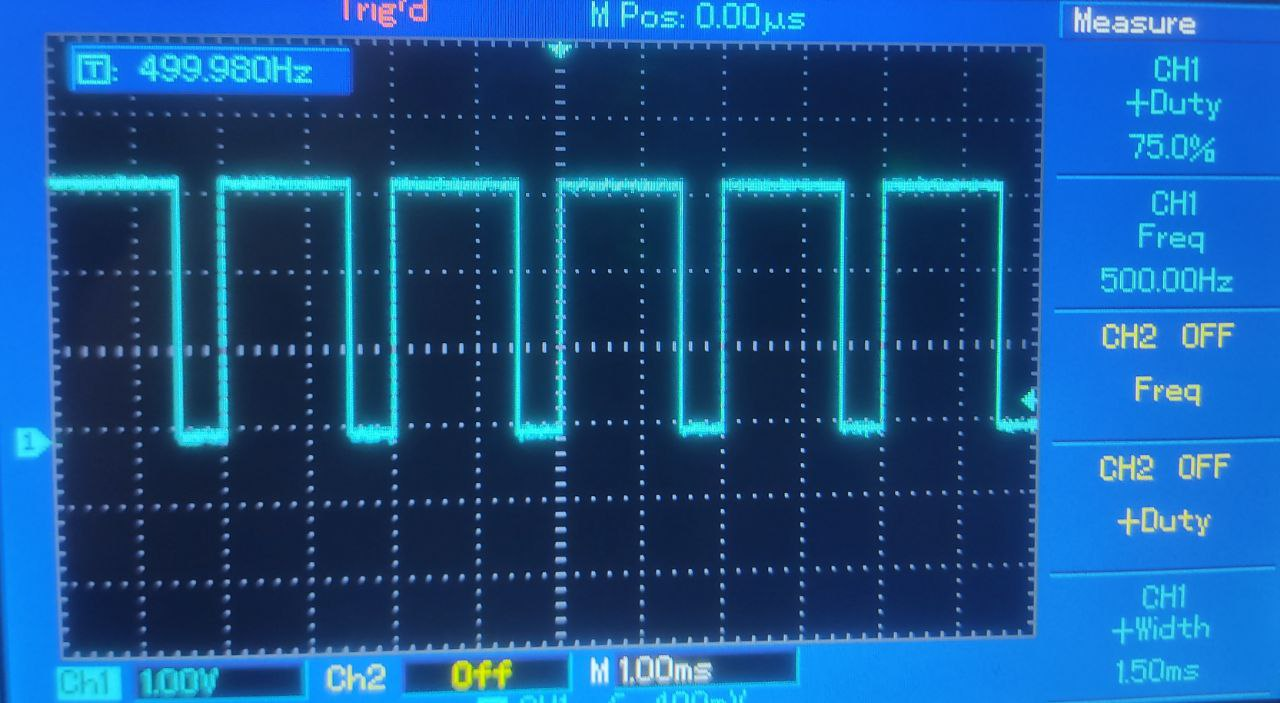
\includegraphics[width = \linewidth]{figures/PWMneutral.jpg}
			\caption{Neutral}
			\label{fig:4:OscTest:neutral}	
		\end{subfigure}
		\begin{subfigure}{0.47\linewidth}
			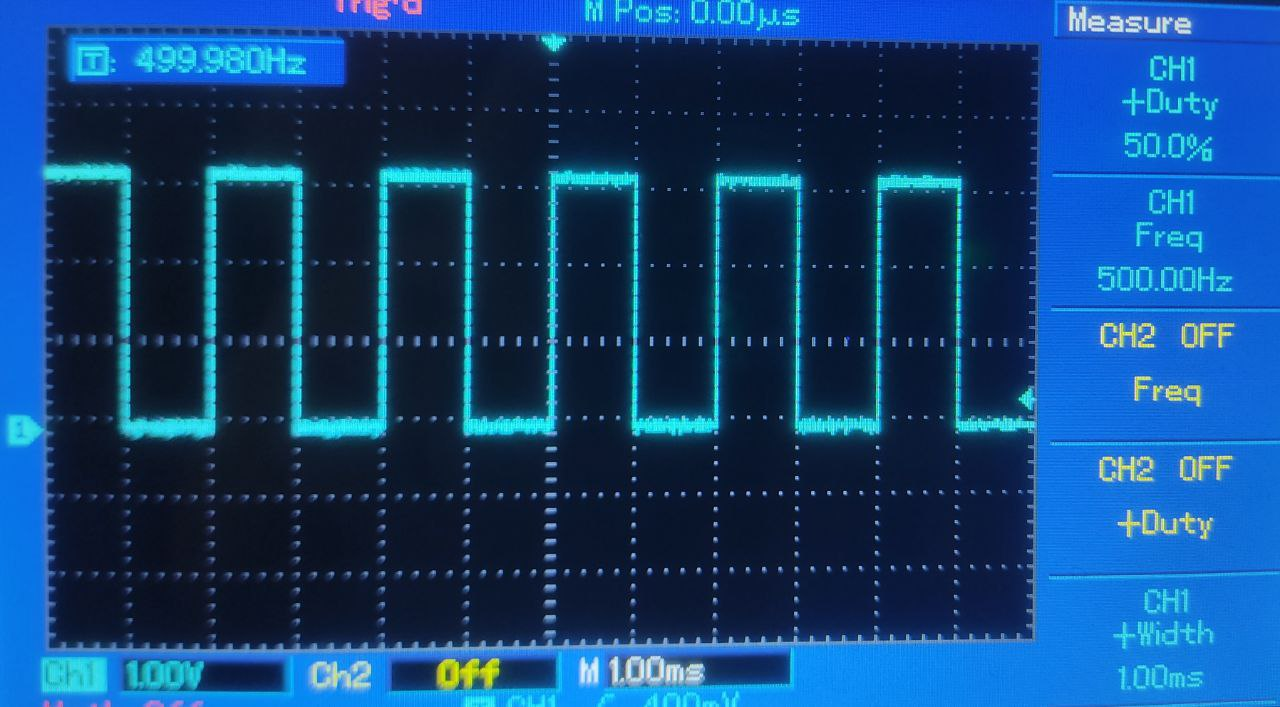
\includegraphics[width = \linewidth]{figures/PWMreverse.jpg}
			\caption{Full Reverse}
			\label{fig:4:OscTest:reverse}	
		\end{subfigure}
		\begin{subfigure}{0.47\linewidth}
			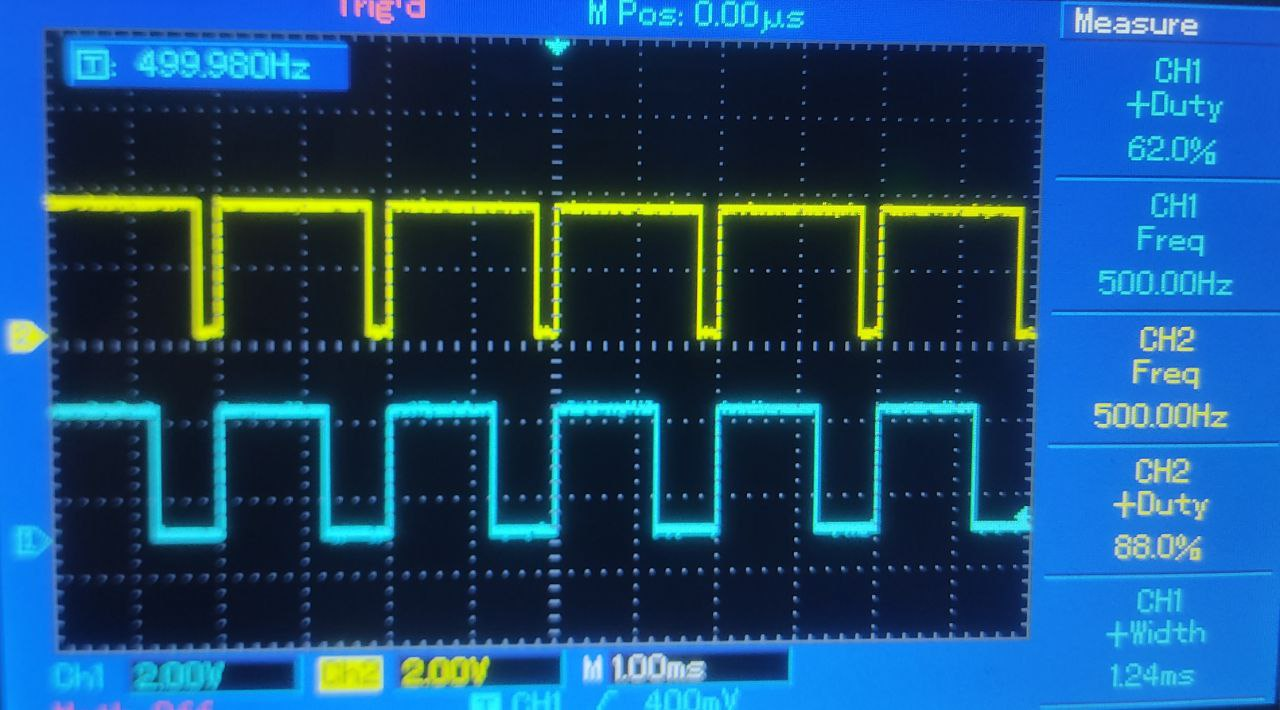
\includegraphics[width = \linewidth]{figures/PWMboth.jpg}
			\caption{Both Outputs}
			\label{fig:4:OscTest:both}	
		\end{subfigure}
		\caption{Results of the PWM output displayed on an oscilloscope.}
		\label{fig:4:OscTest}
	\end{center}
\end{figure} 
\section{Throttle}
\begin{figure}
	\begin{center}
		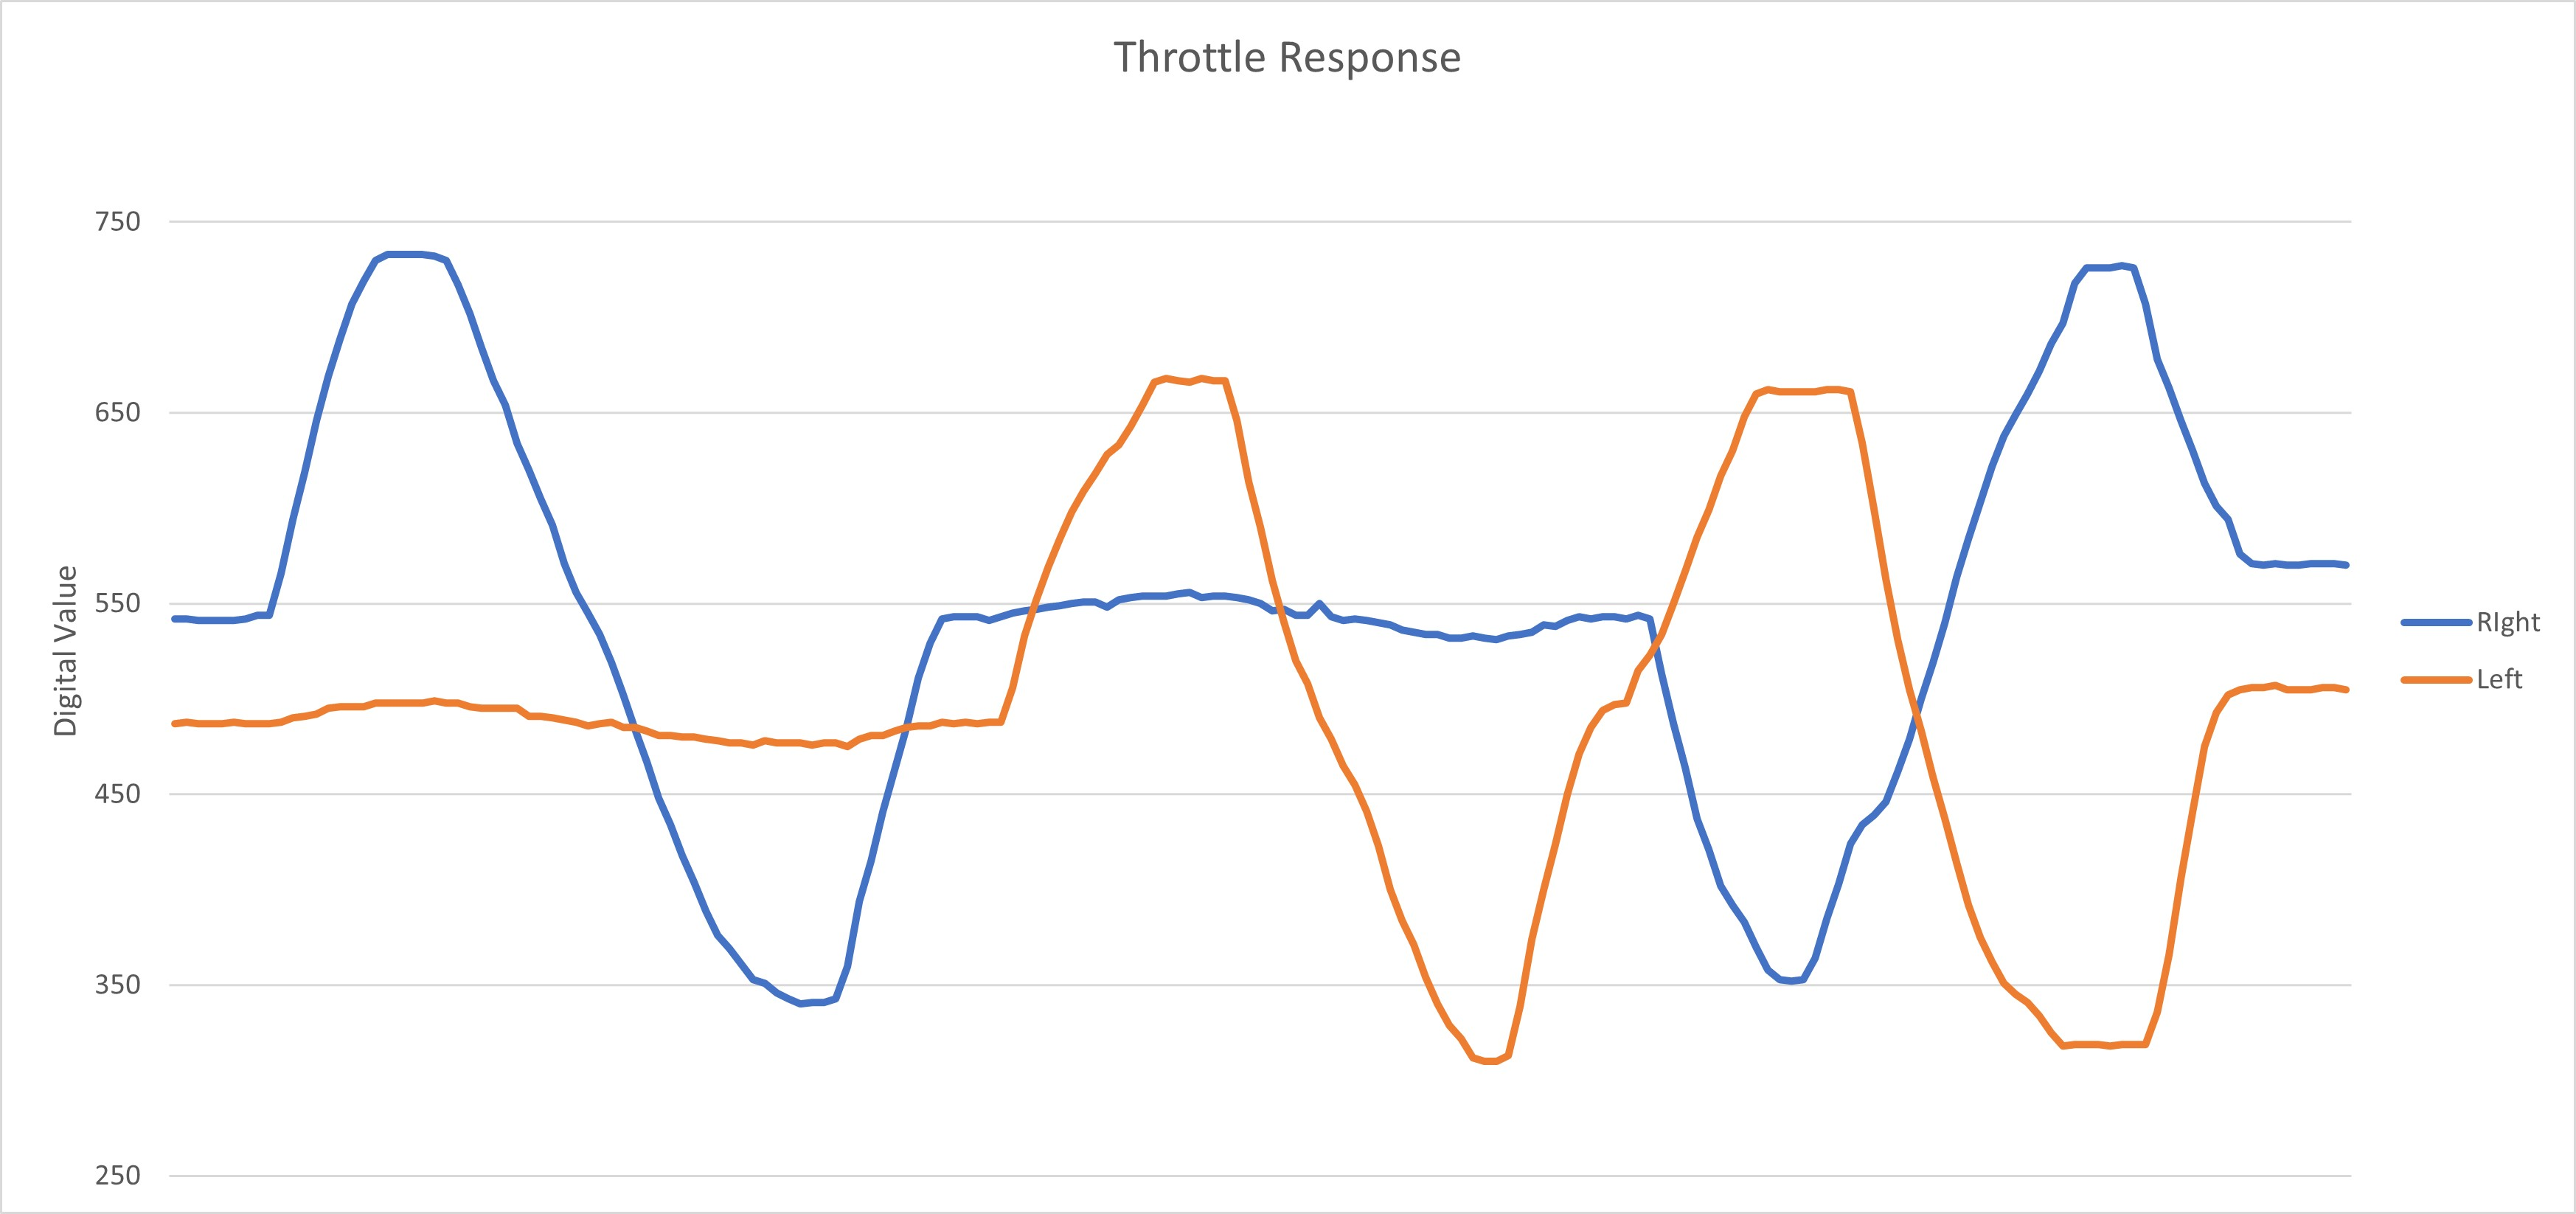
\includegraphics[width = 0.8\linewidth]{figures/graphThrottle.jpg}
		\caption{The digital response of the throttle.}
		\label{fig:4:Throttleresponse}
	\end{center}
\end{figure}
In order to test the response of the throttle and to show that the linear potentiometers have good accuracy the graph in \ref{fig:4:Throttleresponse} was plotted. It can clearly be seen that the potentiometers are meeting the upper and lower thresholds listed in \ref{tab:3:POT} and can move independently of each other without interference. Figure \ref{fig:4:Throttleresponse} also shows that in the neutral position there is some variation caused by user input when moving the other throttle. As one pushes on the one throttle one, will slightly pull on the other without realizing. Furthermore, even if it looks like the throttle is back in the neutral position, even a small amount off from the original position results in a different value. This is why the neutral buffer in \ref{tab:3:POT} was applied and it can be seen that buffer covers the slight variations. 
\begin{figure}
	\begin{center}
		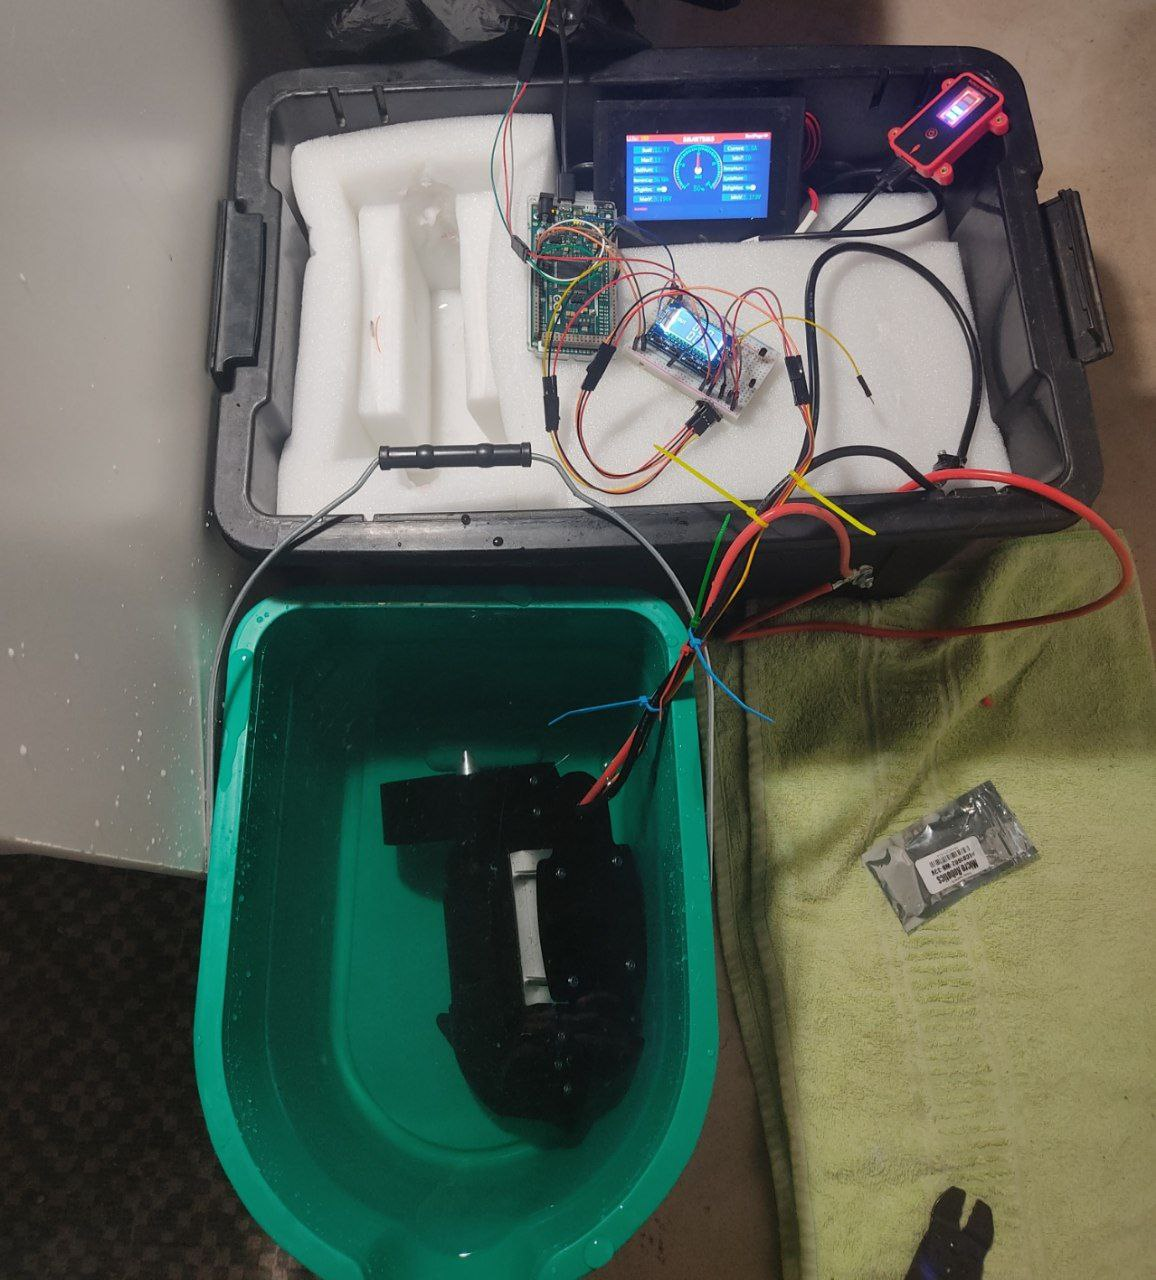
\includegraphics[width = 0.45\linewidth]{figures/thrusterBucket.jpg}
		\caption{The thruster in a bucket of water to test it without 'dry running'.}
		\label{fig:4:ThrusterTest}
	\end{center}
\end{figure}
\section{Thrusters}
The thrusters are designed to be operated in water as the water flow across the ESC is designed to dissipate the heat generated and prevent the ESC from overheating. Furthermore, the thruster is designed to push water and not air which have very different densities, so for these reasons the thrusters should not be 'dry run', and should only be operated while submerged. Figure \ref{fig:4:ThrusterTest} shows how, during the design and testing of the thrusters, a temporary water source was provide with a large bucket wherein the thrusters could be submerged to ensure that the thruster is responding to the PWM signal and giving the desired results.

\section{USV}
The final testing was conducted on the entire system as a whole by launching the vessel and operating it as a complete system. This section will first detail the procedure for setting up the system for a test followed by the details of how each test was carried out. Finally, the results of the full system tests will be discussed. 
\subsection{Set-up Procedure} 
The full system tests were carried out on the Stellenbosch canoe dam as it is a large enough body of water to sufficiently test the vessel and it is just outside of Stellenbosch so it is easily accessible. The system is transported completely disassembled so as to avoid any possible damages that could occur during transport. Therefore, before testing the vessel as well as the rest of the components must be set-up and checked before the vessel can be launched and the test can begin. Firstly the vessel and all safety equipment must be checked and prepared by following the checklist in table \ref{tab:4:boatCheck}. Once the vessel has be prepared the system can be assembled by following the checklist in table \ref{tab:4:equipCheck}. Once both of these checklists have been followed a final cursory sweep should be conducted to ensure that nothing has been missed and the vessel can be launched. Once the vessel is off of the trailer and in the water, the thrusters can be dropped down into their operational position. This will conclude the set-up of the vessel and the test can begin. 
\begin{table}
	\begin{center}
		
		\caption{Procedure to set-up the vessel and safety equipment}
		\label{tab:4:boatCheck}
		\begin{tabular}{|l|l|}
			\hline
			To Check: & Checked \\
			\hline
			All bungs are in place and secured. &\\
			\hline
			All tie downs are removed and stowed. &\\
			\hline
			The personal floatation device is aboard. &\\
			\hline
			The electrical fire extinguisher is aboard. &\\
			\hline
			There is no physical damage to the vessel that could cause leaks.&\\
			\hline
		\end{tabular}
	\end{center}
\end{table}
 \begin{table}
 	\begin{center}
 		\caption{Procedure to set-up the equipment and control system}
 		\label{tab:4:equipCheck}
 		\begin{tabular}{|p{0.65\linewidth}|l|}
			\hline
 			To Check: & Checked \\
 			\hline
 			Mount the throttle plate and secure the attaching bolts.&\\
 			\hline
 			Mount the control system under the throttle plate and secure the GPS and Compass onto the nose.&\\
 			\hline
 			Ensure that the thrusters are in the upright position and mount them onto the transom.&\\
 			\hline
 			Place the batteries at the back of the vessel, just in front of the transom.&\\
 			\hline
 			Ensure that the cut-off switch is in the off position and connect the thrusters to the batteries.&\\
 			\hline
 			Connect the control system to the thrusters. &\\
 			\hline
 			Check all connections to see that they are secure and that there are no open wires. &\\
 			\hline
 			Close the battery box and secure the battery box. &\\
 			\hline
 			Turn on the cut-off switch to power the system and check that the control system powers on. The thrusters should beep twice signifying that they are connected and receiving a signal.&\\
 			\hline
 			Wait until the GPS indicator light is on, signifying that the GPS has an valid GPS fix. &\\
 			\hline
 		\end{tabular}
 	\end{center}
 \end{table}
\subsection{Testing}
The testing occurred in two phases, the manual test and the autonomous test. The manual test was carried out by using the throttle to manually control the vessel and ensure that the thrusters are responding correctly and that the system is fully operational. The GPS points that the boat would navigate to under autonomous control were chosen while doing the manual test to ensure that the vessel would not navigate into any of the obstacles on the dam such as buoys and pumps.\par
Finally, for the autonomous test, the vessel was driven back to the starting position and the system was reset and autonomous navigation was selected. The vessel was still manned so that manual control could be taken at any point if it looked as though the vessel would collide with any obstacles. Once the vessel had navigated to its final point, manual control was selected to return the vessel to shore. 
\begin{figure}[!hb]
	\begin{center}
		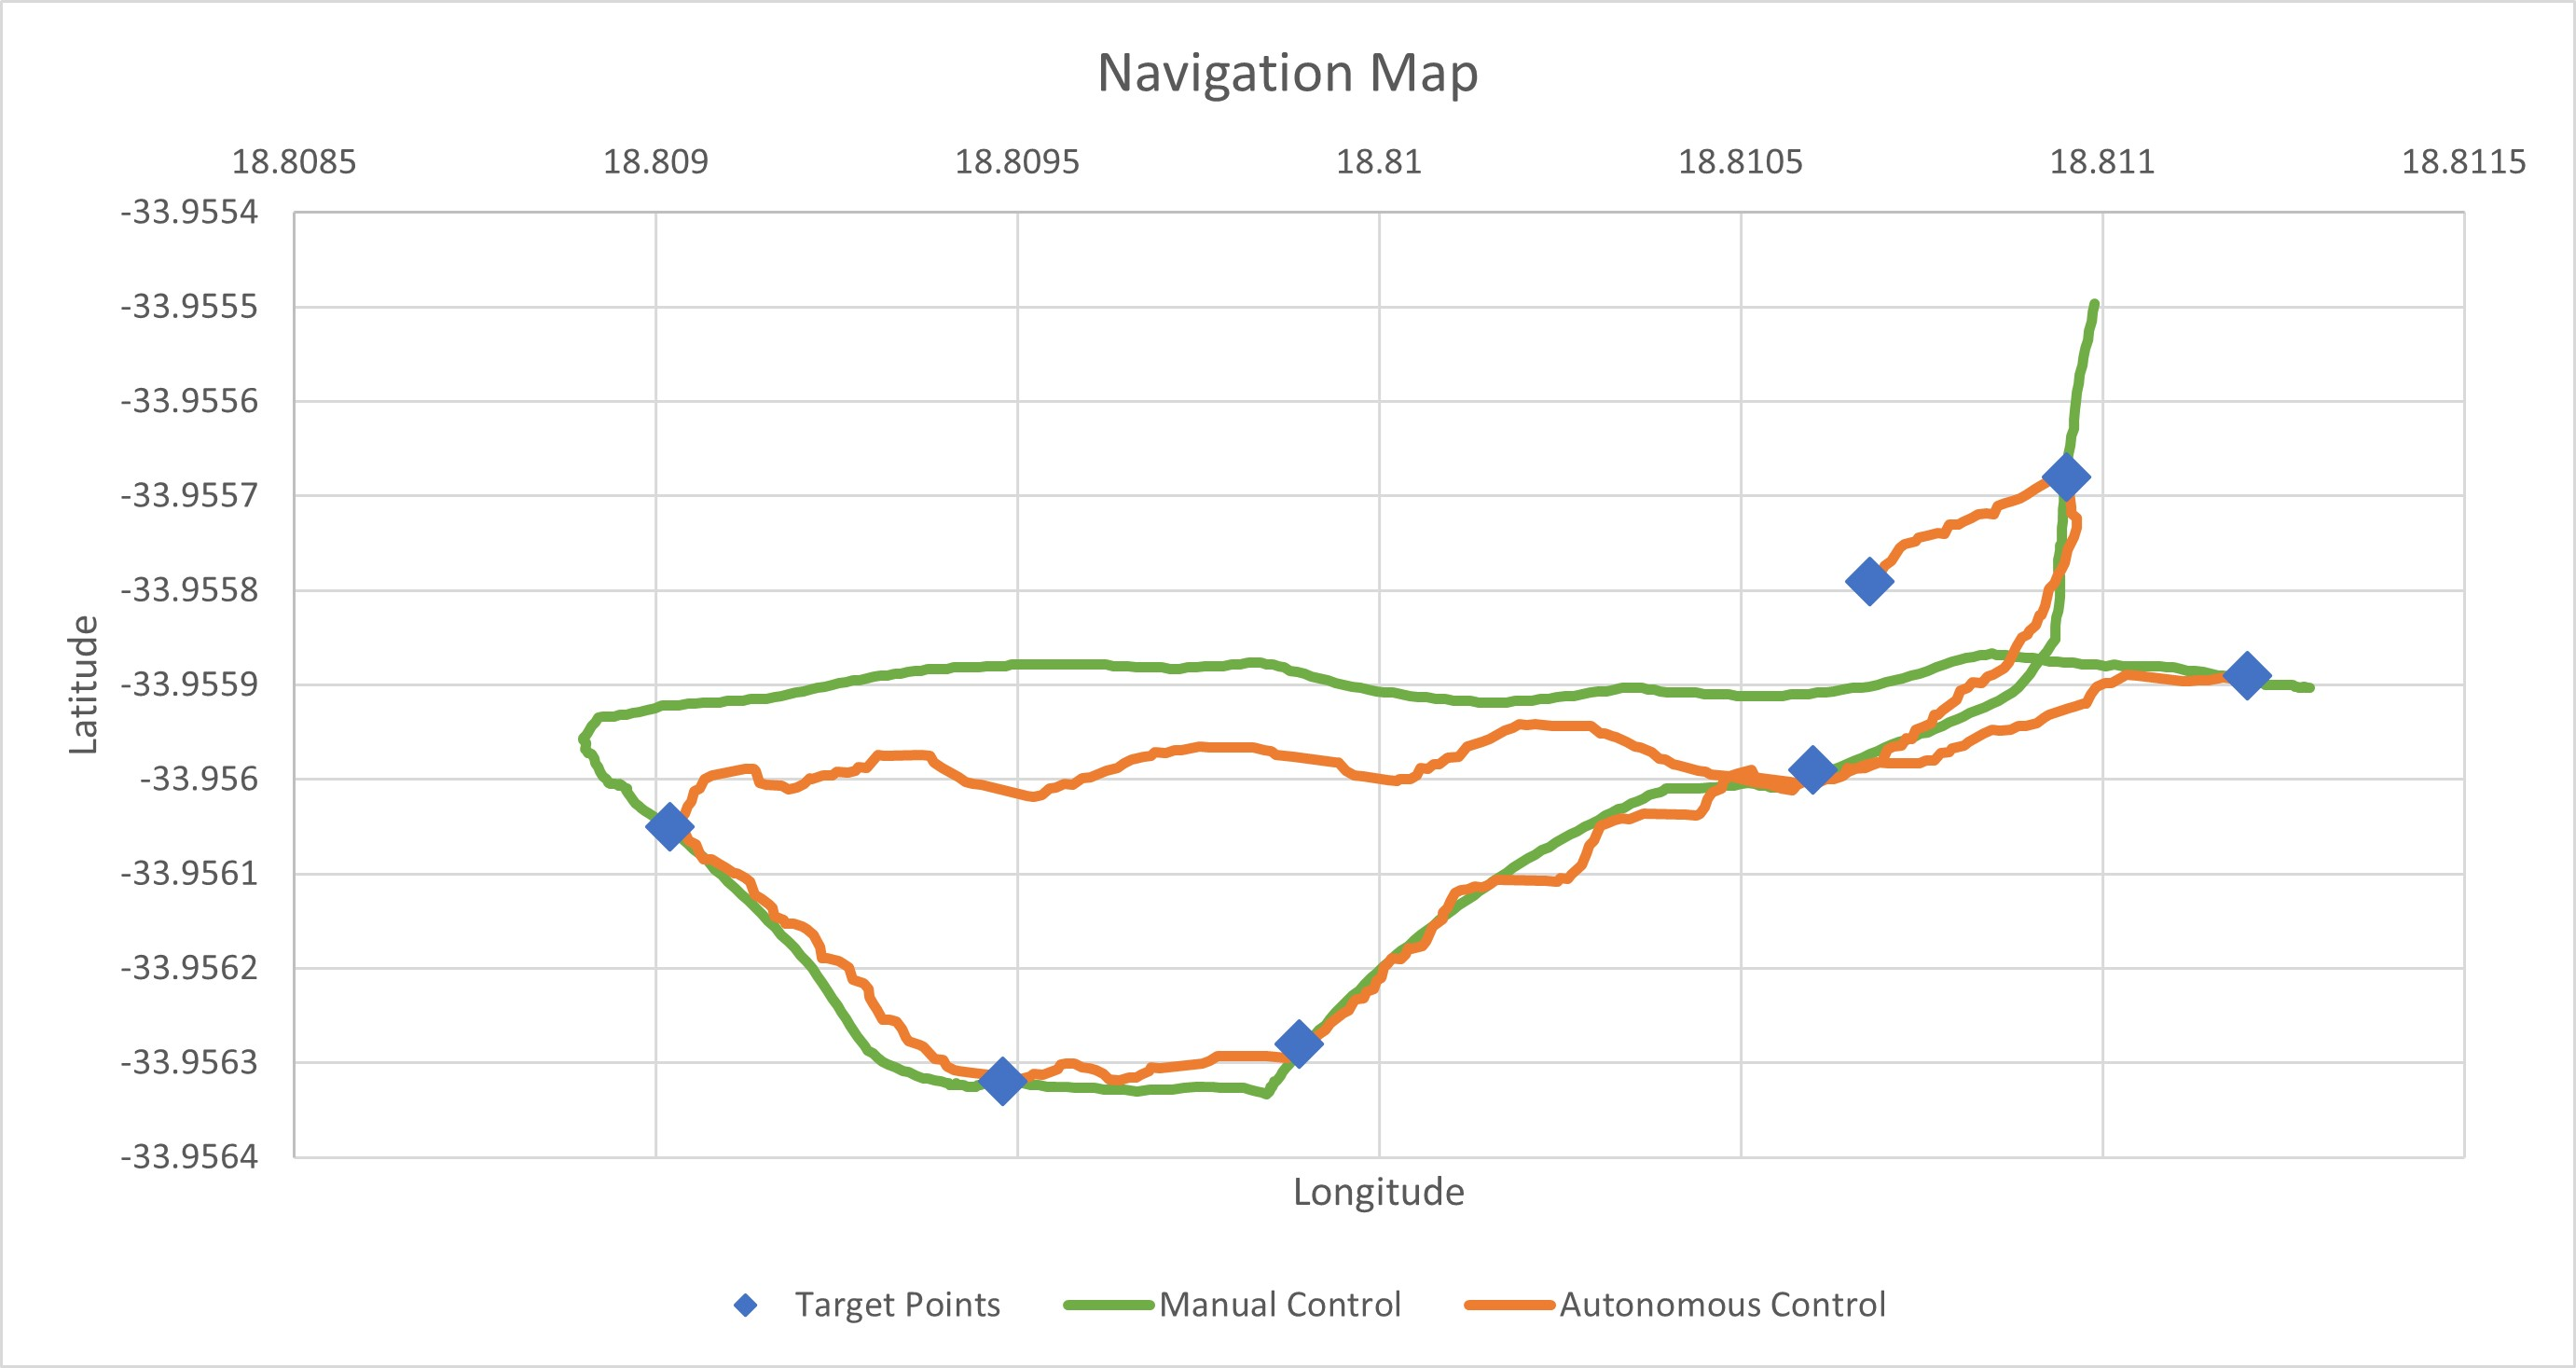
\includegraphics[width = 0.84\linewidth]{figures/graphMap.jpg}
		\caption{Map of Test 1.}
		\label{graph:4:Map}
	\end{center}
\end{figure}
\vspace{0.8cm}
\subsection{Results}
After all the testing had been completed, the results could be analysed and assessed to determine the validity and performance of the control system. The results will be discussed with the aid of graphs draw from the data collected during the tests. The performance of the control system will be determined by how accurately it stays on the course to the target location and the validity of the system will be determined by if the vessel reached the target points. \par
The initial autonomous test carried out was successful in that it navigated to the points after some time. However, there was a lot lacking as the navigation was very far off course for large portions of the test. Figure \ref{graph:4:Map} shows the route of the manual test and the first autonomous test, the manual test is also shown in Figure \ref{graph:4:Map2} as a reference point between the two autonomous tests. It can be seen in Figure \ref{graph:4:Map} that the vessel does navigate to the points but there are large unnecessary loops that the vessel travels. This points to the navigation system being valid but very inaccurate. Once the data could be analysed, it became apparent that the inaccuracy was caused by the compass having lost calibration. The data showed that even on the long looping path, the compass reading was within \SI{40}{\degree} of the target bearing which was clearly incorrect. It appears that the compass had accurate calibration in the approximate range of \SI{350}{\degree} to \SI{150}{\degree}. This is further backed up by how the vessel always followed a long loop until the point was within this range, at which point it would successfully navigate to the point. Due to the inaccuracy of the test and the underlying cause being a faulty sensor and not a flaw in the system, another test was planned.\par
\vspace{0.6cm}
The second autonomous test was conducted under less than ideal conditions with a steady wind blowing from the South East. However, even under these conditions the system performed well and navigated to within the acceptable distance of \SI{7}{\metre} of each point. Figure \ref{grph:4:distance} shows the distance to the targeted point as the time elapsed. It can clearly be seen that the vessel was a path of steadily decreasing the distance to the point until arrival. The only exception is just before arriving at point 5, the distance slightly increases. This was due to the vessel heading straight at a buoy. The vessel was pushed off against the buoy to avoid contact the system handled the disruption by correcting its course and navigating back to the target.\par 
The disruption can further be seen in Figure \ref{grph:4:BearingError} with a large spike in the difference between the vessel bearing and the target bearing. This spike is corrected and the course is resumed. The other large spikes on Figure \ref{grph:4:BearingError} all correlate with the arrival at a point upon which the target is moved to the next point and a large error occurs before the system can turn itself and navigate to the next point. Another trend of Figure \ref{grph:4:BearingError} shows that the vessel settles around \SI{10}{\degree} off from the target bearing. This is not a large static error and could be tuned out in the control system, however more tests would need to be conducted to ensure that the static error is not caused by external factors such as the steady wind during the test. \par
The steady error can also be seen in Figure \ref{grph:4:2bearings} where the vessels bearing is mostly just above the target bearing. However, Figure \ref{grph:4:2bearings} also clearly shows that the vessel reacts well to changes in the target bearing and tracks the target bearing closely with minimal overshoot. The sudden change of bearing between points 4 and 5 in Figure \ref{grph:4:2bearings} is due to the vessel turning across the \SI{360}{\degree}-\SI{0}{\degree} turnover point. \par
Another trend that can be seen across both Figures \ref{grph:4:BearingError} and \ref{grph:4:2bearings} is that the vessel has a large amount of oscillation and is often referred to as 'fish tailing'. The oscillations can be explained by the thrusters that were used. Even with the increase in voltage the thrusters were underpowered in comparison to the weight and shape of the vessel. This meant that the steering was slow to respond and the progressive steering implemented was not very noticeable. To further compound on the issue, it became apparent during the manual test that one thruster produced slightly more thrust than the other leading to a slight drift when both thruster were fully powered and also allowed the vessel to be more manoeuvrable when turning one direction as opposed to the other. However, given these oscillations when looking at the overall navigation map of Figure \ref{graph:4:Map2} the path of the vessel is relatively straight in the overall distance travelled. Figure \ref{graph:4:Map2} shows the effect the wind had with a small effect evident on the route between points 2,3 and 4 with the vessel into the wind. However, between points 5 and 6, when the vessel was travelling mostly with the wind, it had a large impact and blew the vessel off course and the system had to correct to finally reach point 6.\par
Overall the system performed well with less than ideal weather conditions and underpowered and slightly uneven thrusters. Given these, the system still managed to navigate to within the prescribed allowable distance and maintain a relatively straight route between all points and not doing any unnecessary navigation. The system could easily be upgraded to a larger more appropriate vessel with the required thrust with little alterations.

\begin{figure}
	\begin{center}
		\begin{subfigure}{0.8\linewidth}
			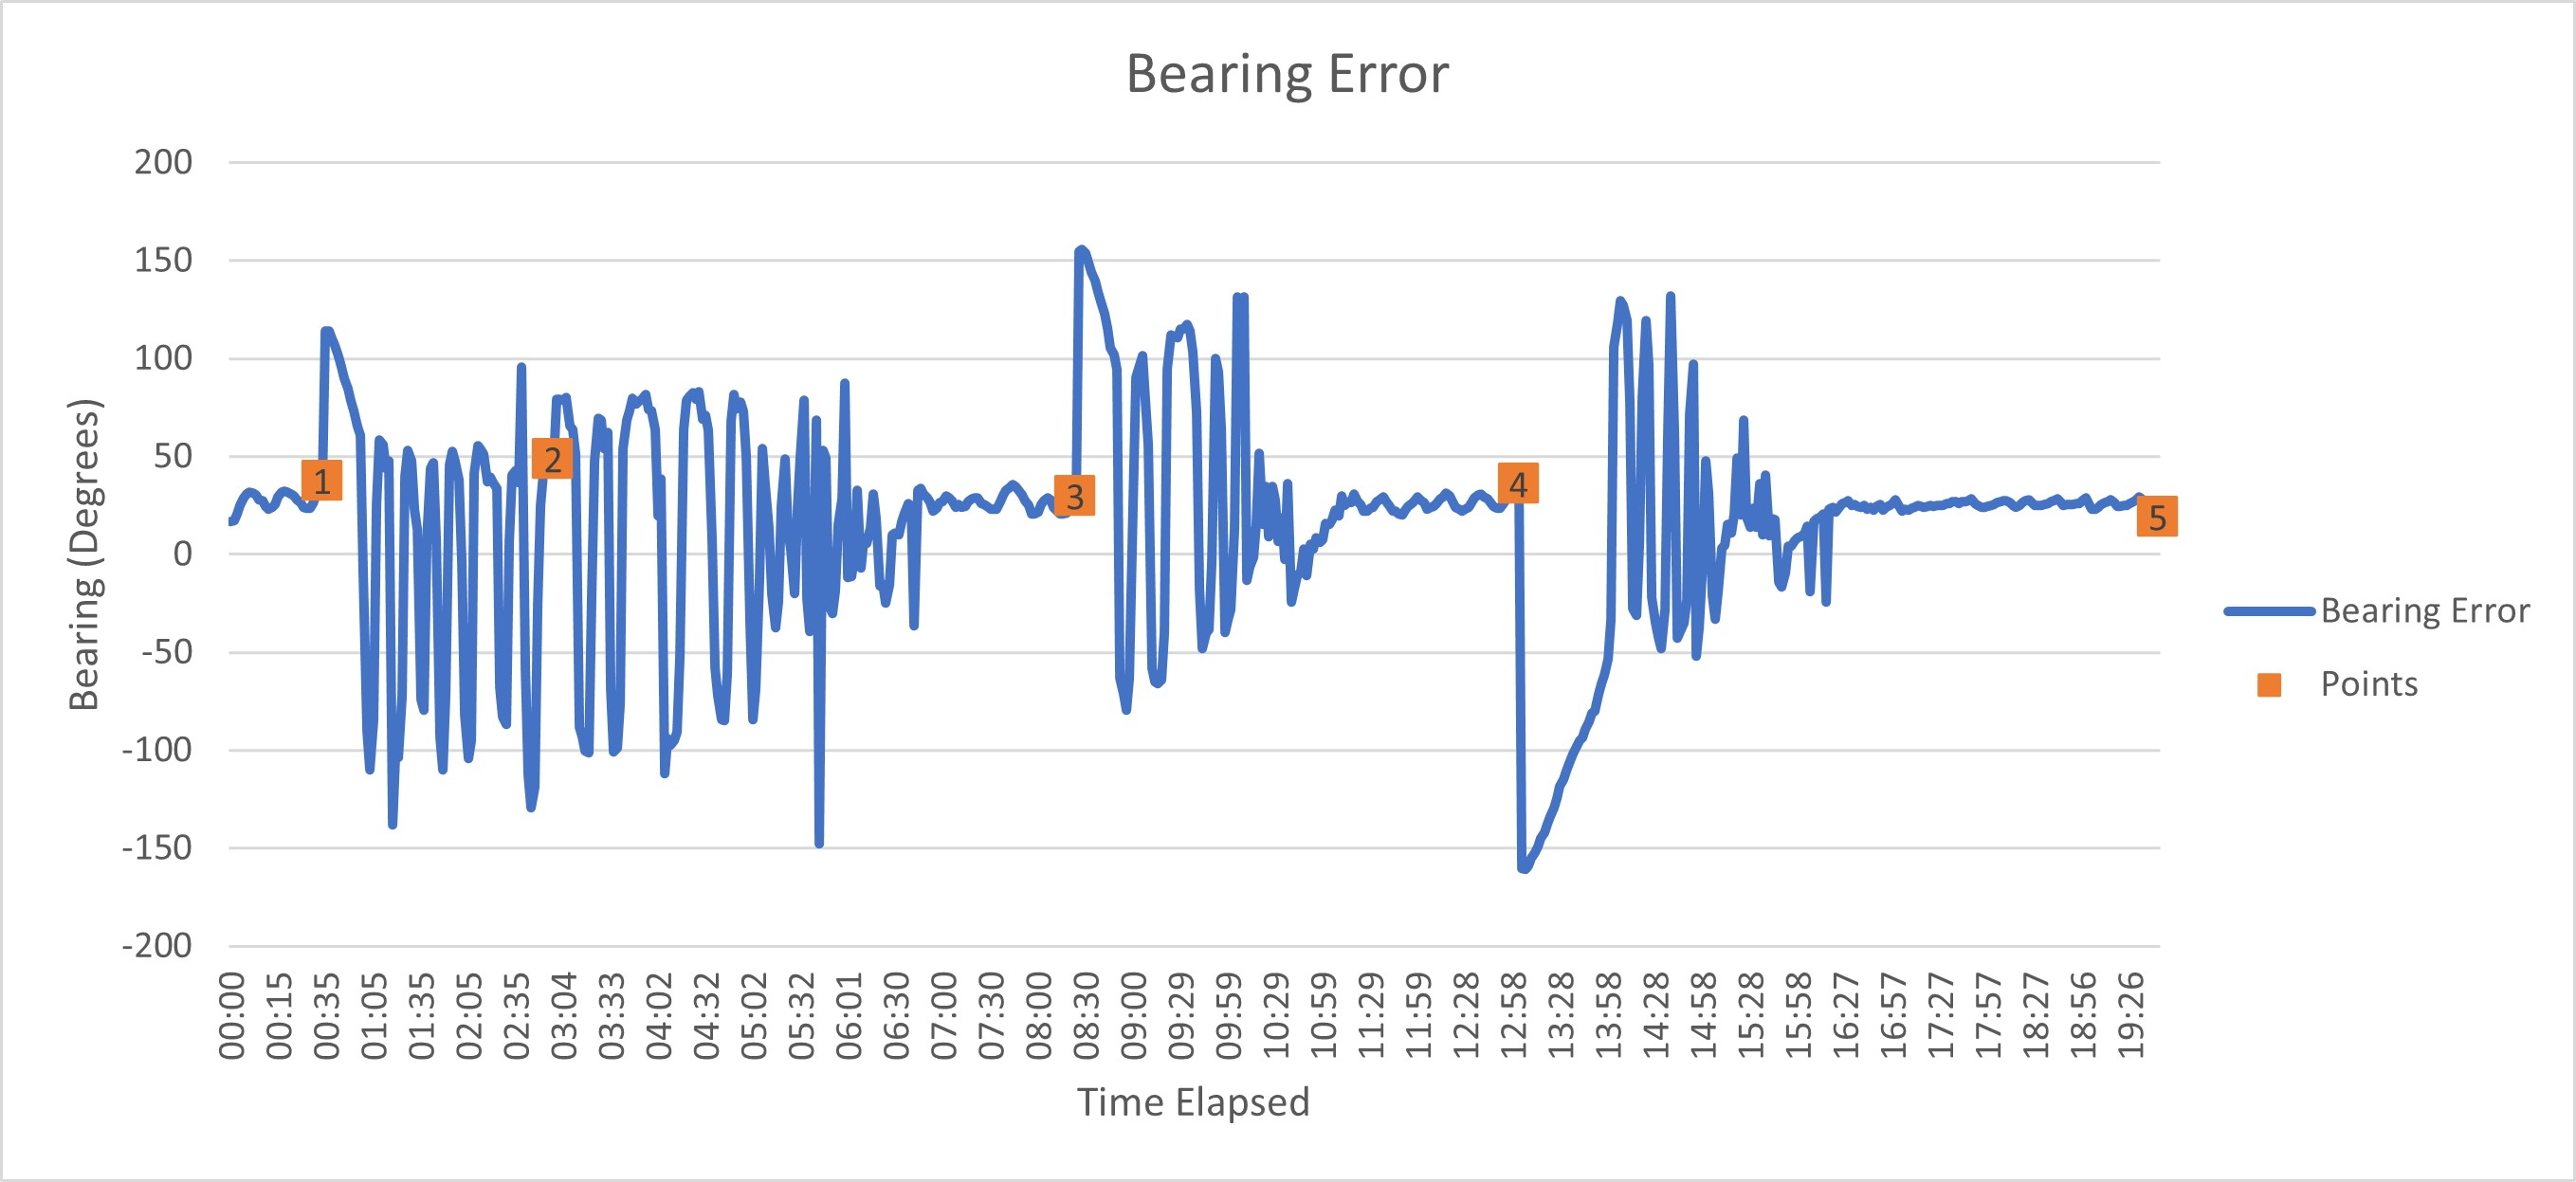
\includegraphics[width = \linewidth]{figures/graphBearingError.jpg}
			\caption{Bearing Error.}
			\label{grph:4:BearingError}	
		\end{subfigure}
		\begin{subfigure}{0.8\linewidth}
			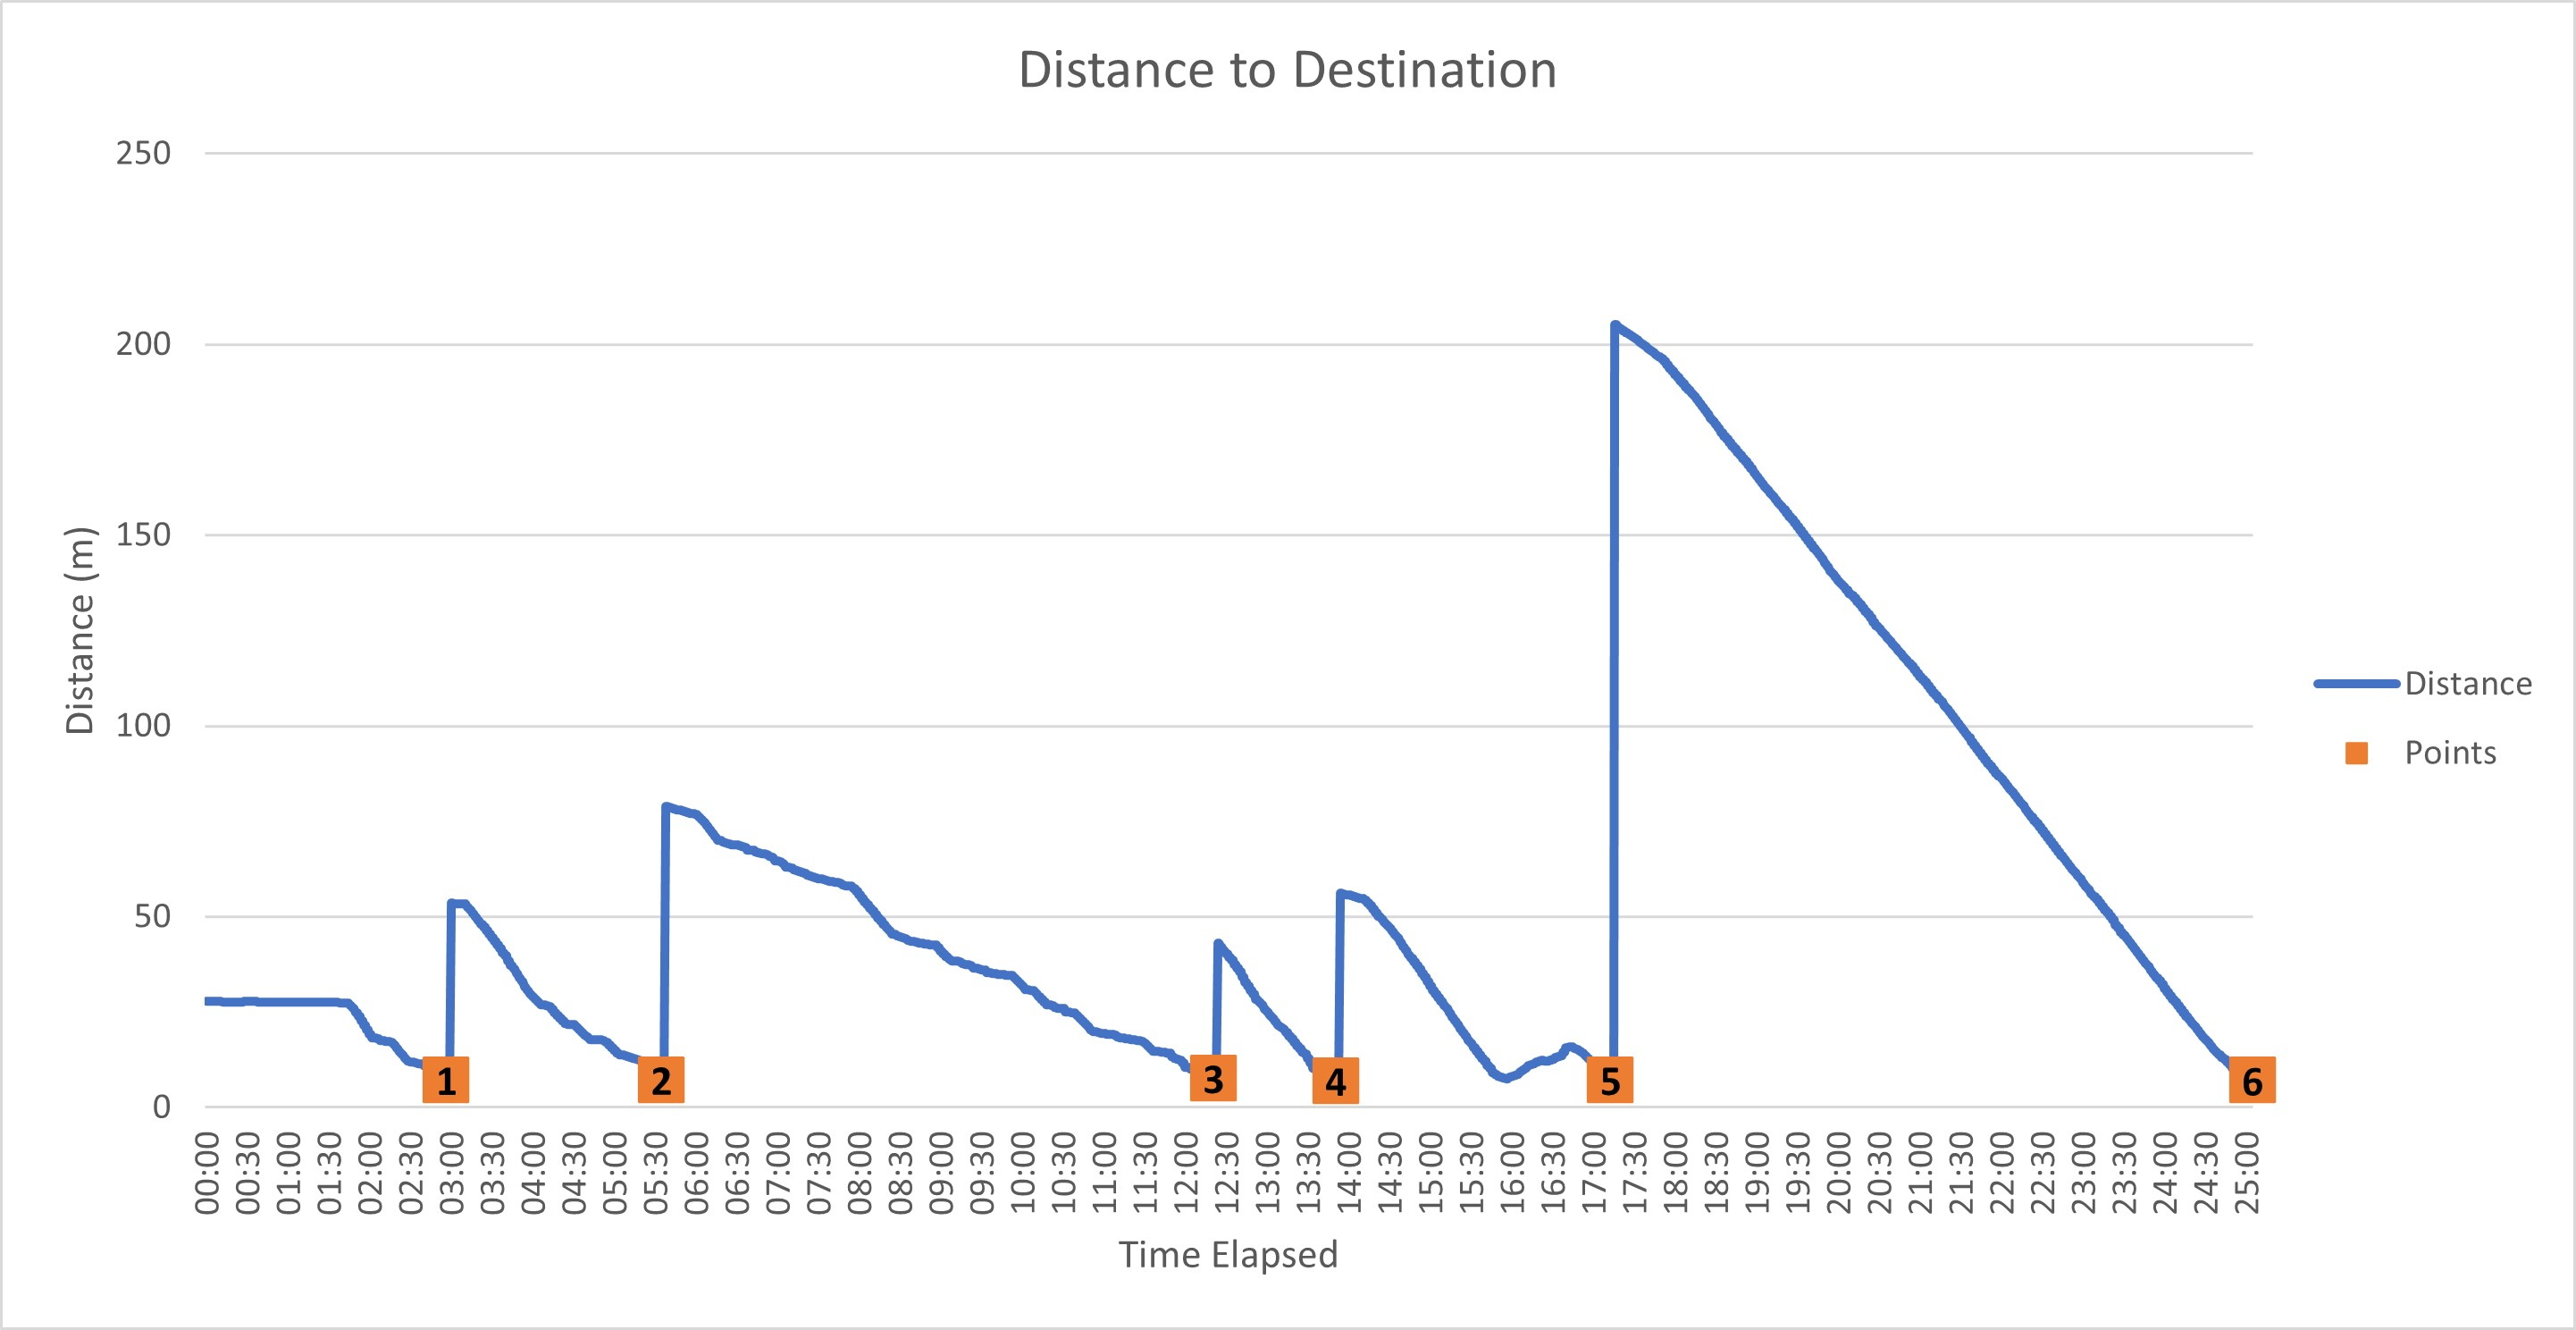
\includegraphics[width = \linewidth]{figures/graphDistance.jpg}
			\caption{Distance to Target.}
			\label{grph:4:distance}	
		\end{subfigure}
		\begin{subfigure}{0.8\linewidth}
			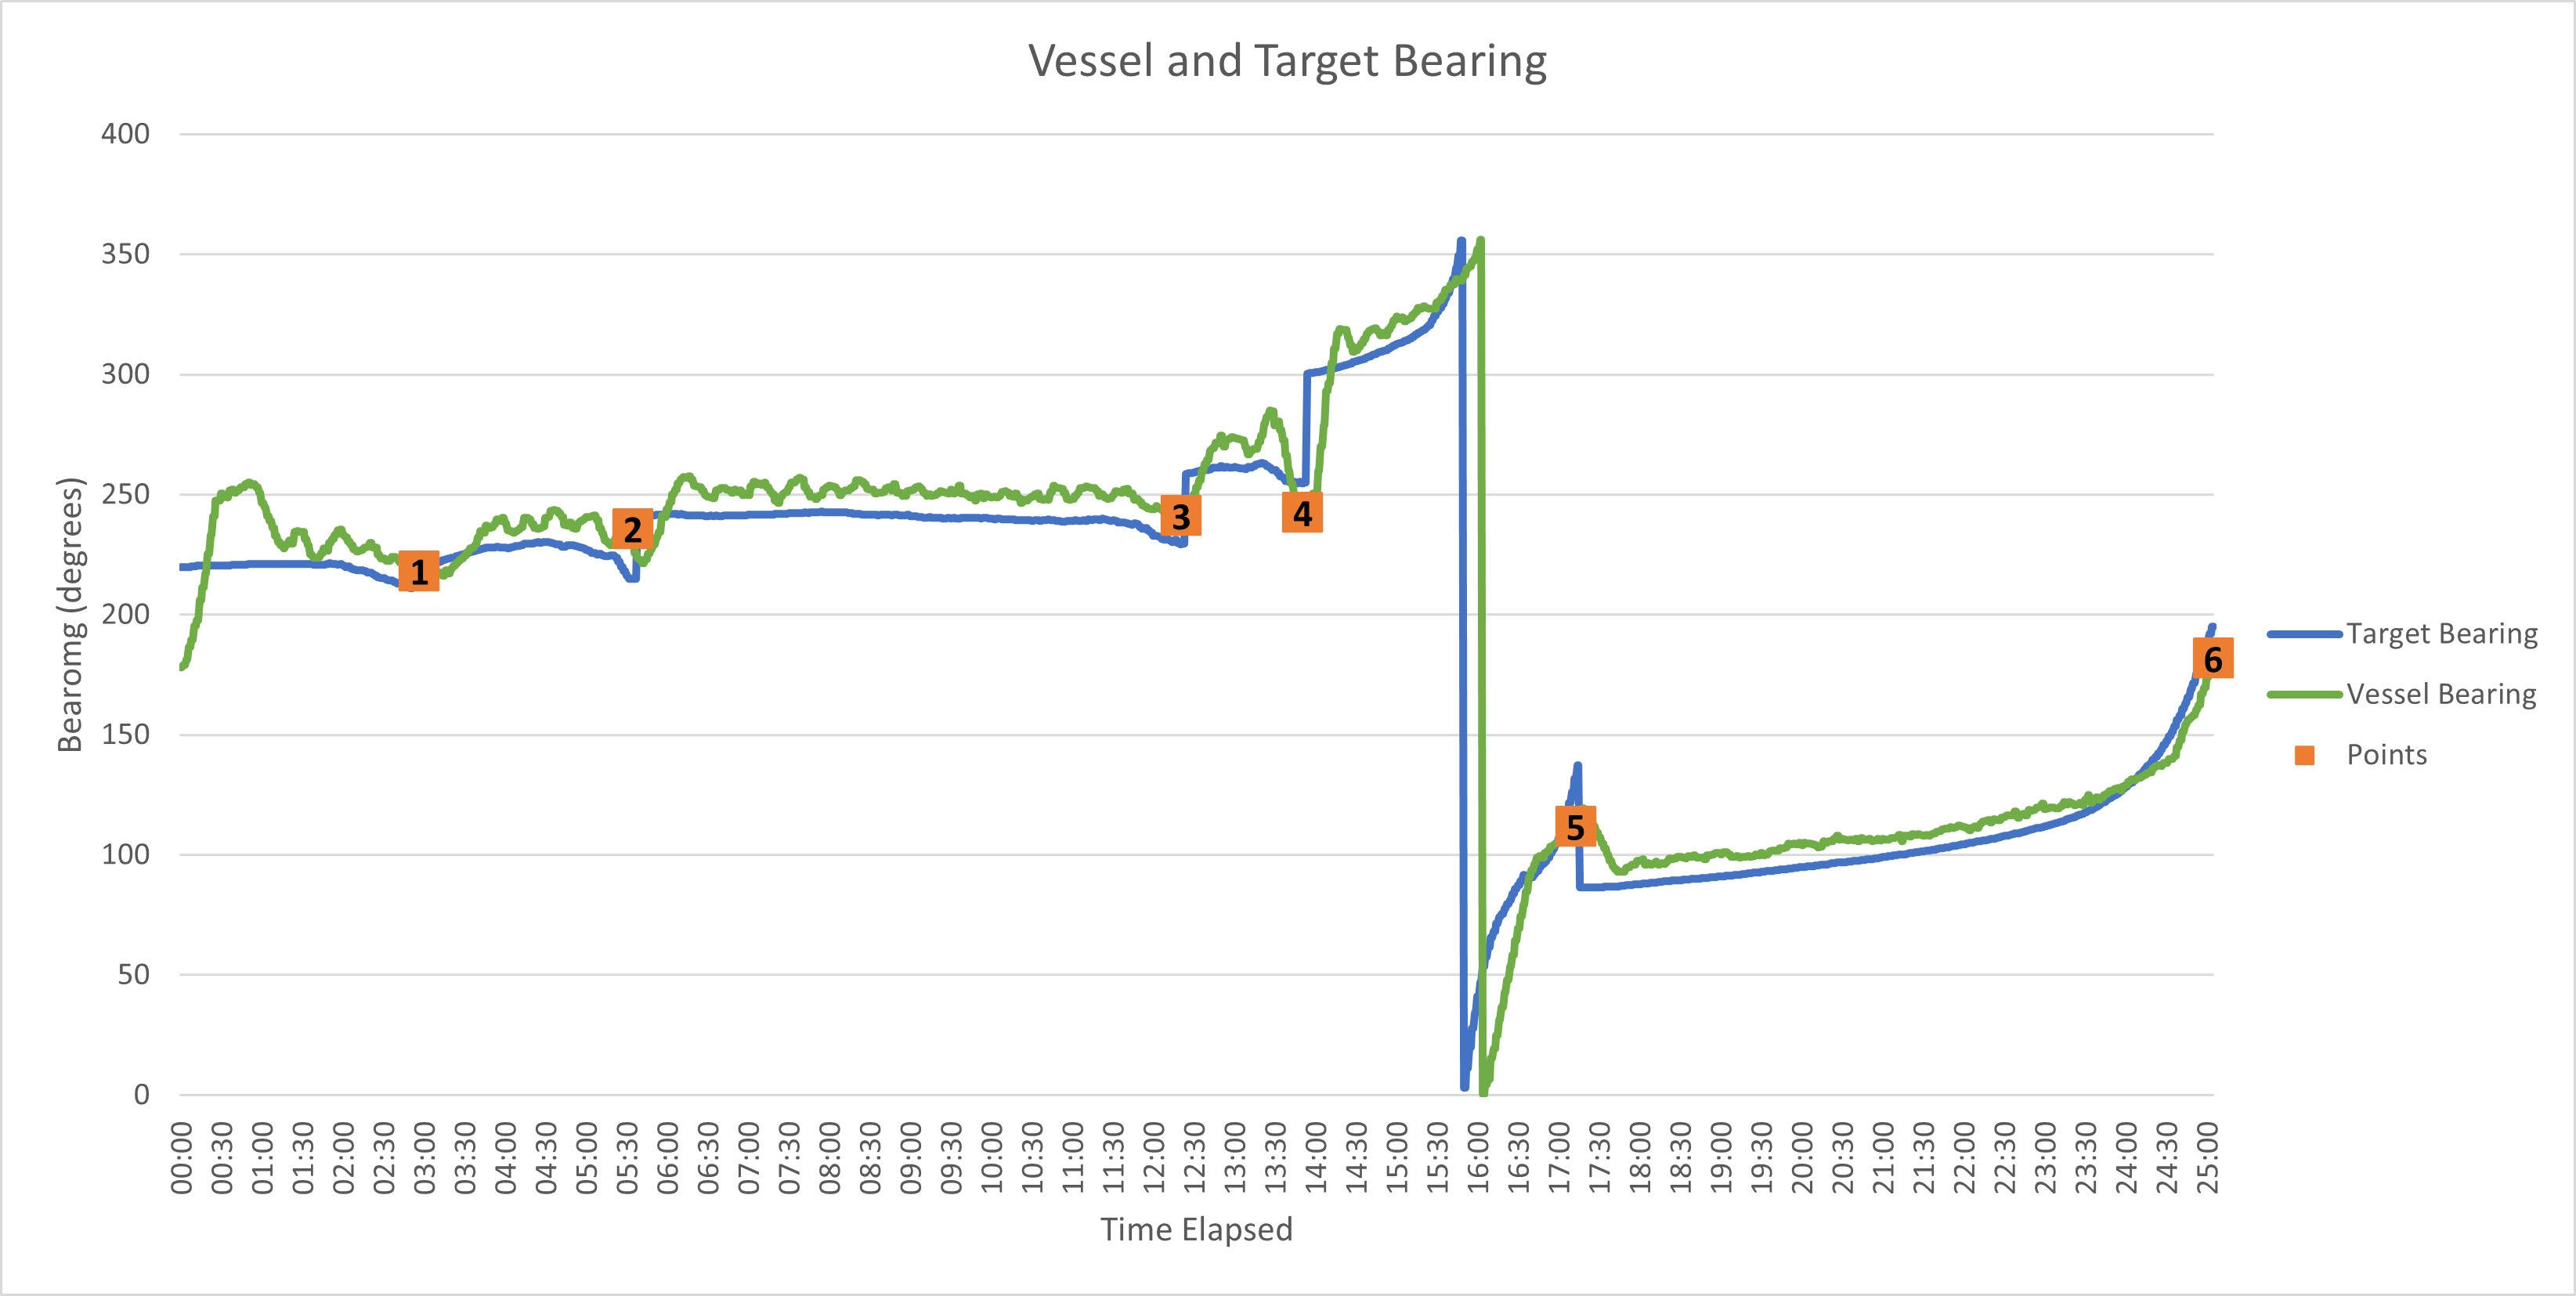
\includegraphics[width = \linewidth]{figures/graphBearings.jpg}
			\caption{Bearings Comparison.}
			\label{grph:4:2bearings}	
		\end{subfigure}
		\caption{Results of the PWM output displayed on an oscilloscope.}
		\label{fig:4:Results}
	\end{center}
\end{figure} 
\begin{figure}[hb]
	\begin{center}
		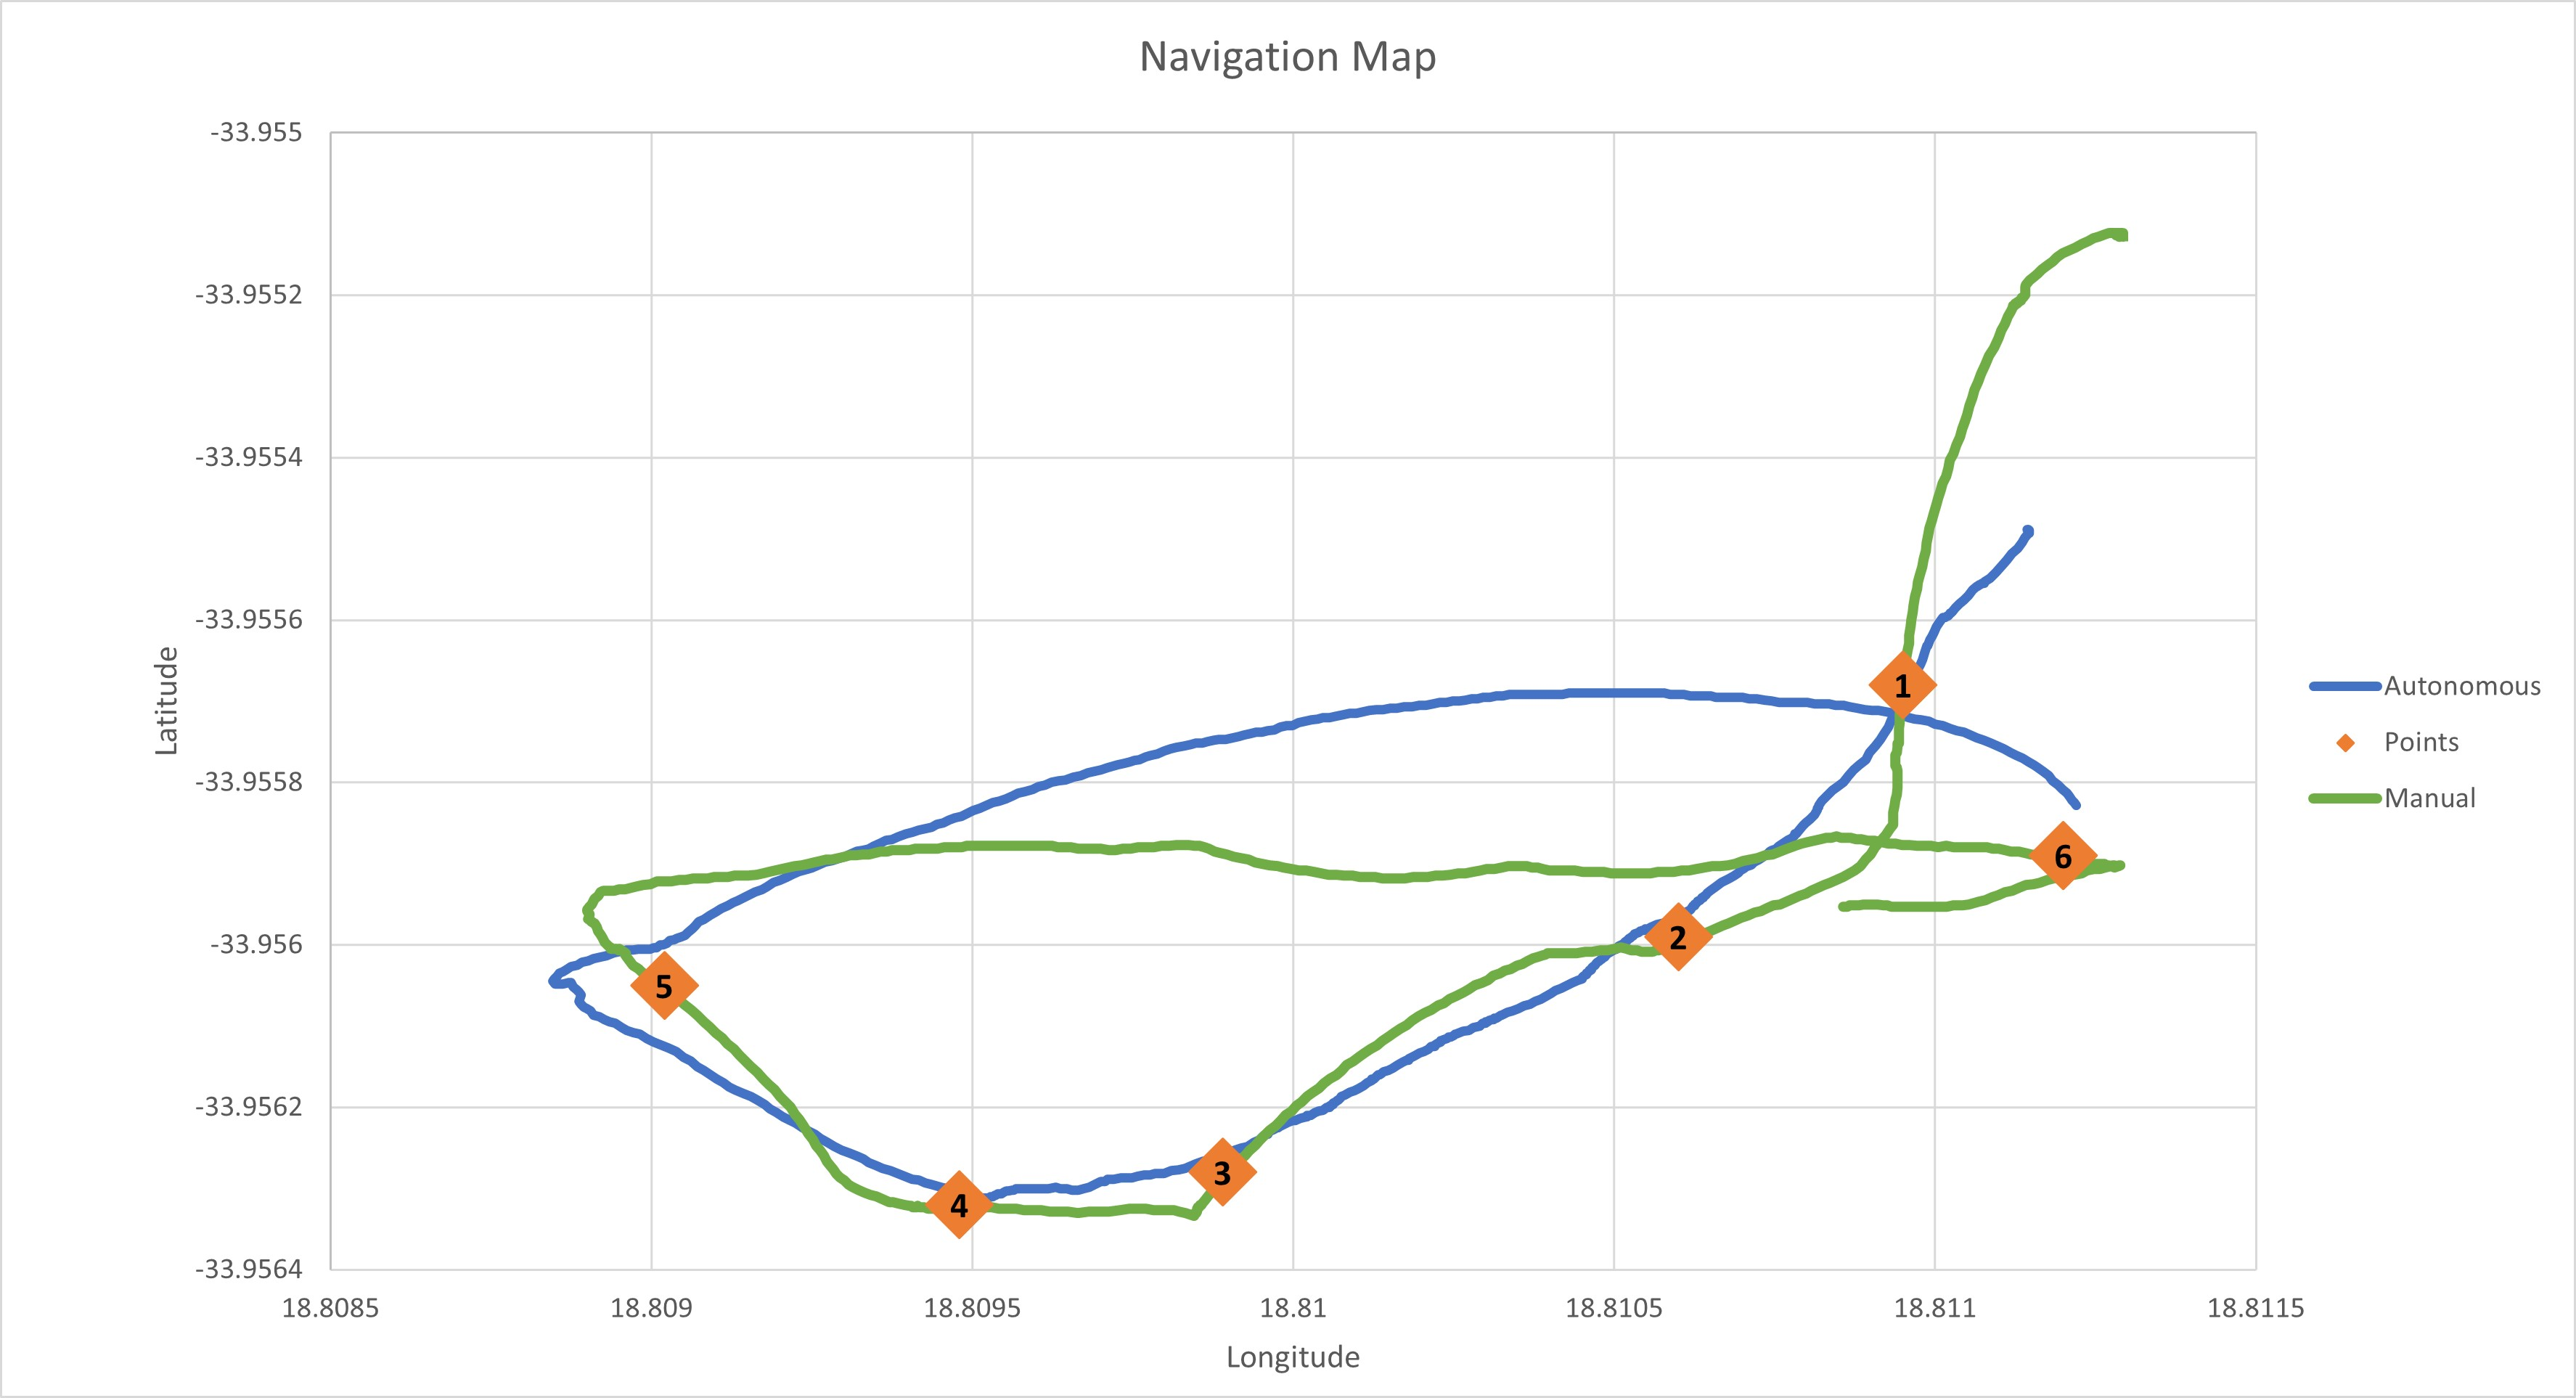
\includegraphics[height=0.8\linewidth, angle = 270]{figures/graphMap2.jpg}
		\caption{Map of Test 2.}
		\label{graph:4:Map2}
	\end{center}
\end{figure} 
\chapter{Conclusion}
The objective of this project was to design and construct a prototype control system for an unmanned surface vessel. It would need to have a manual control option for testing in addition to the autonomous navigation system.
\section{Achieved}
The individual system test went well and no major issues were found. Although, the thrusters were slightly underpowered this was not a technical issue. The first autonomous test showed that the system could navigate to the points but due to the compass loosing calibration this was not accurate navigation. Finally, in the second autonomous test the system navigated accurately between the points and reached each target point. There was also a steady wind that blew the vessel off course and the system was able to counter this and still reach its target destination. The control system achieved its goal and would be able to be implemented into a larger system with minimal alterations. 
\section{Future Development}
A fully autonomous unmanned surface vessel would require more development in order for it to be safe and sustainable on the ocean. A primary requirement would be to add obstacle avoidance both above and below water so that the vessel could navigate debris, other vessels and shallow waters. This would also tie into a 'return home' feature that would allow the vessel to return to its starting point, avoiding any obstacles, if it encountered any problems or once it had completed its course. \par
It was mentioned that the thrusters in this project were underpowered and so it would be worthwhile investigating more powerful and efficient thrusters. However, more powerful thrusters would require a larger power supply. Future development can investigate renewable power regeneration such as solar to recharge the power supply and extend the range of the system. Furthermore, sensors to detect wind and current flow together with weather mapping could be used to plot the most efficient route the vessel can take working with the elements instead of against them. 

\bibliography{bib}

\appendix%===========================================================


\chapter{Techno-Economic Analysis}
This appendix contains details on the cost of the project both in terms of materials and supplies as well as the cost of the Electrical Engineering workshop and the cost of a junior engineers time to complete the project. The second part of the appendix is a Gantt chart detailing the timeline of the project. The Gantt chart is broken down into five sections. The introductory stage includes the project proposal and initial literature review. There are two build stages, one for the control system and electronics and one for the boat and thruster mounts. The fourth stage is the testing and analysis of the system and the final stage is the writing up of the final report. \par
\newpage
\begin{landscape}
	\small
\section{Budget}
\begin{tabular}{|p{0.2\linewidth}|p{0.03\linewidth}|p{0.06\linewidth}|p{0.08\linewidth}|p{0.08\linewidth}|p{0.08\linewidth}|p{0.03\linewidth}|p{0.06\linewidth}|p{0.08\linewidth}|p{0.08\linewidth}|}
	\hline
	\textbf{Activity} & \multicolumn{2}{p{0.09\linewidth}|}{\textbf{Engineering Time}} & \textbf{Running Costs} & \textbf{Facility Use} & \textbf{Capital Costs} & \multicolumn{2}{p{0.09\linewidth}|}{\textbf{MMW}} & \textbf{MMW} & \textbf{Total} \\
	\hline
	&  &  &  &  &  & \multicolumn{2}{c|}{\textbf{Labour}} & \textbf{Material} &  \\
	\hline
	& \textbf{hr} & \textbf{R} & \textbf{R} & \textbf{R} & \textbf{R} & \textbf{hr} & \textbf{R} & \textbf{R} & \textbf{R} \\
	\hline
	Review Literature & 25 & 11250 & 150 &   &   &   &   &   & \textbf{11425} \\
	\hline
	Review Similar Projects & 20 & 9000 &   &   &   &   &   &   & \textbf{9020 }\\
	\hline
	Design the Algorithm Flow Diagram & 15 & 6750 &   &   &   &   &   &   & \textbf{6765 }\\
	\hline
	Design the Control System Hardware & 10 & 4500 &   &   &   &   &   &   & \textbf{4510}\\
	\hline
	Design the Mechanical Mountings & 10 & 4500 &   &   &   &   &   &   & \textbf{4510 }\\
	\hline
	Create Parts List & 5 & 2250 &   &   &   &   &   &   & \textbf{2255 }\\
	\hline
	Order Parts List & 5 & 2250 & 3000 &   & 45700 &   &   &   & \textbf{50955 }\\
	\hline
	Manufacture Mechanical Mountings & 20 & 9000 &   &   &   & 45 & 13500 & 1500 & \textbf{24065} \\
	\hline
	Manufacture the Control System Hardware & 25 & 11250 & 250 &   &   &   &   &   & \textbf{11525} \\
	\hline
	Program the Control System Algorithm & 35 & 15750 &   &   &   &   &   &   & \textbf{15785 }\\
	\hline
	Fix all System Elements & 20 & 9000 & 300 &   &   &   &   &   & \textbf{9320 }\\
	\hline
	Test USV in Manual Mode & 90 & 40500 & 1500 &   &   &   &   &   & \textbf{42090 }\\
	\hline
	Test USV in Self-navigating Control & 150 & 67500 & 1500 &   &   &   &   &   & \textbf{69150 }\\
	\hline
	Compile Final Report & 100 & 45000 &   &   &   &   &   &   & \textbf{45100 }\\
	\hline
	\textbf{Total} & \textbf{530} & \textbf{238500} & \textbf{6700} & \textbf{0} & \textbf{45700} & \textbf{45} & \textbf{13500} & \textbf{1500} & \textbf{306475} \\
	\hline
\end{tabular}

\normalsize
\section{Schedule}

	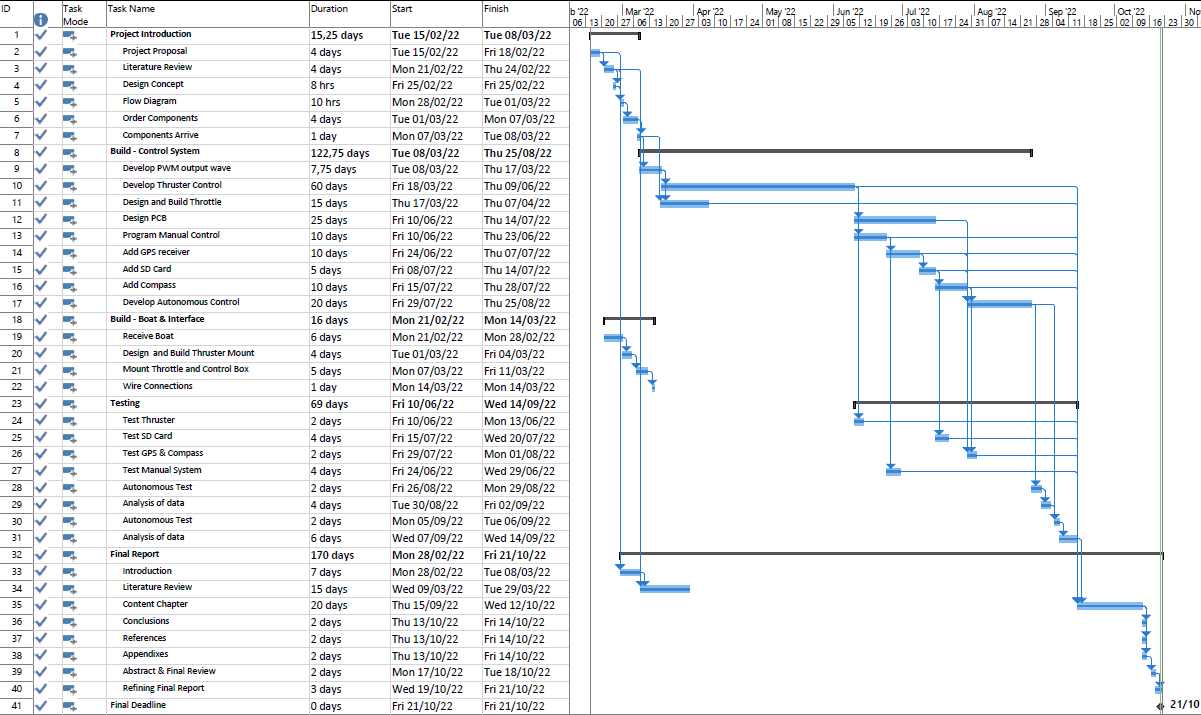
\includegraphics[width = \linewidth]{figures/Schedule.png}	


\end{landscape}
\chapter{Safety Procedures}
The Stellenbosch Engineering laboratories were not used in this project however, once the prototype was developed there were several tests with the system on a dam. There are risks involved in this testing. Table \ref{saf} is the activity based risk assessment that shows the risks associated with the project and the mitigation taken to limit the effects of these risks. Overall the mitigations worked as there was risk occurrence. An incorrect connection was made leading to a short circuit and damaging the one ESC. 

\begin{table}
	\caption{Activity Based Risk Assessment}
	\label{saf}
\begin{tabular}{|m{2.5cm}|m{2.5cm}|m{1cm}|m{3cm}|m{6cm}|}
	\cl{1-5}
	\textbf{Activity} & \textbf{Risk} & \textbf{Risk Type} & \textbf{Classification of risk severety} &\textbf{ Mitigating Steps} \\
	\cl{1-5}
	\multirow{2}{2cm}{Launching Vessel} & Vessel sinking & E & Acceptable Risk & Ensure that the bungs are securely sealed \\
	\cl{2-5}
	& Vessel floating away & E & Acceptable Risk & Ensure a secondary rope is attached to the vessel to pull it back once it is off the trailer \\
	\cl{1-5}
	Connecting Electronic Equipment & Short Circuit & E & Substantial Risk & Double check which connection is the correct one before connecting them. \\
	\cl{1-5}
	Connecting Battery System & Electrical Shock & P & Possible Risk & Ensure the power switch is off before connecting the terminals and connect one terminal at a time and next touch both terminals. \\
	\cl{1-5}
	Operating Vessel & Cut limbs on thruster blades & P & Substantial Risk & Turn off the main power to the thruster before approaching the thrusters. \\
	\cl{2-5}
	& Electrical short & E & Substantial Risk & All connections are waterproofed to the best of abilities. \\
	\cl{2-5}
	& Vessel Collision & P\textbackslash{}E & Acceptable Risk & Be aware of surrounding and be ready to switch to manual control when operating the vessel. \\
	\cl{1-5}
	Moving around the vessel & Falling overboard & P & High Risk & Always wear a PFD while operating the vessel and keep a hold of the edges while moving around the vessel. \\
	\cl{2-5}
	& Capsizing vessel & P\textbackslash{}E & Possible Risk & Always wear a PFD while on the vessel and do not overload the vessel weight limit. \\
	\cl{1-5}
	Transporting vessel & Vehicle collision & P\textbackslash{}E & High Risk & Only a licensed driver may drive and must remain aware of the road conditions at all times. \\
	\cl{2-5}
	& Vessel trailer unhitching & P\textbackslash{}E & High Risk & Always ensure the vessel is securely hitched and check this routinely on long journeys. \\
	\cl{2-5}
	& Vessel falling off the trailer & P\textbackslash{}E & Substantial Risk & Always ensure the vessel is securely tied down when transporting. \\
	\cl{2-5}
	& Equipment falling off & E & Possible Risk & Secure the equipment in the vehicle and not on th vessel for transport. \\
	\cl{1-5}
\end{tabular}
\end{table}
\chapter{Bill of Materials}
\label{BOM}

\backmatter%=========================================================






\end{document}
